% !TeX encoding = UTF-8
% !TeX program = xelatex
% !TeX spellcheck = en_US

\documentclass[degree=master]{thuthesis}
  % 学位 degree:
  %   doctor | master | bachelor | postdoc
  % 学位类型 degree-type:
  %   academic(默认)| professional
  % 语言 language
  %   chinese(默认)| english
  % 字体库 fontset
  %   windows | mac | fandol | ubuntu
  % 建议终版使用 Windows 平台的字体编译


% 论文基本配置,加载宏包等全局配置
% !TeX root = ./thuthesis-example.tex

% 论文基本信息配置

\thusetup{
  %******************************
  % 注意:
  %   1. 配置里面不要出现空行
  %   2. 不需要的配置信息可以删除
  %   3. 建议先阅读文档中所有关于选项的说明
  %******************************
  %
  % 输出格式
  %   选择打印版(print)或用于提交的电子版(electronic),前者会插入空白页以便直接双面打印
  %
  output = print,
  %
  % 标题
  %   可使用“\\”命令手动控制换行
  %
  title  = {一种模型微调场景下的\\标准化层结构},
  title* = {A Model Fine-tune based\\Normalization Layer},
  %
  % 学位
  %   1. 学术型
  %      - 中文
  %        需注明所属的学科门类,例如:
  %        哲学、经济学、法学、教育学、文学、历史学、理学、工学、农学、医学、
  %        军事学、管理学、艺术学
  %      - 英文
  %        博士:Doctor of Philosophy
  %        硕士:
  %          哲学、文学、历史学、法学、教育学、艺术学门类,公共管理学科
  %          填写“Master of Arts“,其它填写“Master of Science”
  %   2. 专业型
  %      直接填写专业学位的名称,例如:
  %      教育博士、工程硕士等
  %      Doctor of Education, Master of Engineering
  %   3. 本科生不需要填写
  %
  degree-name  = {工学硕士},
  degree-name* = {Master of Science},
  %
  % 培养单位
  %   填写所属院系的全名
  %
  department = {软件学院},
  %
  % 学科
  %   1. 学术型学位
  %      获得一级学科授权的学科填写一级学科名称,其他填写二级学科名称
  %   2. 工程硕士
  %      工程领域名称
  %   3. 其他专业型学位
  %      不填写此项
  %   4. 本科生填写专业名称,第二学位论文需标注“(第二学位)”
  %
  discipline  = {软件工程},
  discipline* = {Software Engineering},
  %
  % 姓名
  %
  author  = {寇植},
  author* = {Kou Zhi},
  %
  % 指导教师
  %   中文姓名和职称之间以英文逗号“,”分开,下同
  %
  supervisor  = {王建民, 教授},
  supervisor* = {Professor Wang Jianmin},
  %
  % 副指导教师
  %
  associate-supervisor  = {龙明盛, 副教授},
  associate-supervisor* = {Associate Professor Long Mingsheng},
  %
  % 联合指导教师
  %
  % co-supervisor  = {某某某, 教授},
  % co-supervisor* = {Professor Mou Moumou},
  %
  % 日期
  %   使用 ISO 格式;默认为当前时间
  %
  % date = {2019-07-07},
  %
  % 是否在中文封面后的空白页生成书脊(默认 false)
  %
  include-spine = true,
  %
  % 密级和年限
  %   秘密, 机密, 绝密
  %
  % secret-level = {秘密},
  % secret-year  = {10},
  %
  % 博士后专有部分
  %
  % clc                = {分类号},
  % udc                = {UDC},
  % id                 = {编号},
  % discipline-level-1 = {计算机科学与技术},  % 流动站(一级学科)名称
  % discipline-level-2 = {系统结构},          % 专业(二级学科)名称
  % start-date         = {2011-07-01},        % 研究工作起始时间
}

% 载入所需的宏包

% 定理类环境宏包
\usepackage{amsthm}
% 也可以使用 ntheorem
% \usepackage[amsmath,thmmarks,hyperref]{ntheorem}

\thusetup{
  %
  % 数学字体
  % math-style = GB,  % GB | ISO | TeX
  math-font  = xits,  % sitx | xits | libertinus
}

% 可以使用 nomencl 生成符号和缩略语说明
% \usepackage{nomencl}
% \makenomenclature
\usepackage{setspace}

% 表格加脚注
\usepackage{threeparttable}

% 表格中支持跨行
\usepackage{multirow}

% 固定宽度的表格。
% \usepackage{tabularx}

% 跨页表格
\usepackage{longtable}

% 算法
\usepackage{algorithm}
\usepackage{algorithmic}

% 量和单位
\usepackage{siunitx}

% 参考文献使用 BibTeX + natbib 宏包
% 顺序编码制
\usepackage[sort]{natbib}
\bibliographystyle{thuthesis-numeric}

% 著者-出版年制
% \usepackage{natbib}
% \bibliographystyle{thuthesis-author-year}

% 本科生参考文献的著录格式
% \usepackage[sort]{natbib}
% \bibliographystyle{thuthesis-bachelor}

% 参考文献使用 BibLaTeX 宏包
% \usepackage[style=thuthesis-numeric]{biblatex}
% \usepackage[style=thuthesis-author-year]{biblatex}
% \usepackage[style=apa]{biblatex}
% \usepackage[style=mla-new]{biblatex}
% 声明 BibLaTeX 的数据库
% \addbibresource{ref/refs.bib}

% 定义所有的图片文件在 figures 子目录下
\graphicspath{{figures/}}

% 数学命令
\makeatletter
\newcommand\dif{%  % 微分符号
  \mathop{}\!%
  \ifthu@math@style@TeX
    d%
  \else
    \mathrm{d}%
  \fi
}
\makeatother

% hyperref 宏包在最后调用
\usepackage{hyperref}



\begin{document}

% 封面
\maketitle

% 学位论文指导小组、公开评阅人和答辩委员会名单
% 本科生不需要
\input{data/committee}

% 使用授权的说明
\copyrightpage
% 将签字扫描后授权文件 scan-copyright.pdf 替换原始页面
% \copyrightpage[file=scan-copyright.pdf]

\frontmatter
\input{data/abstract}

% 目录
\tableofcontents

% 插图和附表清单
% 本科生的插图索引和表格索引需要移至正文之后、参考文献前
% \listoffiguresandtables  % 插图和附表清单(仅限研究生)
\listoffigures           % 插图清单
\listoftables            % 附表清单

% 符号对照表
% !TeX root = ../thuthesis-example.tex

\begin{denotation}[3cm]
  \item[$D$] 数据集
  \item[$P$] 数据分布
  \item[$\symup{\Theta}$] 网络模型
  \item[BatchNorm] 批标准化(Batch Normalization)
  \item[mini-batch] 一批数据样本
  \item[batch size] 一批数据样本的数量
  \item[GPU] 图形处理器(Graph Processing Unit)
  \item[$F$] 特征提取器
  \item[$G$] 分类器
  \item[ROC] 接受者操作特性曲线(Receiver Operating Characteristic curve) 
  \item[AUC] ROC曲线下与坐标轴围成的面积(Area Under Curve)
  \item[RMSE] 均方根误差(Root Mean Squared Error)
\end{denotation}



% 也可以使用 nomencl 宏包,需要在导言区
% \usepackage{nomencl}
% \makenomenclature

% 在这里输出符号说明
% \printnomenclature[3cm]

% 在正文中的任意为都可以标题
% \nomenclature{PI}{聚酰亚胺}
% \nomenclature{MPI}{聚酰亚胺模型化合物,N-苯基邻苯酰亚胺}
% \nomenclature{PBI}{聚苯并咪唑}
% \nomenclature{MPBI}{聚苯并咪唑模型化合物,N-苯基苯并咪唑}
% \nomenclature{PY}{聚吡咙}
% \nomenclature{PMDA-BDA}{均苯四酸二酐与联苯四胺合成的聚吡咙薄膜}
% \nomenclature{MPY}{聚吡咙模型化合物}
% \nomenclature{As-PPT}{聚苯基不对称三嗪}
% \nomenclature{MAsPPT}{聚苯基不对称三嗪单模型化合物,3,5,6-三苯基-1,2,4-三嗪}
% \nomenclature{DMAsPPT}{聚苯基不对称三嗪双模型化合物(水解实验模型化合物)}
% \nomenclature{S-PPT}{聚苯基对称三嗪}
% \nomenclature{MSPPT}{聚苯基对称三嗪模型化合物,2,4,6-三苯基-1,3,5-三嗪}
% \nomenclature{PPQ}{聚苯基喹噁啉}
% \nomenclature{MPPQ}{聚苯基喹噁啉模型化合物,3,4-二苯基苯并二嗪}
% \nomenclature{HMPI}{聚酰亚胺模型化合物的质子化产物}
% \nomenclature{HMPY}{聚吡咙模型化合物的质子化产物}
% \nomenclature{HMPBI}{聚苯并咪唑模型化合物的质子化产物}
% \nomenclature{HMAsPPT}{聚苯基不对称三嗪模型化合物的质子化产物}
% \nomenclature{HMSPPT}{聚苯基对称三嗪模型化合物的质子化产物}
% \nomenclature{HMPPQ}{聚苯基喹噁啉模型化合物的质子化产物}
% \nomenclature{PDT}{热分解温度}
% \nomenclature{HPLC}{高效液相色谱(High Performance Liquid Chromatography)}
% \nomenclature{HPCE}{高效毛细管电泳色谱(High Performance Capillary lectrophoresis)}
% \nomenclature{LC-MS}{液相色谱-质谱联用(Liquid chromatography-Mass Spectrum)}
% \nomenclature{TIC}{总离子浓度(Total Ion Content)}
% \nomenclature{\textit{ab initio}}{基于第一原理的量子化学计算方法,常称从头算法}
% \nomenclature{DFT}{密度泛函理论(Density Functional Theory)}
% \nomenclature{$E_a$}{化学反应的活化能(Activation Energy)}
% \nomenclature{ZPE}{零点振动能(Zero Vibration Energy)}
% \nomenclature{PES}{势能面(Potential Energy Surface)}
% \nomenclature{TS}{过渡态(Transition State)}
% \nomenclature{TST}{过渡态理论(Transition State Theory)}
% \nomenclature{$\increment G^\neq$}{活化自由能(Activation Free Energy)}
% \nomenclature{$\kappa$}{传输系数(Transmission Coefficient)}
% \nomenclature{IRC}{内禀反应坐标(Intrinsic Reaction Coordinates)}
% \nomenclature{$\nu_i$}{虚频(Imaginary Frequency)}
% \nomenclature{ONIOM}{分层算法(Our own N-layered Integrated molecular Orbital and molecular Mechanics)}
% \nomenclature{SCF}{自洽场(Self-Consistent Field)}
% \nomenclature{SCRF}{自洽反应场(Self-Consistent Reaction Field)}



% 正文部分
\mainmatter
% !TeX root = ../thuthesis-example.tex

\chapter{绪论}

本文主要针对深度神经网络(Deep Neural Networks)中的重要组件——标准化层(Normalization Layer),设计了一种全新的标准化层结构,并在多种应用场景下,通过大量的分析和实验验证了该结构的效果。

\section{选题背景与意义}
进入二十一世纪以来,伴随着计算机技术的发展和普及,人类对数据的处理和分析能力也迈上了新的台阶。作为数据科学中的极为重要的一环,深度学习则顺应了数据爆炸时代的需求,取得了巨大的发展,越来越多的人开始投身深度学习的研究。
2021年多伦多大学的Alex krizhevsky等人提出AlexNet\citep{krizhevsky2012imagenet},深度学习在图像分类比赛ILSVRC2012中取得了前所未有的好成绩,此前一直处于研究瓶颈的深度学习突然找到了方向,相关研究数量爆炸性的增长,也被逐渐应用到越来越多不同的领域中。近十年里,深度学习在图像处理、计算机视觉、自然语言处理、机器翻译、医学成像、机器人控制等多种任务上都取得了显著的成果。
深度学习,作为机器学习的一个重要分支,相比起传统机器学习而言,最大的优势就在于其强大的表征能力,即从各种类型的输入中提取、生成特征的能力。这一特点使得深度学习的方法能够高效利用大规模的训练数据,也能够在不同任务间进行复用。

\subsection{迁移学习}
迁移学习(Transfer Learning)是机器学习中的一个重要研究问题,其目标是将某个领域或任务上学习到的知识或方法应用到其他不同但是有相关性的领域或问题中。迁移学习的灵感主要来源于人类的学习行为,比如人在学习外语的时候会自发的借助已经掌握的母语知识帮助理解。但是很多问题之间又是很难进行迁移的,比如看似相同的棋类游戏之间往往规则差别很大,熟悉了解某一种棋的技巧可能对另一种没有太大的帮助。
迁移学习相比起传统机器学习最大的优势,便是不在需要训练数据和测试数据服从\textbf{独立同分布}这一假设。迁移学习允许参与学习的领域或任务服从不同的概率分布或条件概率分布,这在很多实际场景中具有很重要的意义,因为在很多实际场景中,为每个领域都收集足够充分的标记数据的代价十分昂贵、甚至无法实现,这在医疗健康、生物信息学等领域十分常见。
而迁移学习的提出以及相关技术的发展,为这些领域的问题提供了一条新的解决途径。

广义的迁移学习一般包括两个数据域,分别记为源域(Source Domain)和目标域(Target Domain),最直接的目标便是利用源域中的知识提升在目标域上学习的效果。图~\ref{fig:transfer}展示了几种实际场景下的迁移学习问题。
迁移学习包含非常多的子分支,分别针对不同的实际场景,例如可以根据源域和目标域是否对训练可见或者是否有标签(Label)等进行分类。其中发展较为迅速的例如领域适应学习(Domain Adaotation)中,
一般源域数据和目标域数据对训练都是可见的,但是目标域的数据不带标签;模型微调(Model Fine-tune)中目标域数据是带有标签的,但是源域数据一般对训练不可见,取而代之的在源域数据上训练得到的知识,比如
神经网络的参数等等;而在领域泛化学习(Domain Generalization)中则只有源域数据对训练可见。不同的子分支任务对源域和目标域知识的利用程度各有不同,因而也有着各自的研究赛道。
但是在深度学习出现以前,迁移学习往往会受限于传统机器学习方法,只能用于解决某些特定的问题。但是随着深度学习逐渐发展,达到现代机器学习中的优势地位,直接扩展了迁移学习的面向领域,为未来迁移学习的发展带来了无限可能。

\begin{figure}
    \centering
    \subcaptionbox{从虚拟路况到真实路况的迁移场景}{
      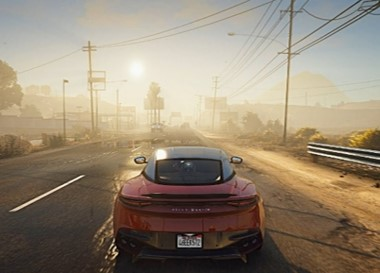
\includegraphics[width=0.45\linewidth]{figures/绪论/1.jpg}
      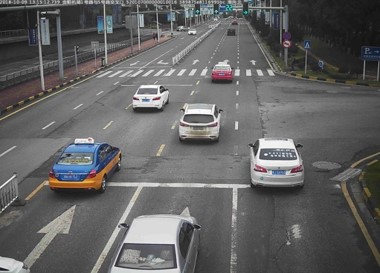
\includegraphics[width=0.45\linewidth]{figures/绪论/2.jpg}
    }
    \subcaptionbox{跨仪器设备医疗影像识别}{
      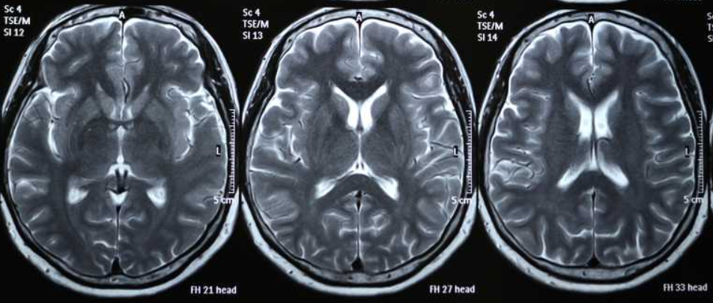
\includegraphics[width=0.52\linewidth]{figures/绪论/ct.png}
      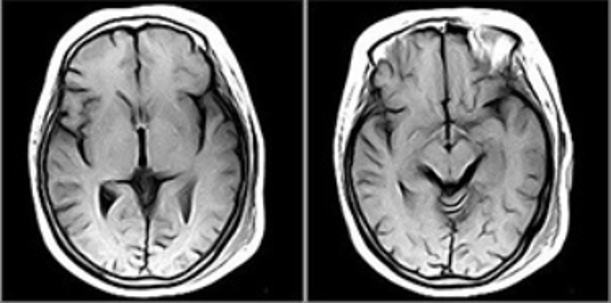
\includegraphics[width=0.46\linewidth]{figures/绪论/核磁.png}
    }
    \caption{迁移学习场景示例}
    \label{fig:transfer}
\end{figure}
    

\subsection{模型微调}

模型微调(Model Fine-tune)是迁移学习中非常重要的子分支之一。这里先对模型微调进行形式化的定义:

\begin{definition}[模型微调]
    假设有一个在源域数据上训练得到的与训练模型$\symup{\Theta}$,以及有$n$条样本的目标域数据集$\mathcal{D}={\{(x_i,y_i)\}_{i=1}^m}$。模型微调的目标是是模型$\symup{\Theta}$在数据集$\mathcal{D}$
    的泛化误差(Generalization Error):
    \begin{equation}
        \mathbb{E}_{(x,y)\sim P_t}[\texttt{Loss}(\symup{\Theta}(x),y)]
    \end{equation}
    最小。
\end{definition}

\begin{figure}
    \centering
    \subcaptionbox{预训练任务}{
        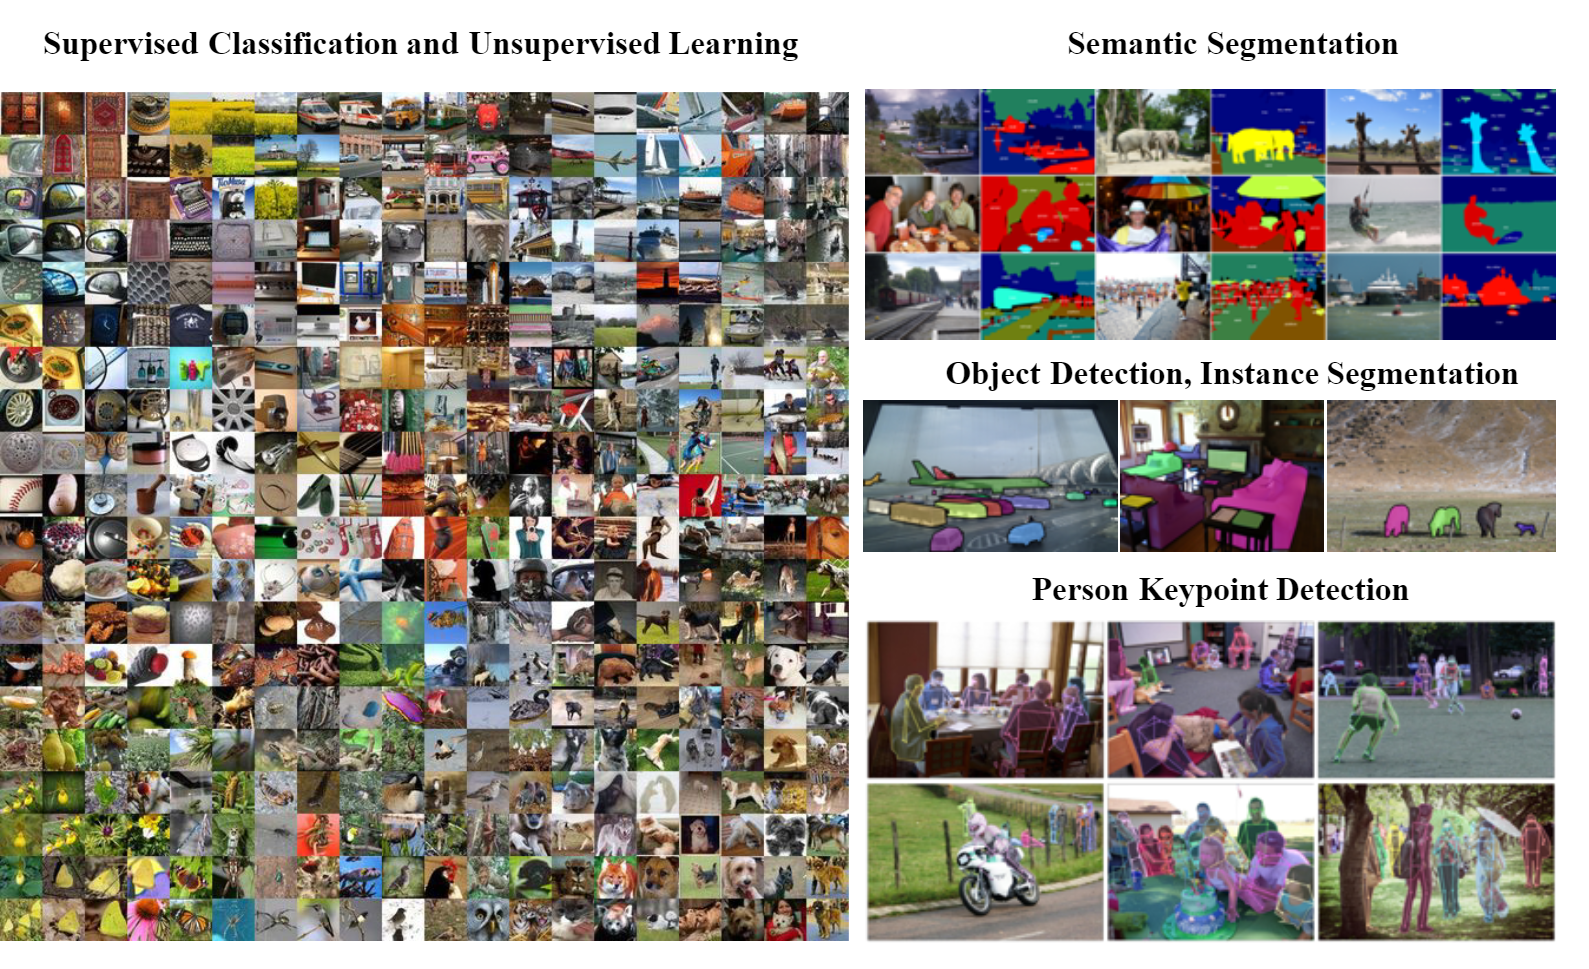
\includegraphics[width=0.9\linewidth]{figures/绪论/pretrain.png}
    }
    \subcaptionbox{模型微调下游任务}{
        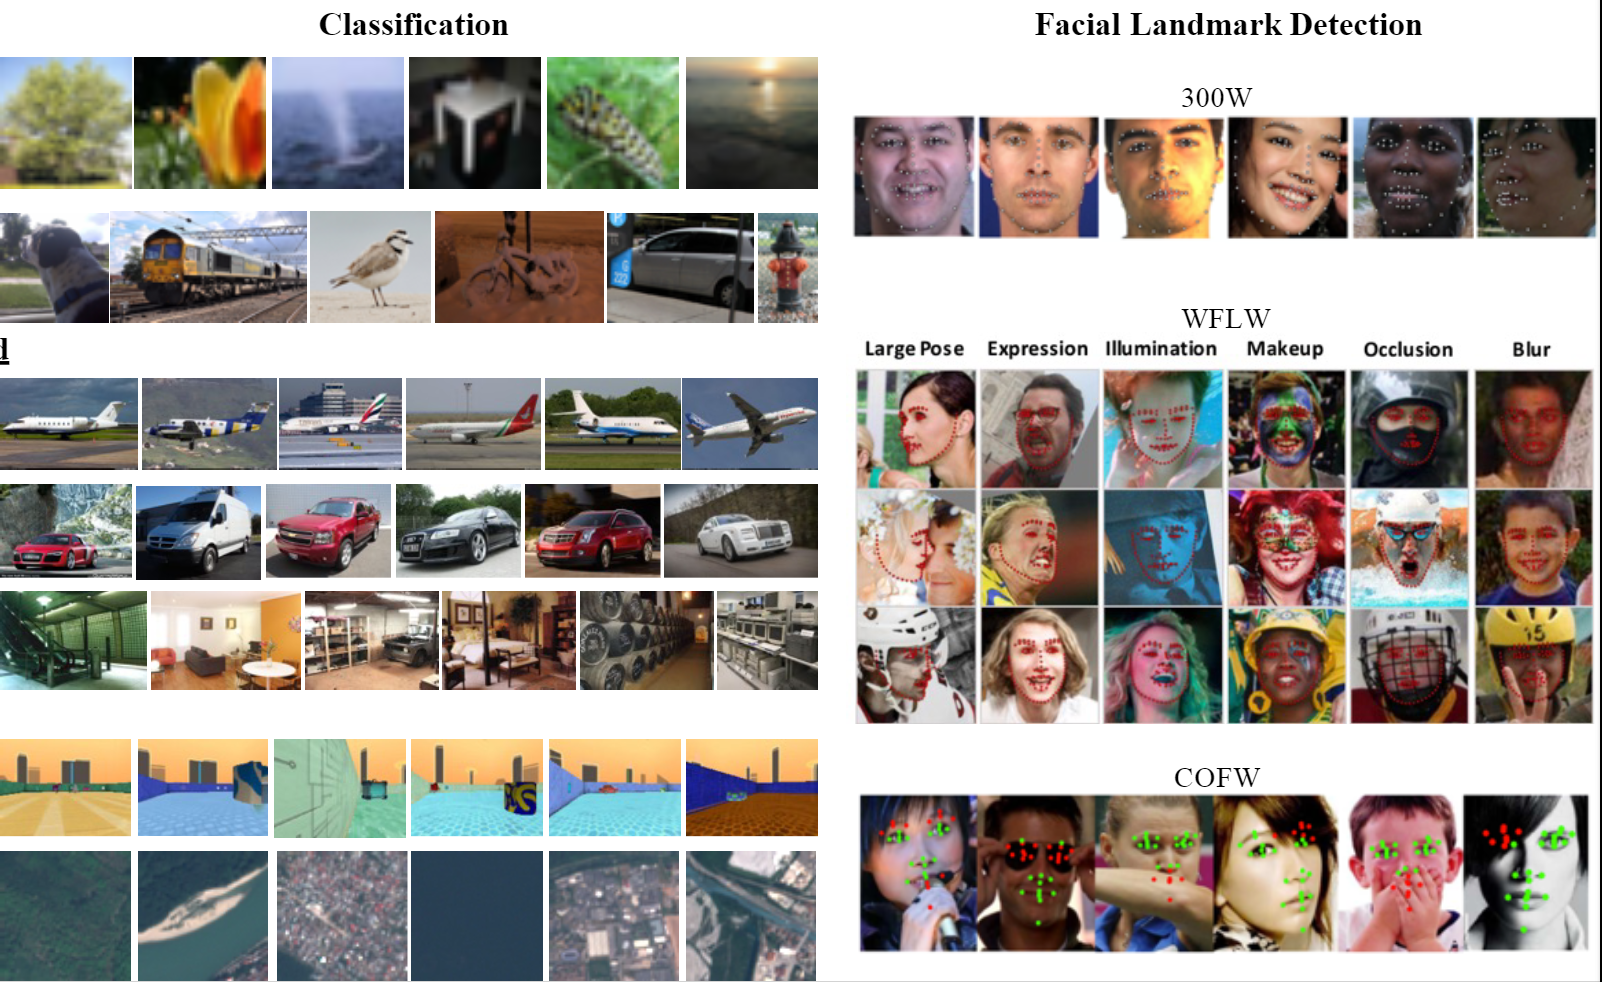
\includegraphics[width=0.9\linewidth]{figures/绪论/finetune.png}
    }
    \caption{一些常见的预训练和微调任务}
    \label{fig:finetune}
\end{figure}

由于在模型微调场景下中,深度神经网络一般无法直接获取源域的训练数据,只能利用在这些数据上训练得到的预训练模型,但相应地在模型微调时可以使用到更大规模的训练数据来提升预训练模型的性能,同时也不会额外
增加训练成本。计算机视觉作为深度学习最先获得成功的领域,一定程度上就是因为天然存在大量的图像作为训练数据,但由于研究人员设计的网络结构日渐复杂,在提升深度神经网络效果的同时,也让深度神经网络逐渐变宽变深,
参数量呈指数式暴涨,使得从头训练一个深度神经网络开始变得极其困难。如果依然在大规模的数据上从头开始进行训练,会消耗大量的时间和计算资源,在这一前提下,模型微调成为了具有很重要的实际意义的研究方向。

模型微调的一大特点便是预训练源域数据集和下游目标域数据集的区别。在很多迁移学习场景中,例如领域适应学习和持续学习,源域和目标域数据一般具有相同的规模、相同的内容或者相同的标签,而模型微调则对两者没有
要求。以图像分类的模型微调场景为例,源域数据集一般包含上万张图像数据,涵盖成百上千种大类,具有很强的通用性和泛化性,但是相应地,预训练阶段所需的时间长、资源消耗巨大;而目标域数据集一般规模较小,具有很强的
目的性,一般是针对某种任务进行数据采集,相应地,微调阶段所需的时间短、资源消耗也明显少于预训练阶段。图~\ref{fig:finetune}展示了一些常见的预训练和微调数据集,可以看出预训练数据数目庞大且具有很强的多样性,
而微调数据集则五花八门,差异明显。模型微调这种方式与人类的学习行为也十分类似,人类在面对新事物时并不会直接参考以往全部的相关事物,而是会直接借助以往积累的经验,即“预训练的知识”快速地做出判断。

在很多实际场景下,数据的采集具有很高的代价和风险,基于目标任务采集的数据可能无法保证深度神经网络得到充分地训练,也就无法充分利用深度学习对数据的学习能力。而模型微调则依靠
具有很强通用性和泛化性的预训练模型,在高效利用预训练知识的同时,也很大程度上弥补了下游任务中数据量不足的缺陷,为深度学习的广泛应用创造了无限可能。

\section{研究问题与挑战}

深度学习的发展离不开深度神经网络结构的进步,而无论什么类型的深度神经网络,都离不开标准化层结构。尽管标准化层的设计和算法实现通常比较简单,但是在什么维度进行标准化、如何标准化、为什么要进行标准化等问题,
关系着最终网络性能能否提升。研究人员针对各种任务场景,设计了特有的标准化层结构,从结构层面提高了深度神经网络的性能,取得了非常显著的成果。但是这些结构往往依据该场景下的一些先验假设,
在其他场景中可能不会有效,甚至带来负效应。

利用预训练模型进行模型微调,作为深度学习中使用非常广泛的方法,在许多实际应用场景下都取得了很好的效果。然而目前针对模型微调场景的标准化层结构研究还较为欠缺,研究人员往往选择继承预训练模型使用
的标准化层而不作任何修改。尽管大部分情况下这种方式不会带了负面影响,但是依然忽视了很多模型微调中特有的问题,存在着很大的改进空间。因此,本文选择模型微调场
景下的标准化层为研究课题,旨在分析模型微调场景下现有标准化方法的不足,并针对性地设计全新的标准化层结构,提升模型微调算法的效果。

\section{研究现状}

本节对模型微调以及标准化层领域的相关工作进行简要地概括,在下一章中会进行更加详细的介绍。

\subsection{模型微调}

模型微调领域下根据研究阶段的不同分为预训练阶段和微调阶段。预训练阶段的主要研究问题为如何设计具有更好通用性和泛化性的预训练模型,包括但不限于更大的预训练数据集、更复杂的深度神经网络、更强的预训练技术等等。
一部分数据科学家们会耗时数年构建一个非常庞大的预训练数据集~\citep{deng2009imagenet,sun2017revisiting},而一部分研究工作则针对设计更宽更深的深度神经网络结构~\citep{szegedy_going_2015,szegedy2016rethinking,
he2016deep,huang_densely_2017}。另外一些工作则在前两者的基础上,通过设计新的预训练方式来获得更强的预训练模型,使用诸如掩码模型(Masked Modeling)~\citep{devlin2019bert,bao2021beit,he2021masked}、
对比学习(Contrastive Learning)~\citep{he2020momentum,chen_simple_2020}、提示学习(Prompt Learning)~\citep{liu2021pre,radford2021learning}等方法,进一步挖掘预训练模型的潜力。

而在微调阶段,则更关注于如何基于下游任务的特性,最大程度地利用预训练模型中的知识。在微调阶段,最为常见的研究问题便是灾难性遗忘(Catastrophic Forgetting),会使得深度神经网络在学习下游任务知识的
同时,逐渐丢失预训练模型中的知识,这与模型微调的初衷相悖。因此有很大一部分研究工作针对这一问题,使用基于正则化约束的方法来避免对预训练模型知识的遗忘~\citep{li2017learning,li2018delta,li2018learning,you2020co}。
而有些工作则着眼于不同预训练模型对微调任务的影响,Kornblith等人的工作~\citep{kornblith2018better}通过使用不同深度神经网络结构的预训练模型在不同的下游任务上进行微调,得出了一系列预训练模型对微调影响的结论。
基于这一发现,一些工作提出了对不同的预训练模型进行评判的准则,先选出最适合当前下游任务的预训练模型再进行微调~\citep{tran2019transferability,bao2019information,you2021logme}。也有一些研究人员认为,并不需要
对预训练模型进行筛选,直接对多个预训练模型的特征或者参数进行集成能更大程度上利用预训练的知识~\citep{rusu2016progressive,liu2019knowledge,shu2021zoo}。


\subsection{标准化层}

如今深度学习的迅速发展离不开深度神经网络结构的改进,从最早的多层感知机(Multi-Layer Perceptron,MLP)到卷积神经网络(Convolutional Neural Networks,CNN)和循环神经
网络(Recurrent Neural Networks,RNN),再到目前最为引人注意的Transformer,深度神经网络的每一次迭代,都在各类深度学习任务上取得了标志性的提升。
但是纵观这些风格各异的深度神经网络,在网络规模变大的同时,都离不开一个重要的组件——标准化层。例如多层感知机和卷积神经网络中的批标准化(Batch Normalization)~\citep{ioffe2015BN},循环神经
网络和Transformer中的层标准化(Layer Normalization)\citep{lei2016LayerNorm}等等。

标准化最早是统计学中的概念,一般指参照某一个统一的标准来调整两组数据的构成,从而使其能够互相比较。最常见的标准化便是对一组数据${\{x_i\}}_{i=1}^n$,先计算它们的
均值和方差:
\begin{equation}
\begin{aligned}
    \mu=\frac{1}{n}\sum_{i=1}^n{x_i},\quad
    \sigma^2=\frac{1}{n}\sum_{i=1}^{n}{(x_i-\mu)^2}
\end{aligned}
\end{equation}

再将整组数据减去均值除以方差:

\begin{equation}
    x'=\frac{x-\mu}{\sigma}
\end{equation}

从而使得这组数据的均值为$0$而方差为$1$。

深度学习中对标准化的利用非常丰富,实际场景下主要根据任务的不同,可以在不同的维度上计算特征的均值$\mu$和方差$\sigma$~\citep{ioffe2015BN,lei2016LayerNorm,ulyanov_instance_2016,wu2018GroupNorm},
或者对特征之外的数据,诸如网络参数或者特征的奇异值等进行标准化~\citep{Salimans2016Weight,miyato_spectral_2018}。正是由于标准化技术的多样性,不同的标准化层在不同任务中的效果往往差别很大,
研究人员需要根据实际场景选择或者设计更合适的标准化层结构。

\section{研究内容与主要创新点}

图~\ref{fig:research}为本文的研究框架图。本文主要通过研究深度神经网络结果,设计了一种全新的标准化层,从而提升网络的整体性能,接着在学术界使用的细粒度分类任务上进行了实验,并在实际场
景中的医疗影像任务和风速预测任务进一步验证了其效果,最后借助迁移学习算法库的平台对该标准化层结构进行了集成。

\begin{figure}
    \centering
    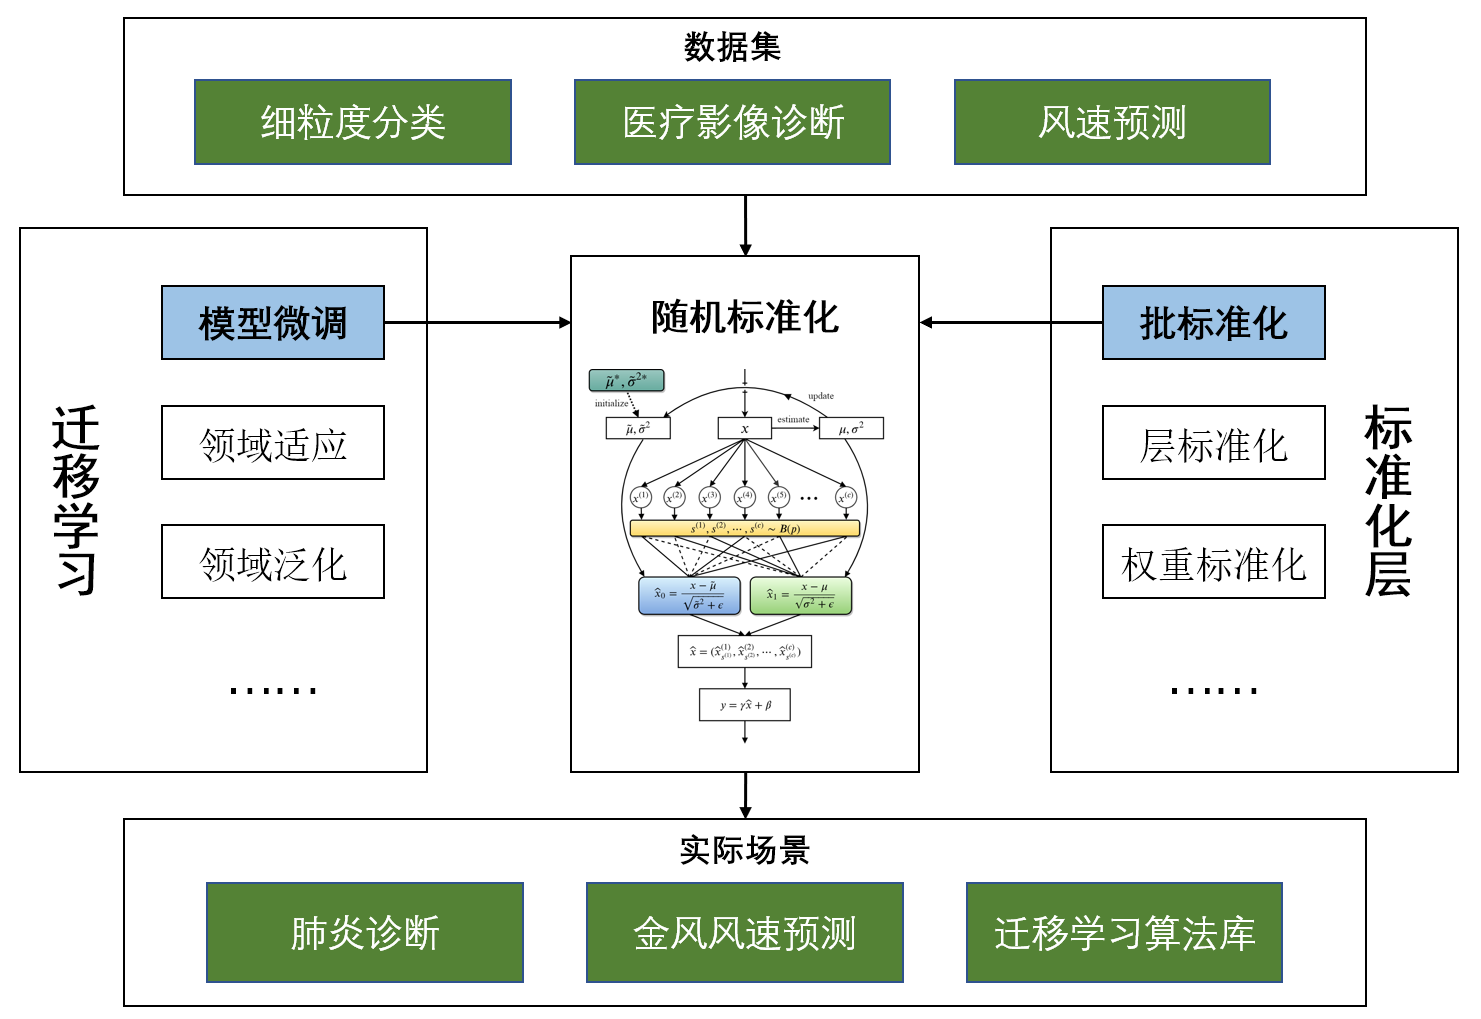
\includegraphics[width=\linewidth]{figures/绪论/arch.png}
    \caption{研究框架图}
    \label{fig:research}
\end{figure}

本文的主要创新点以及贡献如下:
\begin{itemize}
    \item 本文设计了一种全新的标准化层——随机标准化层(Stochastic Normalization,StochNorm),该标准化层超参数较少且结构简洁,具有很好的通用性,能够高效快捷地和现有的深度神经网络结构以及模型微调方法相结合。
    \item 本文针对模型微调场景,在多个细粒度图像分类数据集上使用带有StochNorm的深度神经网络进行训练,相较于传统的模型微调方法取得了明显的提升,并且能够很好地和这些方法进行结合,进一步提升效果。该部分算法研究成果发表在了机器学习顶级会议\textbf{NeurIPS-2019}(CCF-A,清华A类)上。
    \item 本文针对医疗影像诊断和金风风速预测两个实际场景,在基线深度神经网络结构中加入了StochNorm技术,均取得了一定的效果提升;
    \item 本文借助迁移学习算法库(Transfer Learning Library)的平台对StochNorm算法进行了集成与复现,取得了与本文实验部分一致的提升效果,提供了快捷调用的API接口。
\end{itemize}

\section{文章结构安排}
本文共计5个章节,主要内容安排如下:

第1章为绪论,主要介绍了本文的选题背景与意义,介绍了主要针对的两个场景,概括了本文的创新点和主要贡献。

第2章为相关工作介绍,介绍了模型微调领域和标准化层领域的发展历程和最新工作。

第3章主要介绍了本文提出的随机标准化层的算法细节,并在多个细粒度分类数据集上设计了实验,验证了该算法的性能。

第4章展示了StochNorm在实际场景中的应用,在医疗影像诊断和金风风速预测两个场景验证了该算法的有效性,并在迁移学习算法库中进行了集成,提供了快捷调用的API。

第5章对本文的工作进行了总结,并对未来工作进行了展望。

% !TeX root = ../thuthesis-example.tex

\chapter{相关工作}

\section{模型微调研究现状}

\subsection{预训练技术}

作为迁移学习中最为经典的方法之一,模型微调(Model Fine-tune)的成功离不开离不开模型预训练技术的发展。在深度学习诞生初期,训练数据较少而深度神经网络结构也比较简单,
研究人员往往直接使用基于随机初始值初始化的网络在训练数据上从头开始训练。但是随着数据科学和算力资源的快速发展,这种方式往往需要极其庞大的计算集群连续训练很久很久,对于
普通科研人员以及许多实际场景而言并不现实。Donahue和Oquab~\citep{donahue2014decaf,oquab2014learning}等人的工作发现,训练好的AlexNet提取到的图像特征,可以被迁移到
很多不同的任务中,而且效果明显好于人工设计的特征。这一发现启发了学术界,很多工作~\citep{agrawal2014analyzing,girshick2014rich}也进一步证实,基于预训练的网络参数
进行微调相比完全使用固定的特征提取器能够取得更好的效果。甚至在目标域数据集和预训练数据集完全不同这种更为极端的情况下,模型微调即使无法带来明显的提升~\citep{raghu2019transfusion},
也依然能够加速模型的收敛~\citep{he2018rethinking}。

计算机视觉中卷积神经网络的演变也代表了预训练技术早起的发展,而作为计算机视觉中最为知名的任务,ImageNet-1K~\citep{deng_imagenet:_2009}也成为了预训练技术中最为广泛使用的数据集。
从最早的在ILSVRC2012图像识别竞赛中大放异彩的AlexNet,到通过巧妙设计不断加深网络层数的VGG~\citep{szegedy_going_2015}和引入不同大小卷积核并行结构的Inception Net~\citep{szegedy2016rethinking},
再到使用跳层链接(Skip Connections)实现超深网络结构的ResNet~\citep{he2016deep}和利用密集连接进一步提升效果的DenseNet~\citep{huang_densely_2017},不同结构的深度神经网络在
一次次刷新ImageNet图像分类任务新纪录的同时,也为学术界带来了一个又一个预训练模型。这些基于ImageNet的预训练模型在图像分类、目标检测(Object Detection)、图像识别(Image Recognization)、
语义分割(Semantic Segmentation)等领域都获得了极大的成功。

尽管一直以来的经验认为,网络的深度对模型的性能至关重要,但是深度残差网络(Deep residual network, ResNet)中作者发现,随着深度神经网络深度的增加,
网络的准确度反而达到瓶颈甚至下降,出现了所谓网络退化的现象。作者认为,网络深度的增加会使得网络的容量(Capacity)增大,使其更不容易学习。为了解决退化问题,作者引入了残差机制,对于某个
输入$x$以及其经过网络层后得到的输出$H(x)$,残差学习的目标是学习$F(x)=H(x)-x$这一残差项,那么原始要学习的特征便是$F(x)+x$。当残差为$0$时,网络层的行为就是恒等映射,至少不会使网络的性能下降;
而残差不为$0$时,便意味着网络层在输入$x$的基础上学习到了新的特征。残差结构~\ref{fig:residual}如图所示。ResNet通过引入残差学习的机制,成功将网络深度大幅拓展,也在各类计算机视觉任务中刷新了最好效果。

% 图~\ref{fig:densenet}为DenseNet的示意图。

\begin{figure}
    \centering
    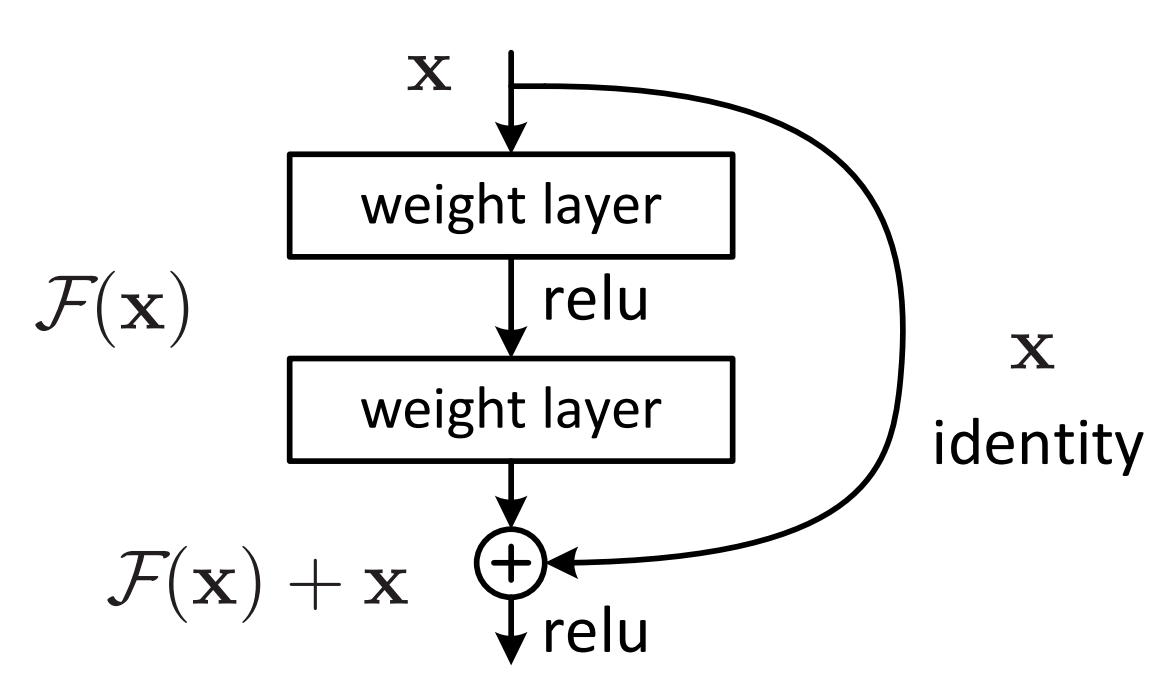
\includegraphics[width=0.5\linewidth]{figures/residual.png}
    \caption{残差结构~\citep{he2016deep}}
    \label{fig:residual}
\end{figure}

深度神经网络的训练技术在自然语言处理(Natural Language Processing,NLP)领域也取得了非常有意义的成果。Word2Vec~\citep{mikolov2013distributed}和Glove~\citep{pennington2014glove}等工作提供了预训练得到的词向量表征,但是在下游任务
中依然需要从头训练更高层级的语义表示。BERT~\citep{devlin2019bert}则通过在掩码语言模型(Masked Language Modeling)上进行预训练,获得了非常强大的预训练表征,使得很大一部分下游任务只需要基于BERT进行微调,就能
取得很好的效果。BERT的结构如图~\ref{fig:bert}所示,它的提出再一次证明了预训练技术的强大与可靠,各种各样基于BERT改进的预训练模型在NLP的各类任务上不断刷新最好成绩。

\begin{figure}
    \centering
    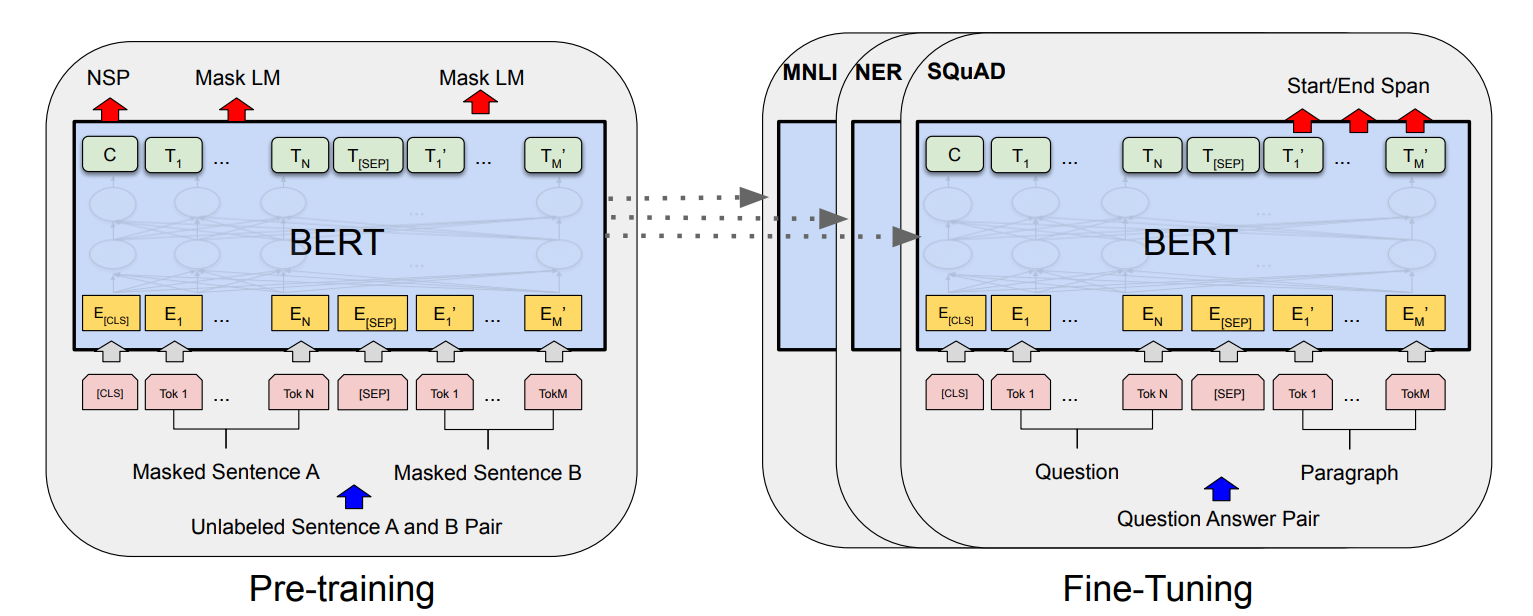
\includegraphics[width=\linewidth]{figures/bert.png}
    \caption{Bert结构~\citep{devlin2019bert}}
    \label{fig:bert}
\end{figure}

图~\ref{fig:bert}为Bert的结构示意图。传统的自然语言处理领域的预训练模型,会受到单向语言模型的限制,只能在一个方向上获得上下文的信息。Bert(Bidirectional Encoder Representation from Transformers)
则顾名思义,是一个双向预训练得到的语言表征(representation)模型。Bert的一种预训练方式是基于掩码语言模型进行的,在预训练序列中以一定概率随机将字符(token)替换为掩码[MASK],再使用模型去预测这些掩码位置对应的字符,
这种方式使得模型不再受单向语言模型的限制,同时对所有的字符都敏感,从而抽取出足够强大的语言表征。Bert可以说是自然语言处理领域最为成功的预训练模型之一,通过基于Bert进行模型微调,在许多自然语言处理任务上取得了当时最好的效果。

传统的基于单一类型数据训练得到的模型,往往会局限于定义好的数据类别中进行预测,一旦遇到从未见过的数据,效果会显著下降。为了解决这一问题,研究人员将目光转向了多模态的预训练模型,希望通过拓展预训练的维度来获得更泛化的预训练模型。
在多模态预训练模型CLIP~\citep{radford2021learning}中,深度神经网络的输入不再是单一的图像数据,而是额外加入了自然语言对图像的描述作为提示信息(prompt),使用这种带有描述的图像进行训练得到的模型具有更好的泛化性,
在小样本学习(Few-shot Learning)、零样本学习(Zero-shot Learning)中有着更好的表现。
图~\ref{fig:clip}为CLIP的结构示意图。

\begin{figure}
    \centering
    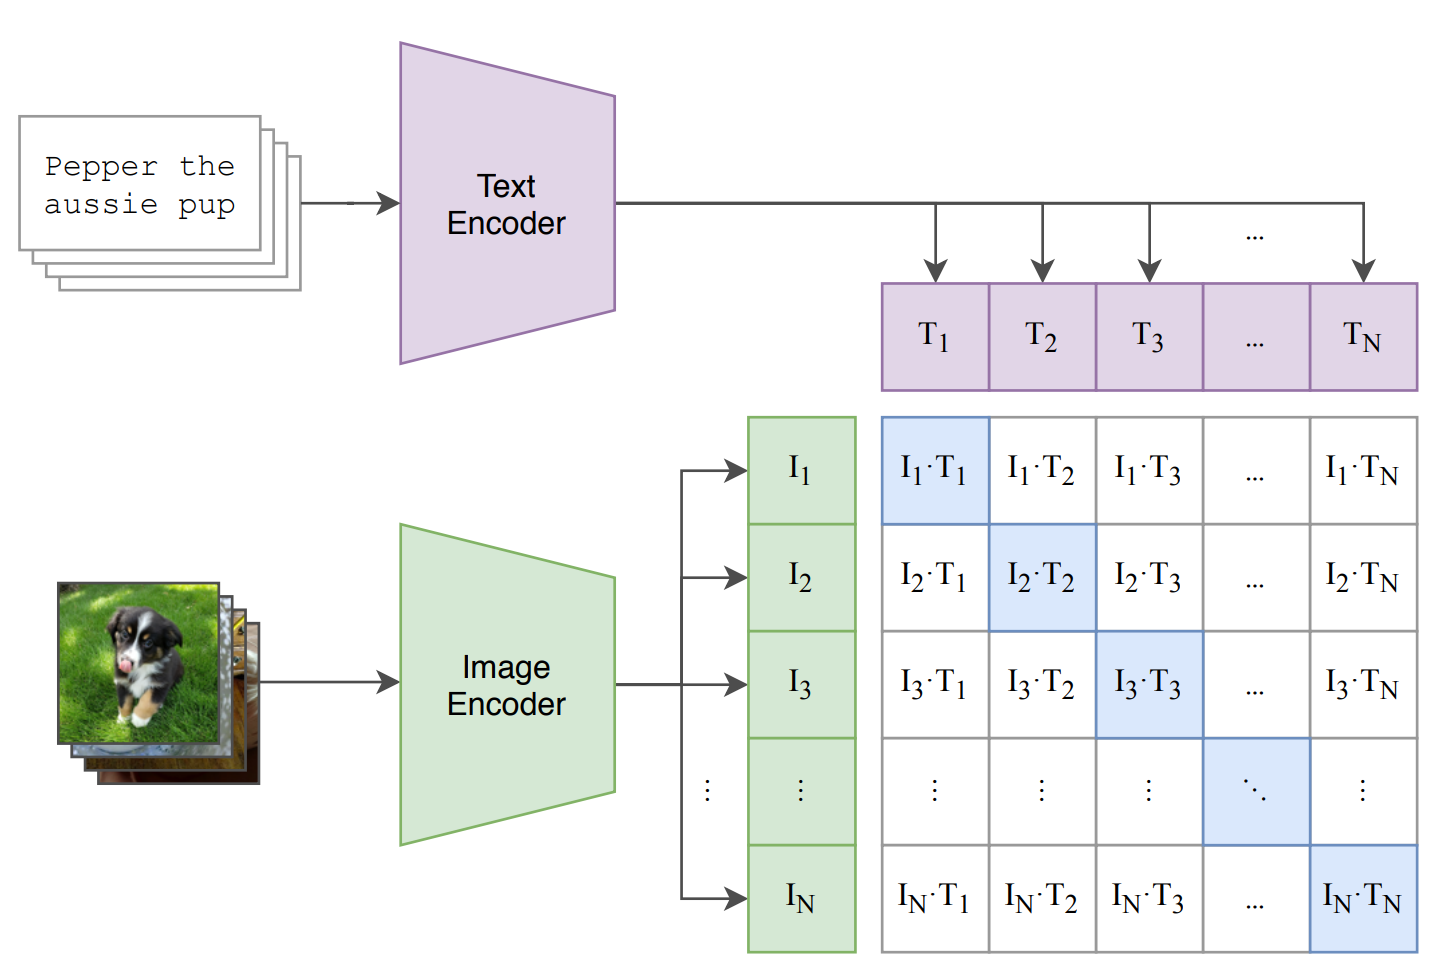
\includegraphics[width=0.8\linewidth]{figures/clip.png}
    \caption{CLIP的结构图~\citep{radford2021learning}}
    \label{fig:clip}
\end{figure}

\subsection{灾难性遗忘与负迁移}

尽管预训练技术的发展为研究人员提供了多种多样预训练模型的选择,但是在模型微调阶段依然会遇到各种各样的困难,其中灾难性遗忘(Catastrophic Forgetting)与负迁移(Negative Transfer)是很常见的两个问题。

依照顺序方式学习任务的能力对于人工智能的发展是至关重要的,然而一直以来对于深度神经网络,灾难性遗忘都是很难避免的。灾难性遗忘是指在新的任务上进行训练时,深度神经网络会逐渐丢失旧任务的相关信息,导致无法
按照预期进行顺序学习,这与网络的连接式结构、网络优化的方式等因素都有关系~\citep{french1999catastrophic}。
模型微调就是一种非常经典的顺序学习范式,在使用目标域数据对预训练模型进行微调时,由于带有标注的训练数据往往非常稀少,导致模型容易逐渐忘记预训练模型中的知识,产生过拟合,
也被称为表征崩坏(representational collapse),体现为原本依靠预训练技术得到表征的泛化性随着训练的进行逐渐减弱~\citep{aghajanyan2020intrinsic}。
研究人员一直以来都在为解决这一问题进行不断的尝试,最简单的方法便是选择较小的学习率并且使用提前停止(early-stopping)的技术,从而避免模型参数更新程度过大。但是这种方法很容易
使得模型陷入局部最优值,尤其是当下游任务差异较大时愈加明显。

\begin{figure}
    \centering
    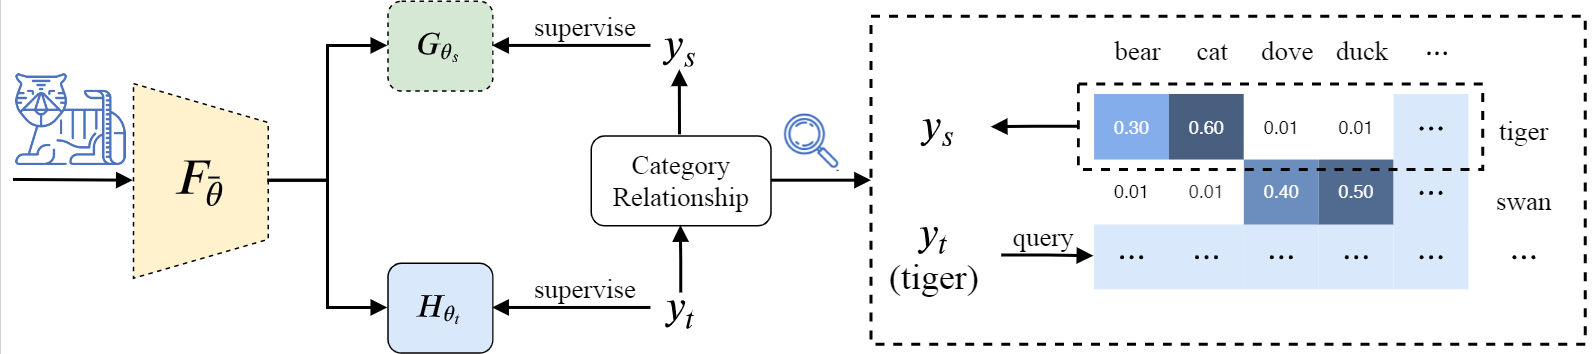
\includegraphics[width=\linewidth]{figures/cotuning.png}
    \caption{Co-Tuning的示意图~\citep{you2020co}}
    \label{fig:cotuning}
\end{figure}

基于正则化约束的模型微调时解决灾难性遗忘的一种经典且有效的方法。
最直接的方式便是直接通过约束网络的预测结果来控制网络的训练,Learning Without Forgetting~\citep{li2017learning}便是其中的代表工作。LWF中认为,在不同域的数据集之间可以共享一个通
用的特征提取器,只需要分别使用各自对应的分类器即可获得很好的效果。由于灾难性遗忘的一大表现是在新任务上获得提升的同时在过去任务上显著下降,因此LWF在新任务上使用新的分类器进行微调的同时,依然保持对所有旧任务分类器的训练。
这种训练范式自然而然地能在保证新任务模型效果的同时不遗忘过去任务中的知识。这种思路也被拓展到了图像分类以外的任务上,取得了不错的效果。
Co-Tuning~\citep{you2020co}则直接利用预训练模型分类器中的知识,建模了源域数据标签空间和目标域标签空间间的映射关系,并利用这一映射关系在模型微调阶段生成伪标签辅助训练,
从另一种角度对网络的预测结果进行了约束,一定程度上避免了灾难性遗忘。Co-Tuning的结构如图~\ref{fig:cotuning}所示。

另一种方式则是通过间接约束网络的参数、特征图等信息,来控制网络的训练。直观上来讲,具有相似参数的网络(层)产生的输出也应该相似,基于这一思想,$L_2$-SP~\citep{xuhong2018explicit}中直接约束特征提取
器的网络参数,避免在模型微调阶段中与预训练模型参数之间差异过大,从而间接约束了网络的输出。而DELTA~\citep{li2018delta}中则选择约束网络中间层输出的特征图,通过注意力机制对特征进行重要性加权,选出
更具有迁移性和判别性的特征。其结构如图~\ref{fig:delta}所示。

\begin{figure}
    \centering
    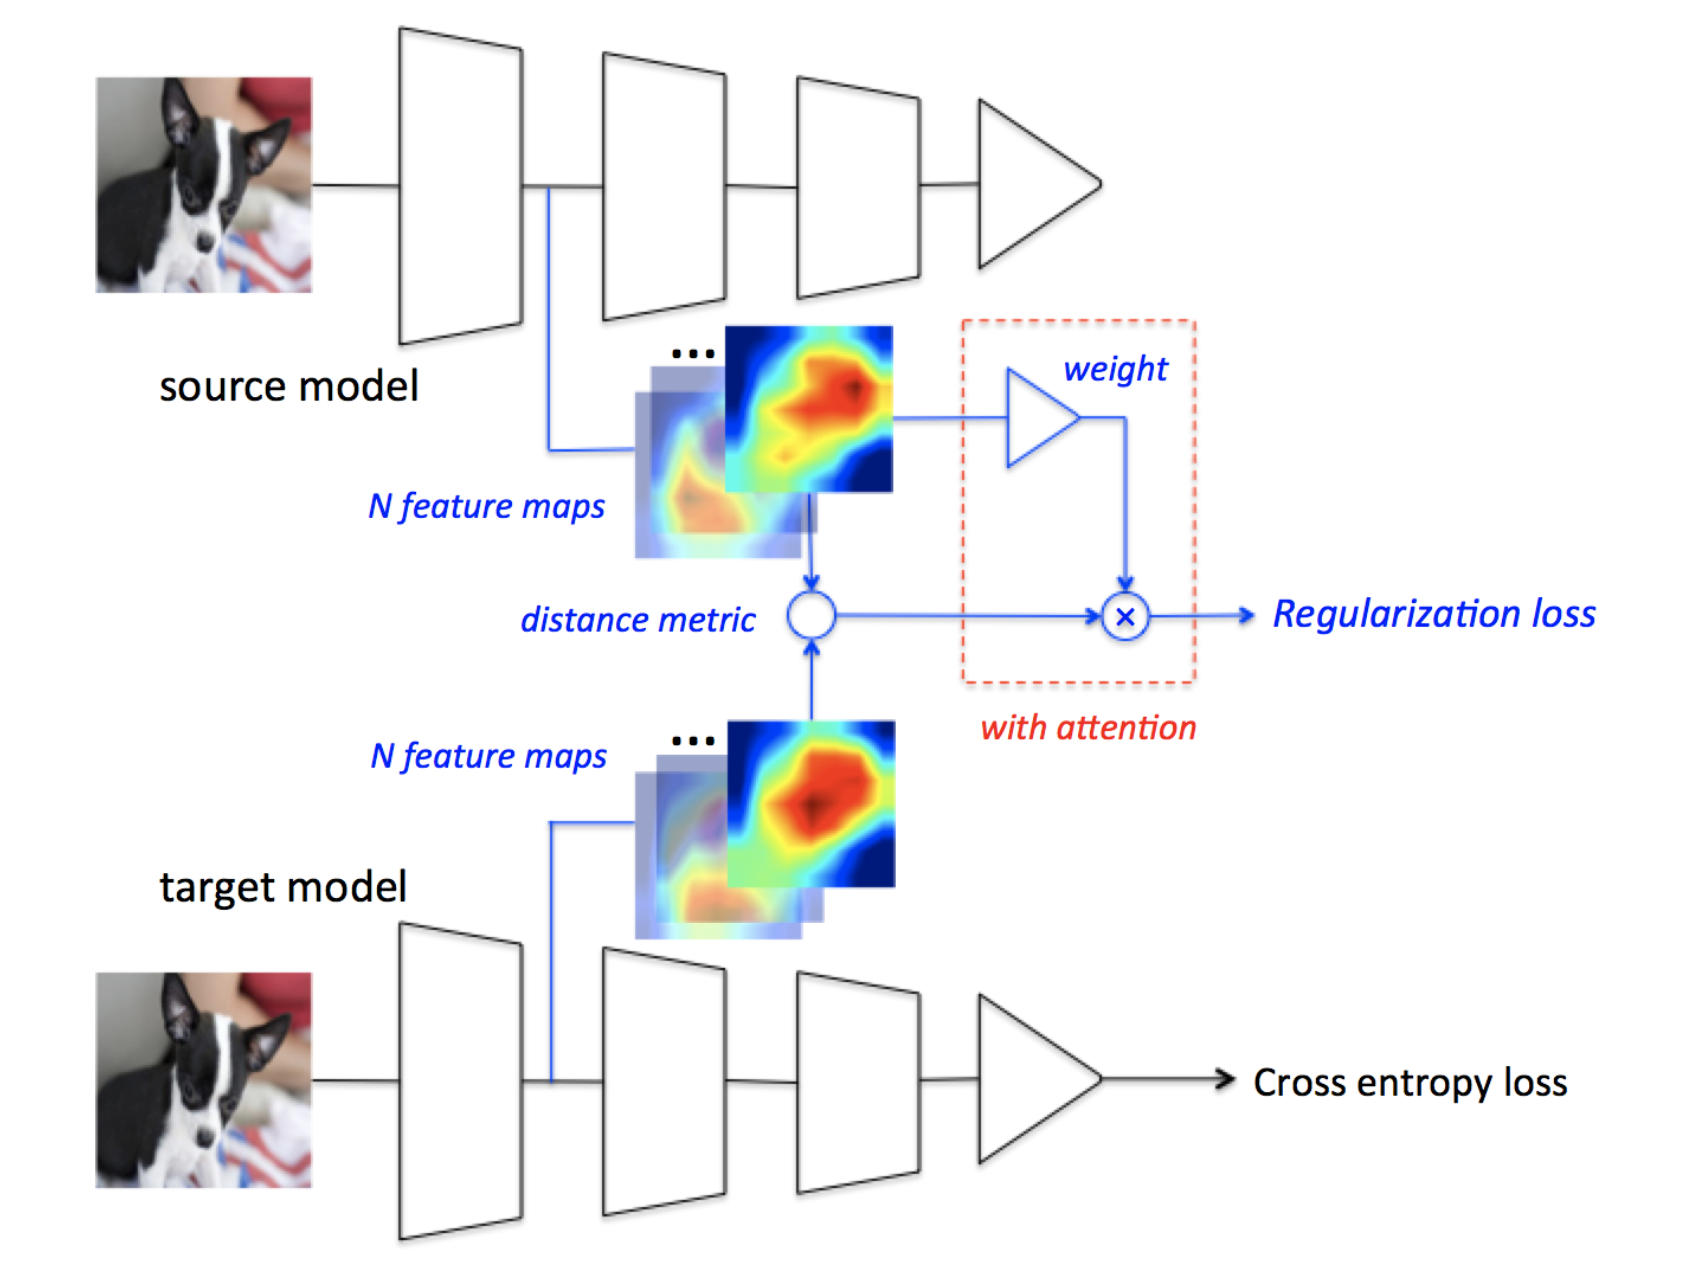
\includegraphics[width=0.8\linewidth]{figures/delta.png}
    \caption{DELTA的示意图~\citep{li2018delta}}
    \label{fig:delta}
\end{figure}

在很长一段时间内,灾难性遗忘都是模型微调领域中非常热门的问题。但是随着研究的深入,研究人员发现在目标域和源域数据差异过大的情况下,过度约束网络的输出、参数以及特征图反而会带来负收益。在BSS~\citep{chen2019catastrophic}中,
作者认为这一现象是因为发生了负迁移。负迁移是指在迁移学习中,由于过度重视预训练模型中的知识而忽略了目标域数据上的特性,迁移了许多不具备迁移性,或者在目标数数据上并不合适的知识,从而影响模型最终效果的现象。

\begin{definition}[负迁移~\citep{wang2018characterizing}]
    令$A(P_s,P_t)$为算法$A$在数据分布$P_s$上预训练得到的模型在数据分布$P_t$上微调得到的模型,$A(\emptyset,P_t)$为在算法$A$在数据分布$P_t$上直接从头训练得到的模型,称
    \begin{equation}
        \mathbb{E}_{(x,y)\sim P_t}[\texttt{Loss}(A(P_s,P_t)(x),y)] > \mathop {\min} \limits_{ A'} \mathbb{E}_{(x,y)\sim P_t}[\texttt{Loss}(A'(\emptyset,P_t)(x),y)]
    \end{equation}
    为负迁移。
\end{definition} 

负迁移在人类的学习任务中也很常见,许多基于经验的知识在面对完全陌生的问题时,往往会让人陷入思维定势。BSS~\citep{chen2019catastrophic}中作者分析了负迁移发生的情况以及原因,并基于谱分析(Spectral Analysis)的技术设计了基于特征图
奇异值分解后得到的奇异值的损失函数,一定程度上避免了负迁移现象的发生。

除了使用约束项避免负迁移外,合理地挑选预训练模型也是解决负迁移的方法之一。早期的研究工作认为任何预训练模型对于下游任务来说都是有益的,但是负迁移现象意味着,当预训练数据与下游任务数据差别过大时,使用这样的
预训练模型会带来负收益。Taskonomy~\citep{zamir_taskonomy:_2018}提出了一种基于任务相关性进行快速挑选的算法;LEEP~\citep{nguyen2020leep}则对预训练数据和下游任务数据标签的联合分布进行预测,利用预测值来衡量预训练
模型的迁移性。但是He等人的工作~\citep{he2021masked}通过实验证明,通过对比式预训练(Contrastive Pre-training)得到的特征在模型微调中的效果并不如生成式预训练(Generative Pre-training),尽管前者具有更好的线性分类
准确率,这意味着预训练模型特征的线性可分性并非评判其迁移性的可靠指标。

\subsection{多模型迁移}

目前学术界的大多数模型微调工作都基于单个预训练模型进行,预训练模型的发展局限于深度神经网络结构的更新。然而随着数据科学的发展,越来越多的预训练数据集被提出,诸如包含了远超ImageNet-1K数据集几个数量级
的ImageNet-21K~\citep{deng2009imagenet}以及JFT-300M~\citep{sun2017revisiting}数据集。预训练任务也不再局限于有监督的图像分类,MoCo~\citep{he2020momentum}和SimCLR~\citep{chen_simple_2020}
尝试利用无监督的训练数据进行预训练,获得了接近于有监督预训练的效果,极大程度上降低了预训练数据的采集难度;He等人的工作~\citep{he2017mask}也提供了在目标检测与实例分割任务上预训练得到的Mask R-CNN模型;
Chen等人的工作~\citep{chen2018encoder}则提供了在语义分割上预训练得到的DeepLab模型。

\begin{figure}
    \centering
    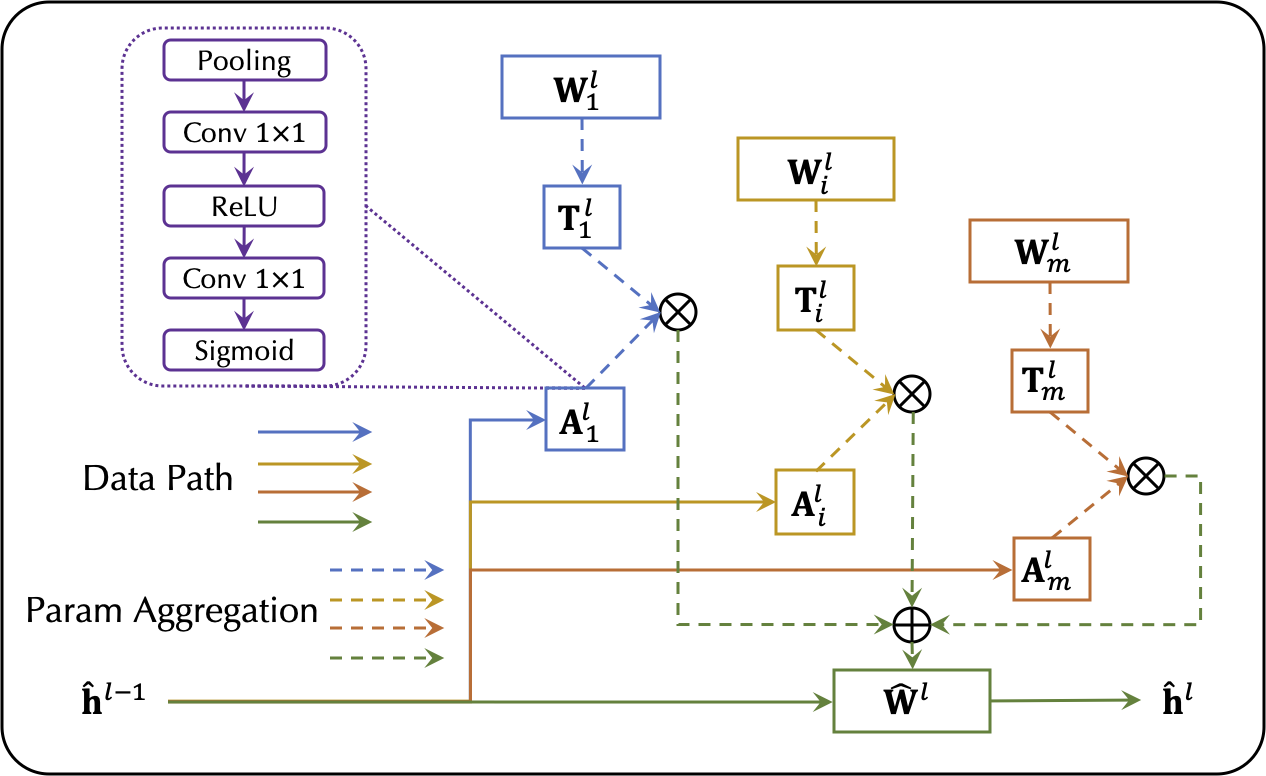
\includegraphics[width=0.8\linewidth]{figures/zootuning.png}
    \caption{Zoo-Tuning的示意图~\citep{shu2021zoo}}
    \label{fig:zoo}
\end{figure}

面对数目众多且任务各不相同的预训练模型,一些工作尝试通过某种机制从预训练模型中选出最适合下游任务的一个进行模型微调~\citep{tran2019transferability,bao2019information,you2021logme},这种方法虽然
将多模型迁移(Multi-model Transfer)与传统的模型微调方法结合了起来,但是仍然有一些不足之处:对预训练模型的筛选机制往往基于某些先验假设,可能并不准确;其次只有一个预训练模型最终被使用,没能充分利用到
如此多预训练模型中的丰富知识。这部分工作还局限于传统模型微调的架构,但是也为之后多预训练模型迁移的研究做出了贡献。一些工作则尝试将不同预训练模型提取的特征进行组合,从而利用预训练模型的先验知
识~\citep{rusu2016progressive,liu2019knowledge},但是这些方法往往需要同时保存多个预训练模型的网络参数,并且要同时提取多种特征,造成了很高的计算和内存消耗。其次,直接使用预训练模型提取的特征而完全
不做针对目标域数据的适应,也很容易在下游任务较为困难,或者和预训练任务有较大的区别时带来负提升。Shu等人的工作~\citep{shu2021zoo}则直接从预训练模型的网络参数角度出发,引入注意力机制计算不同预训练模型
对目标域数据的重要程度,再根据注意力权重对网络参数进行重新组合,从而在不额外增加计算代价的前提下充分利用多个预训练模型中的知识,其结构如图~\ref{fig:zoo}所示。

\section{标准化层}

\subsection{标准化层研究现状}

Boyd等人的工作~\citep{boyd_convex_2004}发现,对输入进行标准化能够对深度神经网络的训练起到帮助,是因为诸如随机梯度下降(Stochastic Gradient Descent,SGD)的一阶优化算法在目标函数曲面更加平滑时效果更好。随后
Ioffe等人的工作~\citep{ioffe2015BN}则提出了批标准化(Batch Normalization)的算法,对网络的输入根据其均值和方差进行标准化,很大程度下帮助了深度神经网络的训练。受BatchNorm的启发,现在深度学习工作中出现了越来越多
的标准化层技巧。层标准化(Layer Normalization)\citep{lei2016LayerNorm}和循环批标准化(Recurrent Batch Normalization)\citep{cooijmans2016recurrent}在循环神经网络的训练中非常有效;组标准化(Group Normalization)
\citep{wu2018GroupNorm}则是为目标检测任务专门设计的;实例标准化(InstanceNormalization)\citep{ulyanov_instance_2016}则提升了风格迁移(Style Transfer)任务的效果。
图~\ref{fig:norm}中展示了这其中的几种标准化层结构的区别。
\begin{figure}
    \centering
    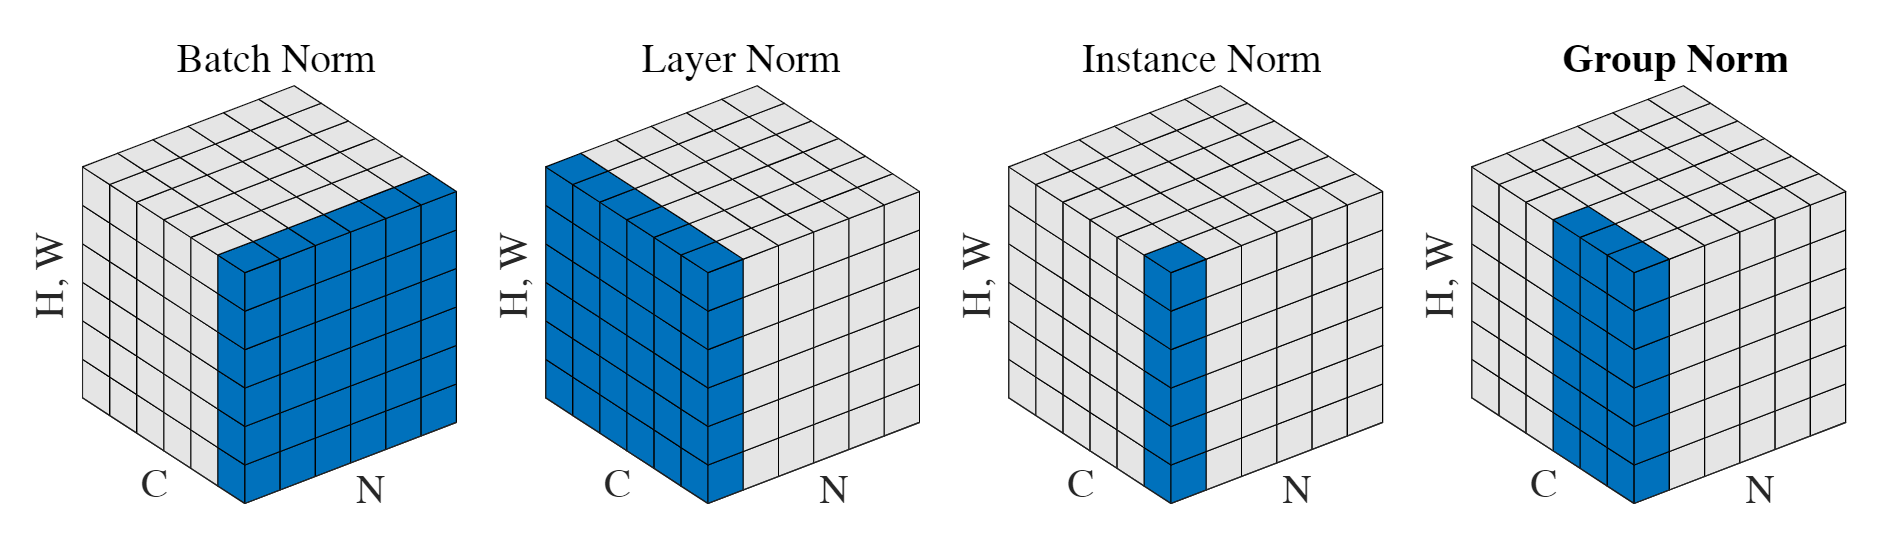
\includegraphics[width=\linewidth]{figures/norm.png}
    \caption{几种标准化层的示意图~\citep{wu2018GroupNorm}}
    \label{fig:norm}
\end{figure}

除此之外,还有一部分标准化层针对深度神经网络的参数进行标准化,例如权重标准化(Weight Normalization)\citep{Salimans2016Weight}则通过简单的重参数化(re-parameterization)
加速了随机梯度下降的收敛速度;谱标准化(Spectral Normalizaiton)\citep{miyato_spectral_2018}则通过约束网络参数的最大特征值从而保证模型满足
1-利普希茨连续(1-Lipschitz continuous),从而避免生成式对抗网络(Generative Adversarial Networks,GAN)中的模型崩溃问题,

\begin{definition}[权重标准化与谱标准化]
    对于深度神经网络中的非线性层以及输入$x$,输出$y$可以表示为:
    \begin{equation}
        y=\phi(\mathbf{w}\cdot \mathbf{x} + b)
    \end{equation}
    其中$\phi$表示激活函数,$\mathbf{w}$为权重向量,$b$为偏移(bias)标量。

    权重标准化中使用与$\mathbf{w}$相同尺寸的向量$\mathbf{v}$和标量$s$对非线性层中的网络参数$\mathbf{w}$进行重参数化,将方向与长度解耦:
    \begin{equation}
        \mathbf{w}=\frac{s}{\vert \vert \mathbf{v} \vert \vert} \mathbf{v}
    \end{equation}

    谱标准化中则直接约束$\mathbf{w}$的最大特征值:
    \begin{equation}
        \begin{aligned}
            \sigma(A) &= \mathop {\max} \limits_{ \symbf{h}:\symbf{h} \neq 0 } \frac{\vert\vert A\symbf{h} \vert\vert_2}{\vert\vert \symbf{h} \vert\vert_2} \\
                        &= \mathop {\max} \limits_{\vert\vert \symbf{h} \vert\vert_2 \leq 1 } \vert\vert A\symbf{h} \vert\vert_2\\
            \hat{\mathbf{w}} &= \frac{\mathbf{w}}{\sigma(\mathbf{w}) } 
        \end{aligned}
    \end{equation}
\end{definition}

本节提到的标准化层都致力于解决各种实际场景下的网络优化问题,而其中在模型微调场景下使用最为广泛的当属BatchNorm,因此本文着眼于卷积神经网络中的BatchNorm进行研究。

\subsection{批标准化层}
\label{section:bn}


批标准化(Batch Normalization)最早由Ioffe等人~\citep{ioffe2015BN}提出,并且被广泛地应用在了很多常用的深度神经网络,诸如InceptionNet~\citep{szegedy_going_2015}和ResNet~\citep{he2016deep}中。同时,这些深度神经
网络也常常被用来当作模型微调的预训练模型使用。

在深度神经网络中,批标准化层以一批(batch)数据的完整特征图(Feature Map)作为输入,输出对其进行批标准化后的结果。值得注意的是,批标准化的操作是在特征图的通道(Channel)维度上进行的,因此本文为了简洁,在公式中省略了通道维度的小标,
只研究一批数据在特征图的某一个通道上进行的批标准化。

给定服从某个分布$P$的特征图$x\sim P$,批标准化的目标是对$x$在批维度通过分布层面(Population-level)的统计值标准化:
\begin{equation}
  \widehat{x}=\frac{x-\mathbb{E}_{x \sim P}[x]}{\sqrt{\operatorname{Var}_{x \sim P}[x]+\epsilon}}
\end{equation}

其中$\epsilon$是一个非常小的常数,用来防止除零。但是分布层面的统计值无法直接计算得到,只能通过在该分布$P$上采样的得到的样本$\{x_{i}\}_{i=1}^{n}$估计得到,其中$n$是数据集的样本数。 

在训练阶段,对于一组批大小为$m$的输入数据$\{x_{i}\}_{i=1}^{m}$而言,首先估计其均值和方差,

\begin{equation}
    \label{eq:mu&sigma}
    \mu=\frac{1}{m} \sum_{i=1}^{m} x_{i},\quad \sigma^{2}=\frac{1}{m} \sum_{i=1}^{m}\left(x_{i}-\mu\right)^{2}
\end{equation}


之后使用计算得到的均值和方差将原数据标准化到均值为$0$,方差为$1$:

\begin{equation}
  \widehat{x}_{i}=\frac{x_{i}-\mu}{\sqrt{\sigma^{2}+\epsilon}}
\end{equation}
  
而在推理阶段,由于输入数据的规模不可控,因此公式~\ref{eq:mu&sigma}的估计方式将不再可行。因此批标准化层在训练阶段通过滑动平均(Moving Average)的方式更新另外一组均值$\tilde{\mu}$和方差$\tilde{\sigma}^2$:

\begin{equation}
    \tilde{\mu} \triangleq \alpha \mu + (1 - \alpha) \tilde{\mu},\quad \tilde{\sigma}^2 \triangleq \alpha {\sigma}^2 + (1 - \alpha) \tilde{\sigma}^2
\end{equation}

作为对分布均值$\mathrm{E}_{x \sim P}[x]$和方差$\operatorname{Var}_{x \sim P}[x]$的估计值,其中$\alpha$表示更新的速率。之后便可以直接用上述的估计值进行标准化:

\begin{equation}
  \widehat{x}_{i}=\frac{x_{i}-\tilde{\mu}}{\sqrt{\tilde{\sigma}^{2}+\epsilon}}
\end{equation}

值得注意的是,这里的$\tilde{\mu}$和$\tilde{\sigma}^2$只在推理阶段参与标准化,对网络的训练没有任何影响。

为了在标准化后恢复特征图的表征能力,批标准化引入了额外的两个网络参数$\beta$和$\gamma$,对标准化后的特征图进行伸缩(Scale)和平移(Shift):

\begin{equation}
  y_{i}=\gamma \widehat{x}_{i}+\beta
\end{equation}


\subsection{批标准化层的局限与改进}
\label{section:problem}

BatchNorm最明显的局限之处在于其均值和方差等统计量的计算都是基于当前batch的输入,因而需要足够大的batch size才能进行准确的计算,但是实际的训练中往往由于计算资源(一般是图形处理器显存)的限制,batch size可能无法满足进
行准确估计的要求。Ioffe等人的工作~\citep{ioffe2017batch}则提出了针对较小的batch size进行训练的批再标准化(Batch Renormalization),用于减弱使用BatchNorm的模型对batch大小的依赖。BatchRenorm的
算法细节如算法~\ref{alg:batchrenorm}所示。
Peng等人的工作~\citep{peng_megdet:_2018}则转向更高效地利用计算资源,提出了跨多个图形处理器的BatchNorm版本,从而获得足够大的batch size来保证BatchNorm的效果。

\begin{algorithm}[htbp]
    \caption{批再标准化 (Batch Renorm)}
    \label{alg:batchrenorm}
    \begin{algorithmic}
        \STATE \hspace{-11pt} {\bfseries 输入}: 一批数据内每个通道的特征图 $x=\{x_{i}\}_{i=1}^{m}$;\\
        (BatchNorm) 滑动平均更新速率 $\alpha \in (0,1)$ 和可学习参数 $\beta, \gamma$; \\
        (Batch Renorma) 滑动平均估计的统计值 $r_{max}$和$d_{max}$。 \\
        \STATE \hspace{-11pt} {\bfseries 输出:} $y={\textrm{BatchRenorm}}(x)$。
    
        \STATE \hspace{-11pt} \textbf{训练阶段:}
        \STATE $\displaystyle \mu \leftarrow \frac{1}{m}\sum_{i=1}^{m}x_{i}, \quad \sigma^2 \leftarrow \frac{1}{m}\sum_{i=1}^{m}(x_i-\mu)^2$ \hfill $//$ \textit{计算均值和方差}
        \setstretch{1.4}
    
        \STATE $\displaystyle r \leftarrow {\texttt{stop\_gradient}}( {\texttt{clip}}_{ [ \frac{1}{r_{max}},r_{max} ] } (\frac{\sigma}{\tilde{\sigma} }) )$
        \hfill $//$ \textit{计算修正后的r}
        
        \STATE $\displaystyle d \leftarrow {\texttt{stop\_gradient}}( {\texttt{clip}}_{[-d_{max},d_{max}]}(\frac{\mu - \tilde{\mu}}{ \tilde{\mu} }) )$
        \hfill $//$ \textit{计算修正后的d}

        \STATE $\displaystyle \widehat{x}_{i} \leftarrow 
        \frac{x_{i}-\mu}{\sqrt{\sigma^2+\epsilon}} \cdot r + d$
        \hfill $//$ \textit{对输入进行标准化}
  
        \STATE $y_{i} \leftarrow \gamma \widehat{x}_{i} +\beta$
        \hfill $//$ \textit{伸缩与平移}
        \STATE $\tilde{\mu} \leftarrow \tilde{\mu} + \alpha (\mu-\tilde{\mu}), \quad \tilde{\sigma}^2 \leftarrow \tilde{\sigma}^2 + \alpha (\sigma^2-\tilde{\sigma}^2)$ 
        \hfill $//$ \textit{滑动平均更新估计值}
        
        \STATE \hspace{-11pt} {\bfseries 推理阶段}:
        \STATE $\displaystyle y_{i} \leftarrow \gamma \frac{x_{i}-\tilde{\mu}}{\sqrt{\tilde{\sigma}^2 + \epsilon}} + \beta$ \hfill $//$ \textit{使用滑动平均估计值进行标准化}
    \end{algorithmic}
  \end{algorithm}

除此之外,BatchNorm在训练和预测阶段使用不同的统计量进行标准化也为其带来了隐藏的问题。Cecilia Summers等人的工作~\citep{summers2019four}中从标准化层输出值的范围对这一问题进行了理论分析,
在训练阶段,由于统计量是在batch内所有样本上计算得到的,此时BatchNorm的输出范围是有界的:

\begin{equation}
    \begin{aligned}
        \mathop {\max} \limits_{ x_1,x_2,\cdots,x_m} &= \gamma \frac{x-\mu}{\sqrt{\sigma^2+\epsilon}} + \beta = \gamma \sqrt{m-1} + \beta \\
        \mathop {\min} \limits_{ x_1,x_2,\cdots,x_m} &= \gamma \frac{x-\mu}{\sqrt{\sigma^2+\epsilon}} + \beta = -\gamma \sqrt{m-1} + \beta \\
    \end{aligned}
\end{equation}

然而在预测阶段,BatchNorm的输出范围是无界的,导致BatchNorm在训练和预测阶段之间存在一定的差异,影响了模型的最终效果。为了解决这一问题,作者提出了预测样本加权(Inference Example Weighting)
的技巧改进BatchNorm:

\begin{equation}
    \begin{aligned}
        \mu &= \alpha \mathbb{E}[x] + (1-\alpha) \tilde{\mu} \\
        \sigma^2 &= (\alpha \mathbb{E}[x^2] + (1-\alpha) \tilde{\sigma}^2) - \mu^2 \\
        \widehat{x}_i &= \gamma \frac{x-\mu}{\sqrt{\sigma^2+\epsilon}} + \beta \\
    \end{aligned}
\end{equation}

其中$m_x$和$m_{x^2}$表示在$x$和$x^2$上进行滑动平均的到的结果。当$\alpha$为$0$时,则退化为标准BatchNorm在预测阶段的计算方式,当$\alpha$为$1$时,则完全依赖预测数据进行标准化,在实际使用中
$\alpha$作为超参数需要通过验证集进行选择,依赖于模型、数据集以及验证指标的选择。

\begin{figure}
    \centering
    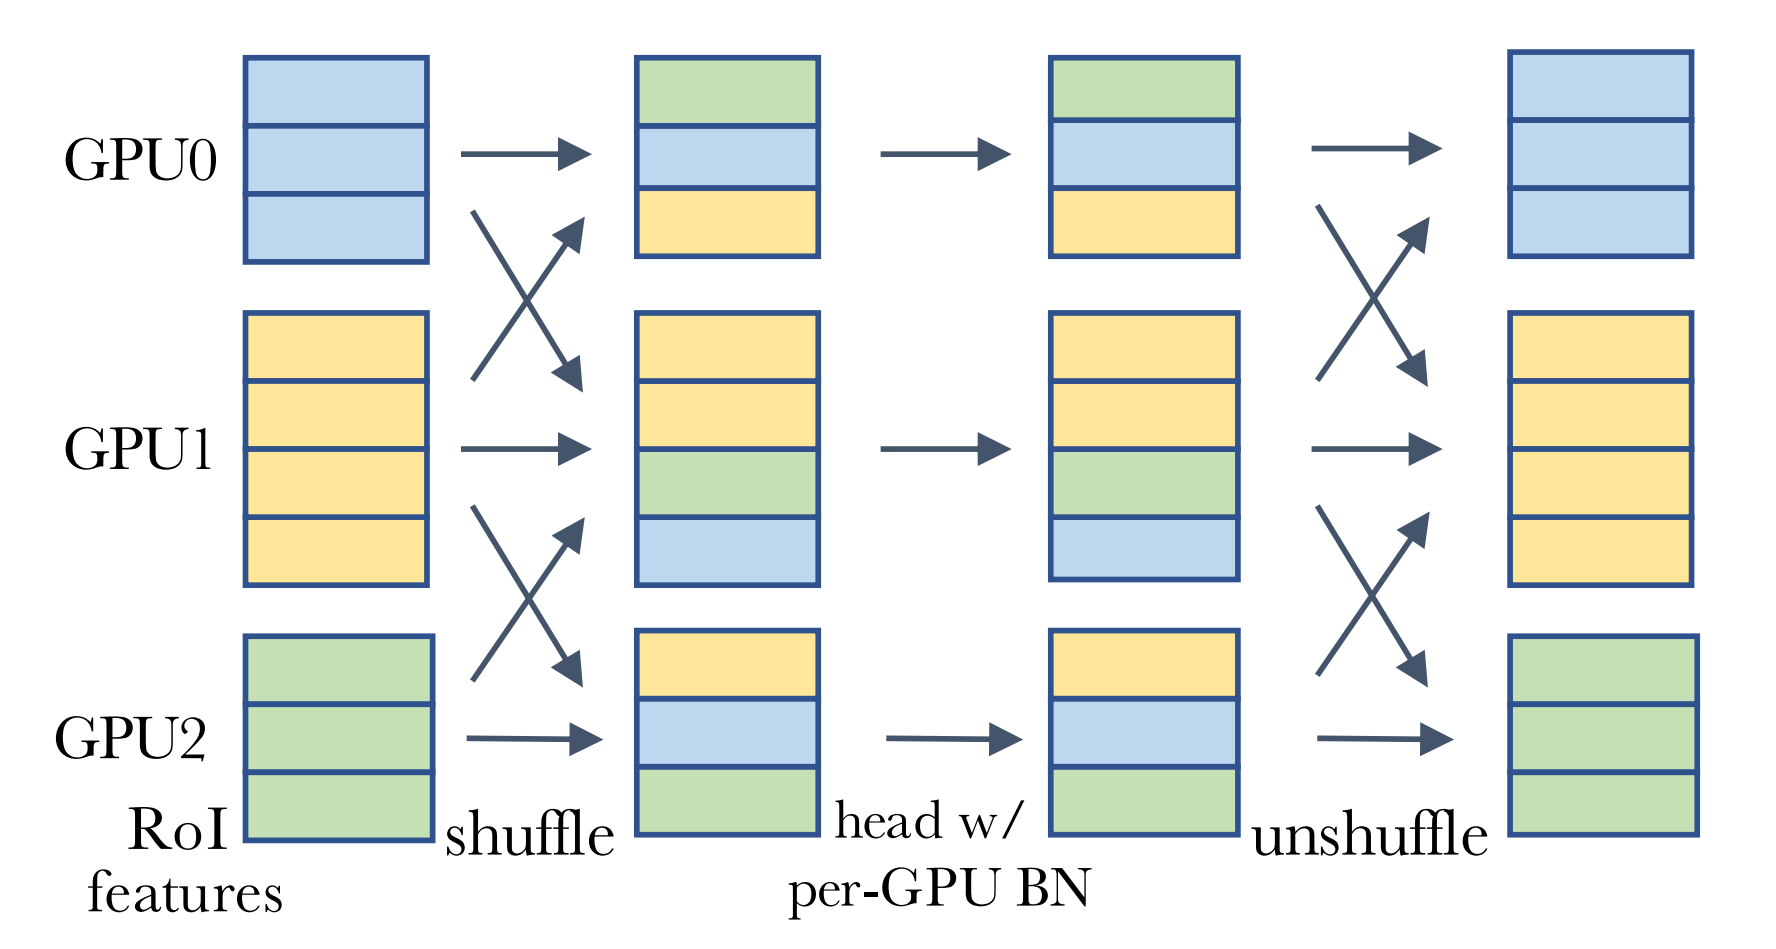
\includegraphics[width=\linewidth]{figures/shufflebn.png}
    \caption{多GPU间的交换批标准化层的示意图~\citep{wu2021rethinking}}
    \label{fig:shufflebn}
\end{figure}

随着无监督预训练的兴起,无监督学习中BatchNorm的不足也开始成为研究人员的关注点。He等人的工作~\citep{he2020momentum}认为,基于对比学习的无监督学习会在同一个batch的数据内部进行对比,而传统的BatchNorm由于在batch内部进行
标准化,会产生一定程度的信息泄露,使得模型容易通过“作弊”找到一种损失函数较小的解,影响模型最终的效果。因此他们提出了交换批标准化(Shuffling Batch Normalization),先交换当前mini-batch内
样本的顺序在进行标准化,最后再将样本顺序复原。他们设计的实验也证实了,在以对比学习为主的无监督学习中,使用交换批标准化能够显著提升最终的效果。

同样的,在Wu等人的工作中~\citep{wu2021rethinking}也提出了这一观点,以多GPU训练的Mask R-CNN模型为例,在预测头中使用标准的BatchNorm会导致结果的下降,这是由于同一个预测头中的样本往往来自同一张图片
的兴趣区域(Region of Interest,ROI),彼此之前存在信息泄露。一种解决方法便是将ROI特征在不同的GPU之间进行交换打散,使得每一个GPU上进行标准化的样本都是全体样本中的一个随机子集,降低了同一个batch内
数据的相关性,图~\ref{fig:shufflebn}为多GPU间的交换批标准化的示意图。

受到这些工作的启发,本文认为标准化层在许多实际应用场景中依然有很大的改进和提升空间,值得进行深入的研究与实验。

% !TeX root = ../thuthesis-example.tex
\chapter{随机标准化层}

\section{引言}
本章主要介绍随机标准化层(Stochastic Normalization,StochNorm)的设计思路、具体实现,并且选择少量数据的模型微调场景下进行了相关的实验。

少量数据的模型微调(Small-scale Model Fine-tune)是模型微调中的一个分支,主要的特点在于类别较多、每一类约有10到50条标注数据。
少量数据的模型微调相比小样本学习(Few-shot Learning)来说,每一类的样本数更多,训练得更加充分,得到的模型往往一定程度上能够较好地解决问题;而全量的模型微调中,一般会要求每一类的标注数据足够多,往往多于100条,
这样规模的数据虽然能够使模型获得更好的效果,但是在很多实际场景,如医疗影像数据、工业生产数据的图像识别任务,在训练前期无法获得如此多高质量的标注数据。

如何只利用一定量的高质量标注数据,就能通过模型微调得到效果较为理想的深度学习模型,正是少量数据的模型微调任务所要解决的问题,具有很高的应用价值。同时,在数据量不够充足的情况下,模型微调中存在的很多问题,诸如
灾难性遗忘、负迁移、过拟合、置信度过高等都会愈发严重,因此以少量数据的模型微调场景作为切入点,也具有很高的学术价值。


\section{相关知识}

\subsection{BatchNorm的原理}

BatchNorm在提出之时,作者认为,通过引入这种标准化的机制,能够有效减少深度神经网络的内部协变量偏移(Internal Covariate Shift,ICS)~\citep{ioffe2015BN}。由于深度神经网络涉及到在深度方向多种非线性层的叠加,每一层
的参数更新都会导致输出的数据分布发生变化。由于模型的叠加效应,在网络深处的数据分布变化会变得十分剧烈,因而会使得深度神经网络的训练随着深度的增加变得困难。而在加入BatchNorm之后,每一层输入的数据
会先进行减均值除方差的操作,得到均值为$0$方差为$1$的分布,再通过一组可学习的参数$\beta$和$\gamma$来对数据进行缩放和平移,因此BatchNorm能够动态地调整每一层数据的分布,从而一定程度上避免出现
内部协变量偏移的问题。

随着BatchNorm在深度神经网络中获得巨大的成功,越来越多的人也开始认同BatchNorm通过重参数化(reparameterize)稳定每一层网络的输出来提高网络的性能。然而,学术界一直没有非常完善的实验证明内部协变量偏移
与最终模型效果之间是否有直接的关系,以及BatchNorm是否真的缓解了内部协变量偏移的问题。

\begin{figure}
  \centering
  \subcaptionbox{损失函数Landscape}
    {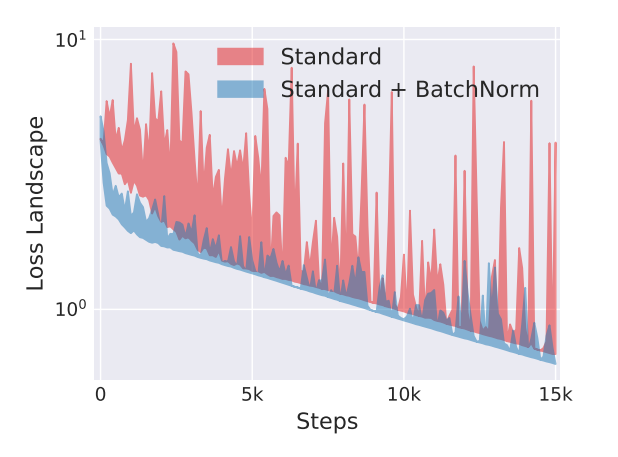
\includegraphics[width=0.46\linewidth]{figures/landscape.png}}
  \subcaptionbox{梯度的可预测性}
    {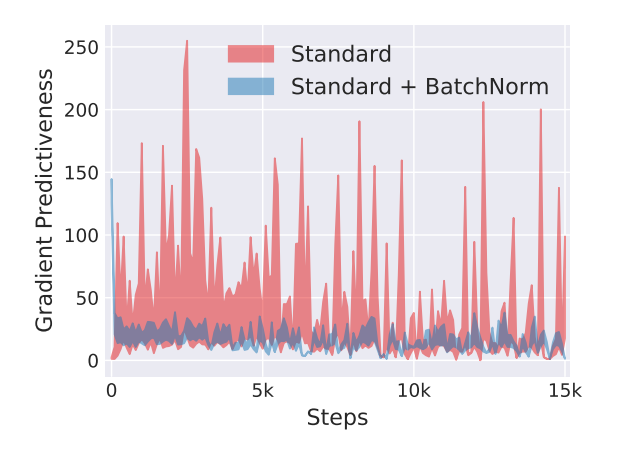
\includegraphics[width=0.47\linewidth]{figures/gradient.png}}
  \caption{BatchNorm对深度神经网络的影响~\citep{santurkar2018does}}
  \label{fig:landsacpe}
\end{figure}

Santurkar~\citep{santurkar2018does}等人的工作通过实验证明,内部协变量偏移与模型最终的效果之间没有必然的联系。作者在原本的BatchNorm的输出后加入了额外的噪声干扰,这些噪声在每一次训练迭代中都
重新生成,因此深度神经网络中每一层在每一个迭代中都有着完全不同的分布。但是添加了噪声之后的模型效果与不添加噪声的对照组相比,并没有明显的变化。同时作者也基于$L_2$距离和余弦距离计算了网络层的
协变量偏移值,发现BatchNorm的引入不会降低,甚至会增加内部协变量偏移值。这些实验证明了,内部协变量偏移与模型的性能没有直接关系,以及BatchNorm并不能显著减少内部协变量偏移。

Shibani Santurkar等人通过理论分析证明,BatchNorm的引入对深度神经网络起到了平滑(Smooth)的作用,使得网络的优化问题对应的空间地貌(landscape)更加平滑,这种影响体现在提升了损失函数的利普希茨性,
获得了更小的利普希茨(Lipschitz)常数:

\begin{definition}[利普希茨常数]
  对于在实数集的子集上定义的映射$f:D \subseteq \mathbb{R} \rightarrow \mathbb{R}$,若存在常数$K$,使得$|f(a)-f(b)| \leq K|a-b| \quad \forall a,b \in D$,则称$f$符合利普希茨条件,
  对于$f$最小的常数$K$成为$f$的利普希茨常数。
\end{definition}

BatchNorm的重参数化使得深度神经网络损失函数对应的梯度的利普希茨常数更小,使得其更加稳定可靠。图~\ref{fig:landsacpe}展示了深度神经网络在加入BatchNorm之后的在损失函数Landscape和梯度可预测性(即
沿着梯度方向梯度的变化值)上的变化。
利普希茨性更好的梯度,使得基于梯度的优化算法能够使用更大的步长进行探索,而不至于发生损失函数突然骤变的现象,例如极其平坦的区域(梯度消失)或尖锐的局部极值(梯度爆炸)。这种性质加速了深度神经网络的训
练,也使其对于学习率等超参数的选择不再那么敏感,从而更容易获得更好的效果。


\subsection{基于正则化的模型微调}
\label{section:regularize}
相比BatchNorm这种从网络结构上进行的正则化约束来说,主流的模型微调方法往往通过在损失函数中加入显式的正则化约束项来进行,以分类任务为例,可以用一个通用的损失函数描述:

\begin{equation}
\label{equal-finetune}
	\mathop {\min} \limits_{ F_{\symup{\Theta}}, G_{\symup{\Theta}}} \sum\limits_{i = 1}^n {\texttt{Loss}(G(F(x_i;F_{\symup{\Theta}});G_{\symup{\Theta}}),y_i)}  + \texttt{Reg} (\cdot)
\end{equation}

其中$x$和$y$表示数据和对应的标签,$F$和$G$分别表示预训练的特征提取器和分类器,$F_{\symup{\Theta}}$和$G_{\symup{\Theta}}$分别表示各自的网络参数,$\texttt{Loss} (\cdot)$表示损失函数,$\texttt{Reg} (\cdot)$表示正则项。
而不同模型微调方法的主要差异则在于对正则项$\texttt{Reg} (\cdot)$的设计,例如如何更大程度利用预训练模型中的知识来设计约束项,从而避免在小的目标域数据集上发生过拟合。

\textbf{$\bm{L_p}$约束 } $L_p$约束中使用模型参数的$L_p$范数作为约束项,是最为经典的一种正则化方法。$L_p$范数的定义如下:

\begin{definition}[$L_p$范数]
  对于$\vec{x}=(x_1, x_2, \cdots ,x_n) \in \mathbb{R}^n$,则$\vec{x}$的$L_p$范数$L_p(\vec{x})={\vert\vert \vec{x} \vert\vert}_p = (\sum_{i=1}^n {\vert x_i \vert}^p)^{\frac{1}{p}} \quad p \geq 1 $
\end{definition}

在深度学习中,一般使用$L_1$和$L_2$范数作为约束项,使用$L_1$范数能够使得深度神经网络获得更好的稀疏性,而模型微调领域中一般使用$L_2$范数:

\begin{equation}
  \texttt{Reg} (F_{\symup{\Theta}}, G_{\symup{\Theta}}) = \frac{1}{\alpha} (\vert\vert F_{\symup{\Theta}} \vert\vert_2^2 + \vert\vert G_{\symup{\Theta}} \vert\vert_2^2) \quad \alpha \in \mathbb{R}
\end{equation}

\textbf{$\bm{L_2}$-SP } $L_2$-SP的目标是缓解模型微调中的灾难性遗忘问题,通过在$L_2$的基础上加入对特征提取器网络参数的约束来实现:

\begin{equation}
  \texttt{Reg} (F_{\symup{\Theta}}, G_{\symup{\Theta}}) = \frac{1}{\alpha} (\vert\vert F_{\symup{\Theta}} \vert\vert_2^2 + \vert\vert G_{\symup{\Theta}} \vert\vert_2^2) + \frac{1}{\beta} \vert\vert F_{\symup{\Theta}} - F_{{\symup{\Theta}}_0} \vert\vert_2^2 \quad \alpha, \beta \in \mathbb{R}
\end{equation}

其中$F_{\symup{\Theta}}$表示特征提取器当前的网络参数,$F_{{\symup{\Theta}}_0}$则表示在预训练模型中特征提取器的网络参数。$L_2$-SP在对网络整体参数做出正则化约束的同时,还迫使特征提取器的参数与预训练模型中不要差异
过大,从而一定程度上避免灾难性遗忘的发生。

\textbf{DELTA } 相较于前面两种作用于网络参数的正则化方法来说,$\rm{DELTA}$则更侧重对深度神经网络获得的特征表征(representation)进行约束,通过引入注意力机制对网络的特征图在特定层进行筛选,对具有更好
迁移性的特征通道赋予更高的注意力权重,第$j$个通道的注意力权重为:


\begin{equation}
\begin{aligned}
  A_j(G,F,F_{{\symup{\Theta}}_0},x_i,y_i) = &\texttt{softmax} (\texttt{Loss}(G(F(x_i; F_{{{\symup{\Theta}}_0}\backslash j});G_{{{\symup{\Theta}}_0}\backslash j}), y_i) \\ 
  &-\texttt{Loss}(G(F(x_i; F_{{\symup{\Theta}}_0});G_{{\symup{\Theta}}_0}), y_i)) \\
\end{aligned}
\end{equation}

其中$F_{{{\symup{\Theta}}_0}\backslash j}$和$G_{{{\symup{\Theta}}_0}\backslash j}$表示去除第$j$个通道网络参数的特征提取器和分类器,最终的正则化约束项为:

\begin{equation}
\begin{aligned}
  \texttt{Reg} (F_{\symup{\Theta}}, G_{\symup{\Theta}}) &= \frac{1}{\alpha} (\vert\vert F_{\symup{\Theta}} \vert\vert_2^2 + \vert\vert G_{\symup{\Theta}} \vert\vert_2^2) + \frac{1}{\beta} \sum_{i=1}^{m}\sum_{j=1}^{N} { 
    A_j(G,F,F_{{\symup{\Theta}}_0},x_i,y_i) \texttt{Reg}(f_j)}  \\
    \texttt{Reg}(f_j) &= \vert\vert f_j(F,F_{{\symup{\Theta}}}, x_i) - f_j(F,F_{{\symup{\Theta}}_0},x_i) \vert\vert_2^2 \quad \alpha, \beta \in \mathbb{R} \\
\end{aligned}
\end{equation}

其中$f_j$表示网络特定层输出特征图的第$j$个通道。

\textbf{BSS } 尽管模型微调场景下大多数的正则化方法都是针对灾难性遗忘问题而提出,也有一部分工作面向负迁移(Negative Transfer)问题。BSS(Batch Spectral Shrinkage)~\citep{chen2019catastrophic}
中参考主角(Principal Angles)分析提出了一致角(Corresponding Angles)的概念,通过度量两个矩阵的特征向量之间的余弦距离,来刻画特征图矩阵不同特征向量的迁移性,即不同领域间一致角越小的特征向量具有越好
的迁移性。BSS首先对特征提取器输出的特征进行奇异值分解(Singular Value Decomposition,SVD):
\begin{equation}
  F(\symbf{x}) = \symbf{\symup{U\Sigma V^\top}}
  % \symbf{\symup{\Sigma}} &= (\sigma_1, \sigma_2, \cdots, \sigma_n) \\
\end{equation}

之后基于分解得到的奇异值对网络的训练进行正则化约束:

\begin{equation}
  \texttt{Reg} (\cdot) = \alpha \sum_{i=1}^k \sigma_{-i}^2 \quad \alpha \in \mathbb{R} \\
\end{equation}

其中$k$表示要进行约束的奇异值的数量,而$\sigma_{-i}$表示第$i$小的奇异值。

总的来说,正则项$\texttt{Reg} (\cdot)$的引入更偏向于一种强制性的约束,迫使深度神经网络的训练满足某种条件,从而一定程度上避免在模型微调中遇到的灾难性遗忘或者负迁移的问题。
但是这些约束条件往往需要进行巧妙的设计,同时使用一定的超参数与原始的损失函数进行权衡,否则会对网络的训练产生过大的影响,甚至带来负面的影响。

\section{随机标准化层}

本文提出的随机标准化层(Stochastic Normalization)是以深度神经网络中使用非常广泛的BatchNorm为基础,通过引入双分支结构和随机前馈机制设计的新的标准化层结构。

\subsection{BatchNorm在模型微调中的不足}

尽管BatchNorm被广泛应用在深度神经网络中,它依然存在着很多的缺陷。在训练阶段,BatchNorm的输出依赖于这一批数据的均值和方差,而真正用于估计数据分布的期望和方差的$\tilde{\mu}$和$\tilde{\sigma}^2$则只在推理阶段被使用。这意味着
包含BatchNorm的深度神经网络的训练容易过分依赖批数据的期望和方差,从而影响网络泛化性。尤其在训练样本总数较少或者每一批数据内部差异较小的情况下,这一批数据的均值和方差会存在较大的误差。


BatchNorm目前被广泛应用于各种深度神经网络结构的训练当中,在数据量以及Batch Size都足够大的情况下,往往能取得非常好的效果。这是由于足够大的Batch Size能够使BatchNorm中用于训练阶段标准化的统计量
$\mu$和$\sigma^{2}$更加准确可靠,而足够大的数据量能够使用于预测阶段标准化的统计量$\tilde{\mu}$和$\tilde{\sigma}^{2}$更好地估计整体数据分布的期望和方差,两个条件的满足保证了BatchNorm的效果。
在物体检测领域中,由于GPU计算能力以及显存的限制,Batch Size往往只有个位数,此时$\mu$和$\sigma^{2}$的估计就容易产生较大误差,因此一般使用改进的Batch Norm或者换用其他标准化层。

而在图像分类任务中,常规的GPU显存足以容纳足够大的Batch Size用于训练,因此前者的估计依然得以保证,但是在模型微调场景下往往只有很少量的有标注数据,相比起预训练阶段要少得多,导致$\tilde{\mu}$和$\tilde{\sigma}^{2}$
的估计容易出现偏差,考虑到BatchNorm在推理阶段使用这两个估计值来估计数据分布的期望和方差,BatchNorm很容易在一些模型微调场景下无法获得很好的效果。

除此之外,相较于常规的从头训练而言,预训练模型在模型微调场景中的作用不可忽视。但是在传统的模型微调场景下,深度神经网络会使用预训练模型的网络参数进行初始化,但是一般只包括特征提取器中的可学习参数,
而BatchNorm中的$\tilde{\mu}$和$\tilde{\sigma}^{2}$则是通过滑动平均的方式进行更新的得到的,属于不可学习的统计量,因此在模型微调时,预训练模型在预训练数据上更新得到的$\tilde{\mu}$和$\tilde{\sigma}^{2}$
会被直接丢弃。但是对于基本收敛的预训练模型而言,每一层网络层的输入输出与BatchNorm的标准化过程相互耦合,如果直接丢弃这些滑动平均的统计值,便无法充分利用预训练模型中的知识,往往会在训练初期导致
可学习参数与BatchNorm之间的不匹配(mismatch)。

% 在节~\ref{section:problem}中提到的

% BatchNorm目前被广泛应用于各种深度神经网络结构的训练当中,在数据量$n$以及Batch Size$m$都足够大的情况下,往往能取得非常好的效果。这是由于足够大的$m$能够使BatchNorm中的
% $(\mu, \sigma^{2})$更加准确可靠,而足够大的$n$能够使$(\tilde{\mu}, \tilde{\sigma}^{2})$更好的估计数据分布$P$的期望和方差,
% 但是Batch Size $m$往往依赖于图形处理器(Graph Processing Unit,GPU)的计算能力以及显存,在很多实际场景中并不会很大,例如在物体检测(Object Detection)中,单张图形处理器上
% 的Batch Size $m$一般很难超过$10$。而在图像分类(Image Classification)任务中,$m$往往是几十甚至几百,因此BatchNorm可以很好地对$(\mu, \sigma^{2})$进行计算。但是在模型微调
% 场景下,数据量$n$相比起预训练阶段来说要小得多,如果数据量不够充足,往往BatchNorm无法获得很好的效果。

\subsection{双分支结构}

为了解决上一节提到的BatchNorm在模型微调场景下存在的问题,我们将标准化的过程分为两个分支,一个分支仍然使用BatchNorm的计算方式,另一个分支则使用网络当前估计得到的$\tilde{\mu}$和方差$\tilde{\sigma}^2$来进行标准化:
\begin{equation}
  \label{equal-sn_mean&var}
  \begin{aligned}
    \widehat{x}_{i,0}=\frac{x_{i}-\tilde{\mu}}{\sqrt{\tilde{\sigma}^{2}+\epsilon}},\quad
    \widehat{x}_{i,1}=\frac{x_{i}-\mu}{\sqrt{\sigma^{2}+\epsilon}}.
  \end{aligned}
\end{equation}

\begin{figure}
  \centering
  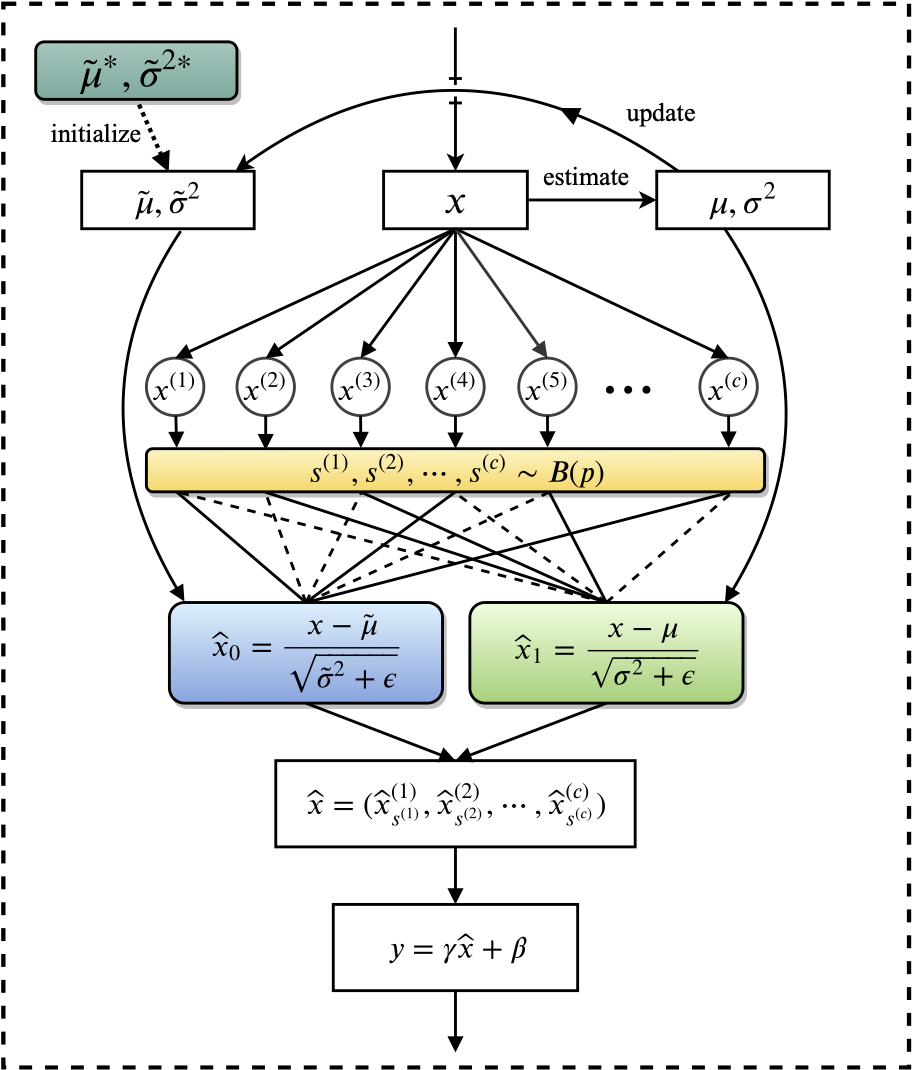
\includegraphics[width=0.7\linewidth]{figures/arch.png}
  \caption{StochNorm的整体结构}
  \label{fig:arch}
\end{figure}

下一步是基于某个概率$p$对两个分支对特征图进行标准化的结果进行选择。令$s$表示最终选择的分支,则$x_{i,s}$表示传入下一步的标准化特征图。本文采用伯努利分布(Bernoulli Distribution)

\begin{equation}
  P(s)=\left\{
  \begin{matrix}
    p, & s=1\\ 
    1-p,  & s=0
  \end{matrix}
  \right.
\end{equation}

对两个分支的标准化结果进行随机选择,这一选择的过程可以表示为:

\begin{equation}
  \widehat{x}_{i}=(1-s)\widehat{x}_{i,0}+s\widehat{x}_{i,1}
\end{equation}

之后依旧按照BatchNorm的操作,使用参数$\beta$和$\gamma$对$\widehat{x}_{i}$进行缩放的平移。

通过伯努利分布的概率$p$,我们可以根据实际场景来平衡个分支的输出。当$p=1$时,StochNorm退化为BatchNorm,但是当训练数据较少时,传统的基于BatchNorm的训练很容易出现过拟合;而$p=0$时,会完全依赖滑动平均估计的统计值进行标准化,
即使在输入数据统计值有明显差异的情况下,依旧会强迫深度神经网络根据滑动平均估计得到的均值和方差进行标准化。但是通过引入随机选择的机制,StochNorm能够让网络在训练过程中,既不会完全忽视输入数据的统计特征,也不会过分拟合,这种标准化层
结构以一种类似Dropout~citep{}的方式对深度神经网络的训练实现了正则化约束,从而一定程度上避免了过拟合的发生,提升了模型的效果。

StochNorm的整体结构如图~\ref{fig:arch}所示,其中$c$表示输入的特征图$x$的通道数,$j$表示通道的小标,$\tilde{\mu}^*, \tilde{\sigma}^{2^*}$表示预训练模型中的滑动平均估计的统计值。在推理阶段,黄色和绿色的模块将不被使用。StochNorm的具体的计算过程如算法~\ref{alg:main}所示。

\subsection{更充分地利用预训练模型参数}

% 统计量和模型网络的耦合

在节~\ref{section:bn}中提到,BatchNorm中的$\tilde{\mu}, \tilde{\sigma}^2$对实际的网络训练过程没有影响。因此尽管在预训练模型中也保存了过去更新得到的$\tilde{\mu}^*, \tilde{\sigma}^{2^*}$,
由于BatchNorm的机制,这些参数对模型微调阶段没有帮助。同时,由于BatchNorm中使用滑动平均的方式对两个估计值进行更新,初始值的影响也随着训练的进行不断减小。尽管并非是可学习的网络参数,
$\tilde{\mu}, \tilde{\sigma}^2$也是通过预训练数据,以及预训练数据上学习得到的可学习网络参数计算得到的,理所当然地包含着许多预训练数据中有价值的知识,但是现有的方法中直接忽略了这些知识。

在StochNorm中,由于双分支结构的巧妙设计,存在着一支使用$\tilde{\mu}, \tilde{\sigma}^2$进行标准化的分支,可以自然而然地使用$\tilde{\mu}^*, \tilde{\sigma}^{2^*}$作为其初始值,如图~\ref{fig:arch}中
左上角所示。通过这种方式,StochNorm使得预训练模型中的滑动平均估计的统计值也能够参与训练,对模型微调的最终效果起到帮助。这种初始化的策略也对网络的训练起到了隐式的正则化约束。

\begin{algorithm}[htbp]
  \caption{随机标准化层 (StochNorm)}
  \label{alg:main}
  \begin{algorithmic}
      \STATE \hspace{-11pt} {\bfseries 输入}: 一批数据内每个通道的特征图 $x=\{x_{i}\}_{i=1}^{m}$;\\
      (BatchNorm) 滑动平均更新速率 $\alpha \in (0,1)$ 和可学习参数 $\beta, \gamma$;\\
      (StochNorm) 滑动平均估计的统计值 $\tilde{\mu}, \tilde{\sigma}^2$ (初始值为 $\tilde{\mu}^*, \tilde{\sigma}^{2^*}$) 和分支选取概率 $p \in (0,1)$。 \\
      \STATE \hspace{-11pt} {\bfseries 输出}: $y={\textrm{StochNorm}}(x)$.。
  
      \STATE \hspace{-11pt} \textbf{训练阶段:}
      \STATE $\displaystyle \mu \leftarrow \frac{1}{m}\sum_{i=1}^{m}x_{i}, \quad \sigma^2 \leftarrow \frac{1}{m}\sum_{i=1}^{m}(x_i-\mu)^2$ \hfill $//$ \textit{计算均值和方差}
      \setstretch{1.4}
  
      \STATE $\displaystyle \widehat{x}_{i,0} \leftarrow
      \frac{x_{i}-\tilde{\mu}}{\sqrt{\tilde{\sigma}^2+ \epsilon}}$
      \hfill $//$ \textit{使用滑动平均估计的统计值进行标准化}
      
      \STATE $\displaystyle \widehat{x}_{i,1} \leftarrow 
      \frac{x_{i}-\mu}{\sqrt{\sigma^2+\epsilon}}$
      \hfill $//$ \textit{使用批数据统计值进行标准化}

      \STATE $\widehat{x}_{i}=(1-s)\widehat{x}_{i,0}+s\widehat{x}_{i,1}, \quad s \sim B(p)$
      \hfill $//$ \textit{对每个通道进行随机的分支选取}
      
      \STATE $y_{i} \leftarrow \gamma \widehat{x}_{i} +\beta$
      \hfill $//$ \textit{伸缩与平移}
      \STATE $\tilde{\mu} \leftarrow \tilde{\mu} + \alpha (\mu-\tilde{\mu}), \quad \tilde{\sigma}^2 \leftarrow \tilde{\sigma}^2 + \alpha (\sigma^2-\tilde{\sigma}^2)$ 
      \hfill $//$ \textit{滑动平均更新估计值}
      
      \STATE \hspace{-11pt} {\bfseries 推理阶段:}
      \STATE $\displaystyle y_{i} \leftarrow \gamma \frac{x_{i}-\tilde{\mu}}{\sqrt{\tilde{\sigma}^2 + \epsilon}} + \beta$ \hfill $//$ \textit{使用滑动平均估计值进行标准化}
  \end{algorithmic}
\end{algorithm}

总的来说,StochNorm从两个方面使得模型微调具有更好的鲁棒性和泛化性:双分支的结构设计加上随机选取分支进行标准化的机制,实现了两种标准化方式的结合,对模型微调阶段起到了正则化的约束效果;
将预训练模型中的非可学习参数$\tilde{\mu}^*, \tilde{\sigma}^{2^*}$利用了起来,更大程度上迁移了预训练模型中的知识。
同样的,由于在训练阶段引入了通过$\tilde{\mu}^*, \tilde{\sigma}^{2^*}$进行标准化的分支,StochNorm进一步缓解了在节~\ref{section:problem}中提到的训练和预测阶段标准化方式不一致导致的问题。 


% \begin{itemize}
%   \item 双分支的结构设计加上随机选取分支进行标准化的机制,实现了两种标准化方式的结合,对模型微调阶段起到了正则化的约束效果;
%   \item 将预训练模型中的非可学习参数$\tilde{\mu}^*, \tilde{\sigma}^{2^*}$利用了起来,更大程度上迁移了预训练模型中的知识。
% \end{itemize}



\subsection{使用随机标准化层进行模型微调}

本节介绍StochNorm的主要应用方式和场景,包括与其他主流模型微调方法或者深度神经网络结构相结合,进一步提升模型微调的效果。

\textbf{与主流模型微调方法相结合 } 在节~\ref{section:regularize}中提到的,主流的基于正则项的模型微调方法,一般会在模型层面外,对训练时的损失函数进行修改,而且更偏向于一种显式的目的性较强的约束。
StochNorm则通过结构上的巧妙设计,隐式地提升了深度神经网络的迁移能力,同时起到正则化约束的效果。这两种方式是相互正交、相互补充的,通过将特征提取器$F$中的BatchNorm替换为StochNorm,
便可以同时获得两种正则化效果,进一步提升模型的最终效果,在节~\ref{section:ablation}中有更详细的实验验证。

\textbf{与主流深度神经网络结构相结合 } 作为一种通用并且轻量的标准化层结构,StochNorm可以被非常轻松地加入各种主流的使用了BatchNorm的深度神经网络结构中,只需要直接将BatchNorm替换为StochNorm即可。
如图~\ref{fig:integratio}所示,StochNorm可以应用在多种主流深度神经网络结构中,如VGG-16~\citep{simonyan2015very},ResNet~\citep{he2016deep}以及Inception Net~\citep{szegedy2016rethinking},
而不需要修改其他组件。

\begin{figure}
  \centering
  \subcaptionbox{VGG Block}
    {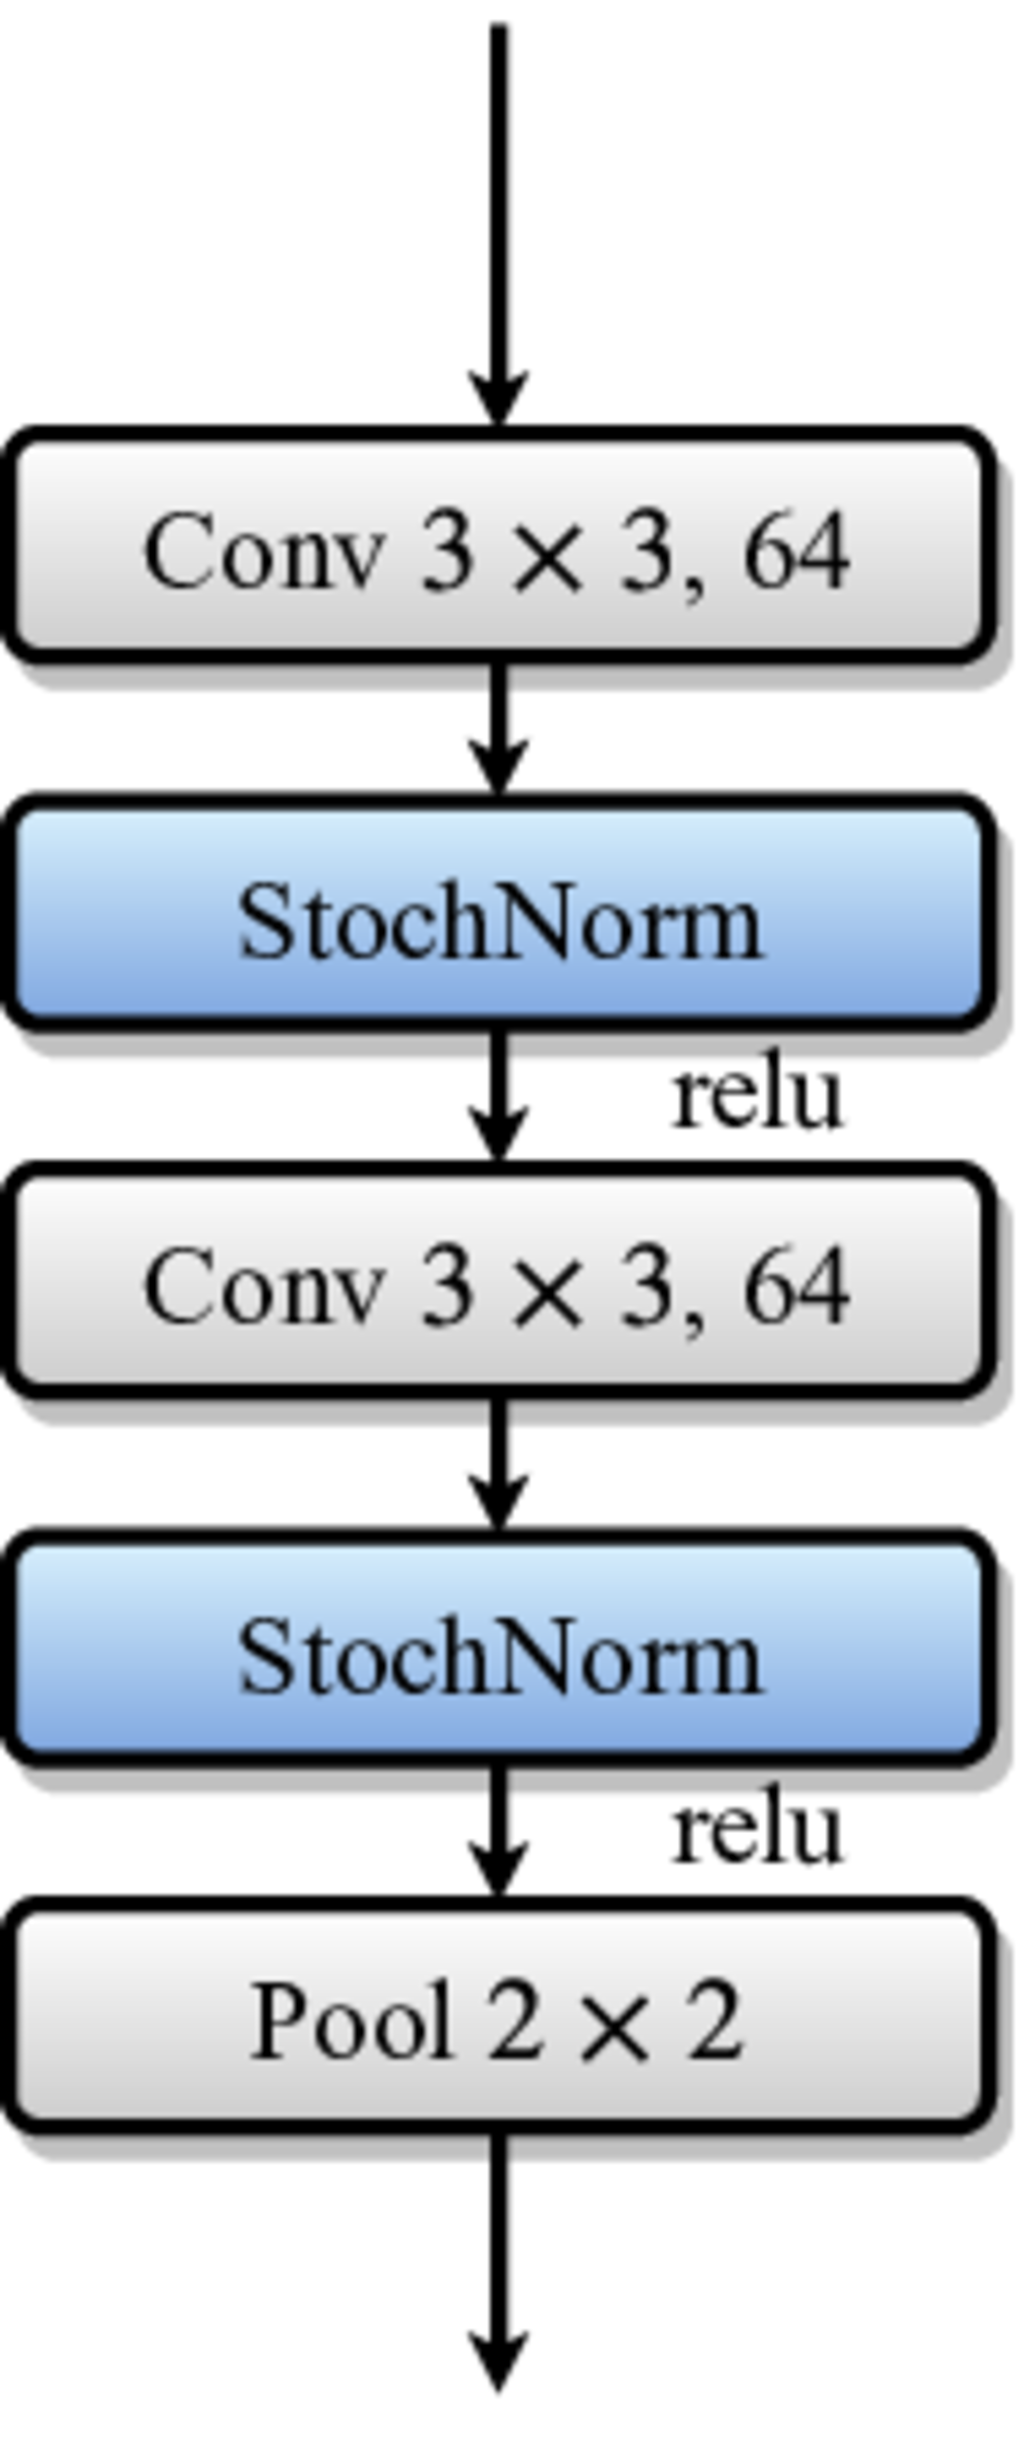
\includegraphics[width=0.16\linewidth]{figures/vgg-block.png}}
  \hspace{15pt}
  \subcaptionbox{Residual Block}
    {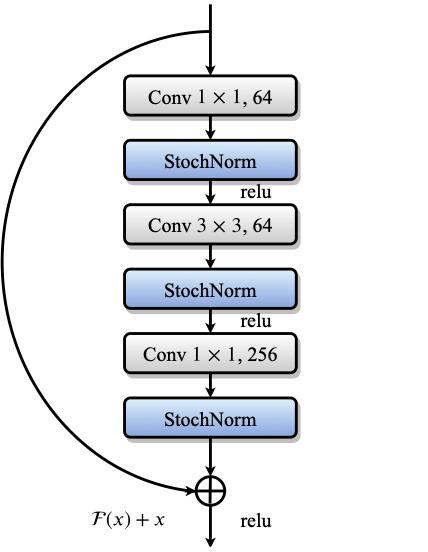
\includegraphics[width=0.29\linewidth]{figures/resnet-block.png}}
  \subcaptionbox{Inception Block}
    {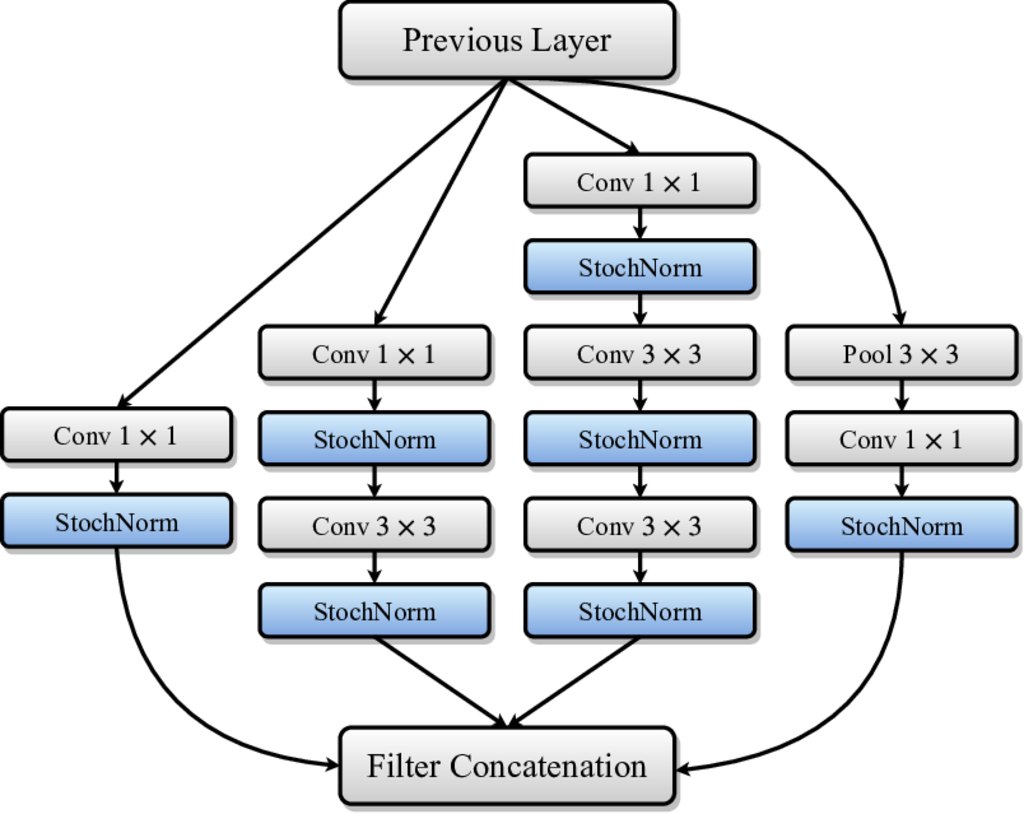
\includegraphics[width=0.44\linewidth]{figures/inception-block.png}}
  \caption{在主流深度神经网络结构中使用StochNorm}
  \label{fig:integratio}
\end{figure}


\section{实验}

\subsection{实验设计}
\label{section:settings}

\textbf{深度学习框架 } 随着深度学习的不断发展,研究人员们也相应开发了各式各样的深度学习框架,逐渐成为了深度学习不可或缺的一部分。目前学术界主流的深度学习框架为TensorFlow[引]和PyTorch\citep{benoit_pytorch:_2019}。
PyTorch使用了动态的计算图,使用方法很接近原生的Python语言,具有效率高、可读性强等优点,逐渐成为学术界使用最为广泛的深度学习框架。因此本文使用PyTorch来进行相关的实验。

\textbf{实验环境 } 本文的所有实验均使用装有8块GPU的深度学习服务器来进行,服务器的详细配置如表~\ref{table:server-setting}所示。

\begin{table*}[h]
	\begin{center}
	\caption{服务器配置信息}
	\label{table:server-setting}
    \begin{tabular}{ll}
        \toprule
        项目 & 配置信息 \\
        \midrule
        操作系统 & Ubuntu 18.04.3 LTS \\
        中央处理器 & Intel(R) Xeon(R) Gold 6130 CPU @ 2.10GHz \\
        中央处理器核心数 & 64 \\
        内存 & 32GB \\
        图形处理器 & NVIDIA TITAN X \\
        显存 & 12GB \\
        Python版本 & 3.8.10 \\
        PyTorch版本 & 1.9.0 \\
        CUDA版本 & 11.2 \\
        \bottomrule
    \end{tabular}
	\end{center}
\end{table*}

\textbf{数据集 } 本文在三个细粒度分类数据集上进行了模型微调相关的实验:\textbf{CUB-200-2011 }~\citep{WelinderEtal2010}是一个鸟类图片的细粒度分类数据集,包含一共$200$种鸟类,共$11788$张图片,是CUB-200数据集
的扩展版本;\textbf{Standford Cars }~\citep{KrauseStarkDengFei-Fei_3DRR2013}是一个车辆图片的细粒度分类数据集,包含一共$196$种车辆,共$16185$张图片;\textbf{FGVC Aircraft }~\citep{maji2013fine}是一个航空飞行器的细粒度分类数据集,包含$102$种飞行器,共$10200$张
图片。三个数据集的部分图片如图~\ref{fig:datasets}所示。可以看出,三个数据集都属于同一大类下不同细分类别的图像分类问题,具有图片规模较小、类间差异较小等特点,很适合作为验证模型微调方法的评测数据集。

\begin{figure}
  \centering
  \subcaptionbox{CUB-200-2011}{
    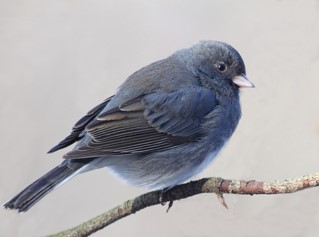
\includegraphics[width=0.271\linewidth]{figures/cub/1.jpg}
    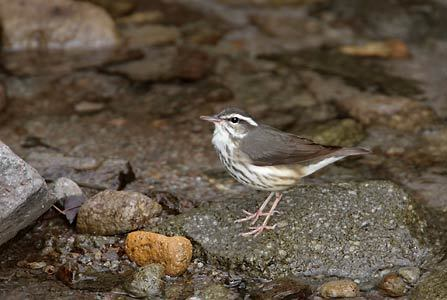
\includegraphics[width=0.3\linewidth]{figures/cub/4.jpg}
    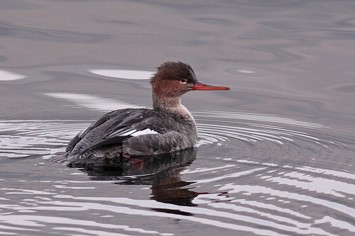
\includegraphics[width=0.305\linewidth]{figures/cub/3.jpg}
  }
  \subcaptionbox{Standford Cars}{
    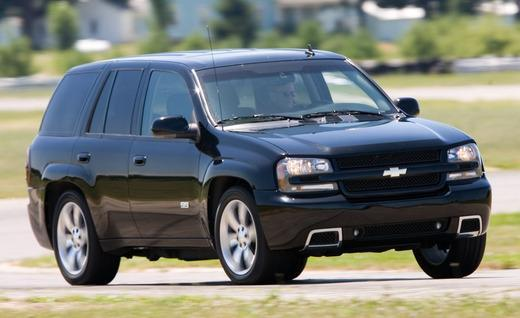
\includegraphics[width=0.3\linewidth]{figures/car/1.jpg}
    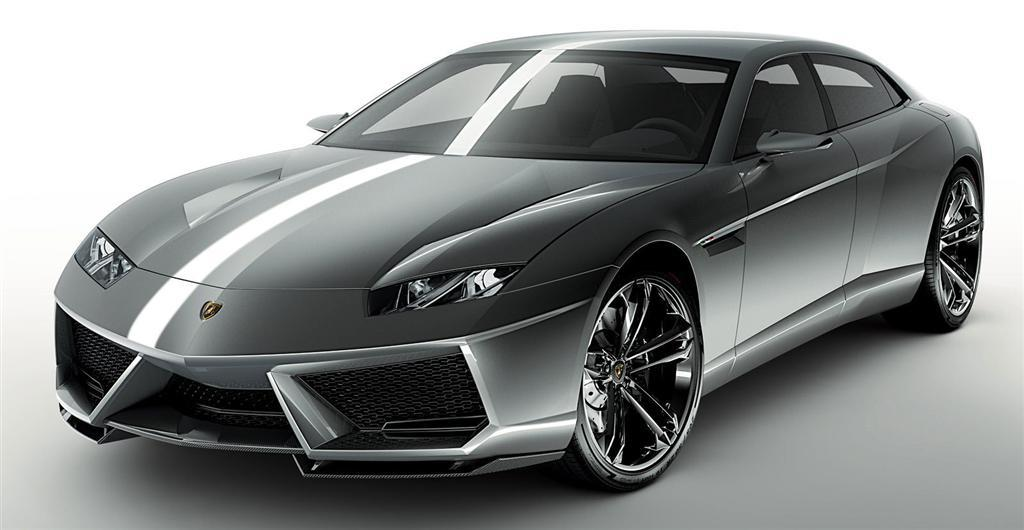
\includegraphics[width=0.3\linewidth]{figures/car/2.jpg}
    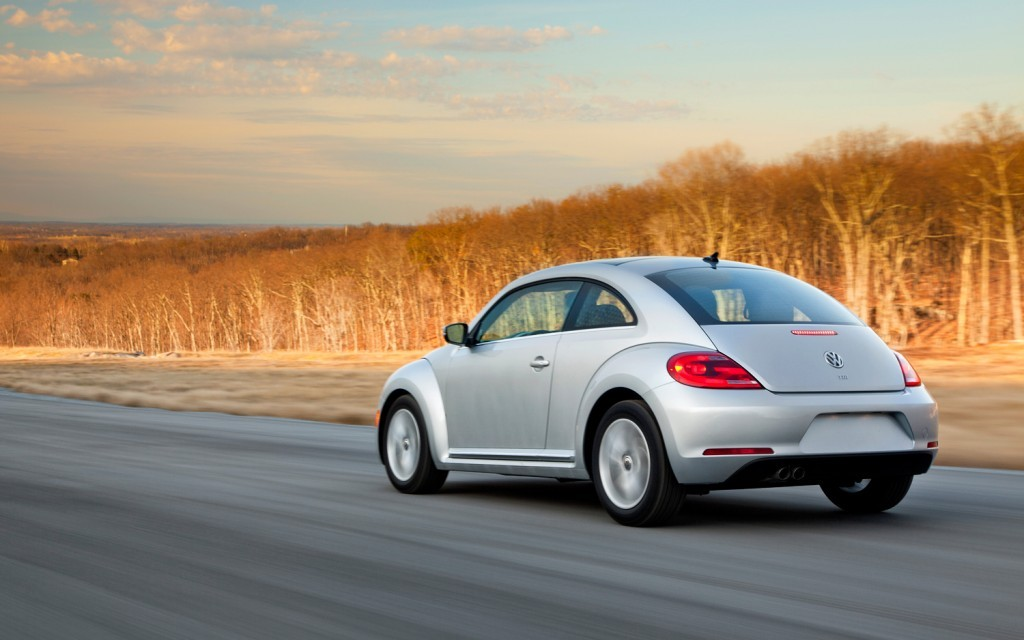
\includegraphics[width=0.3\linewidth]{figures/car/3.jpg}
  }
  \subcaptionbox{FGVC Aircraft}{
    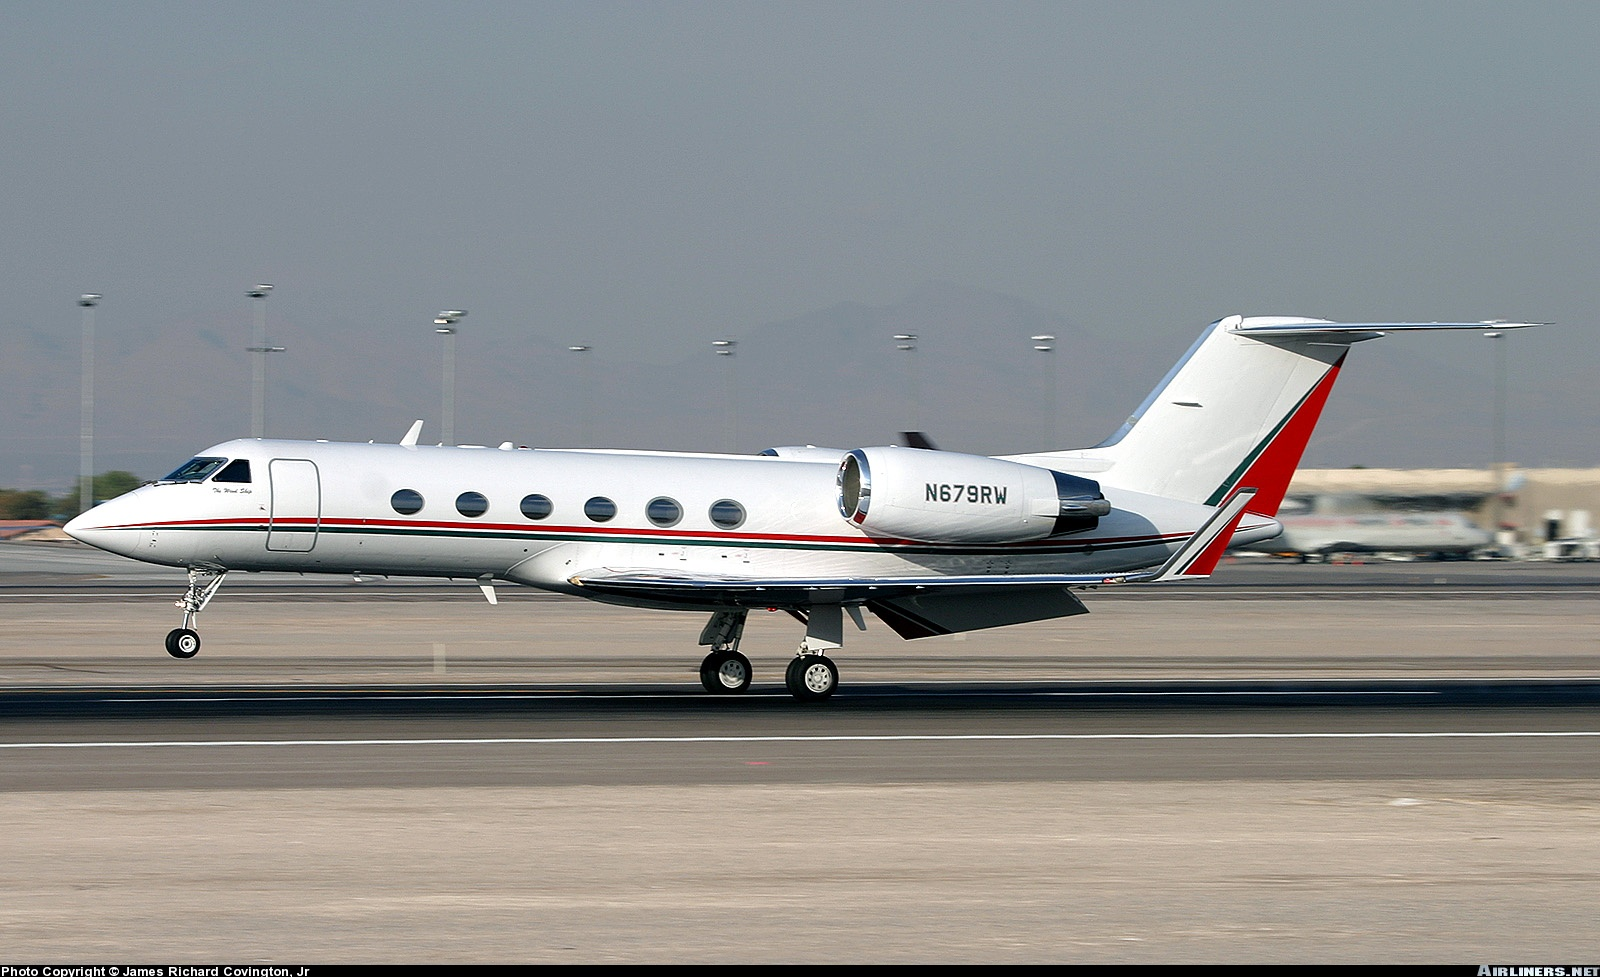
\includegraphics[width=0.335\linewidth]{figures/air/1.jpg}
    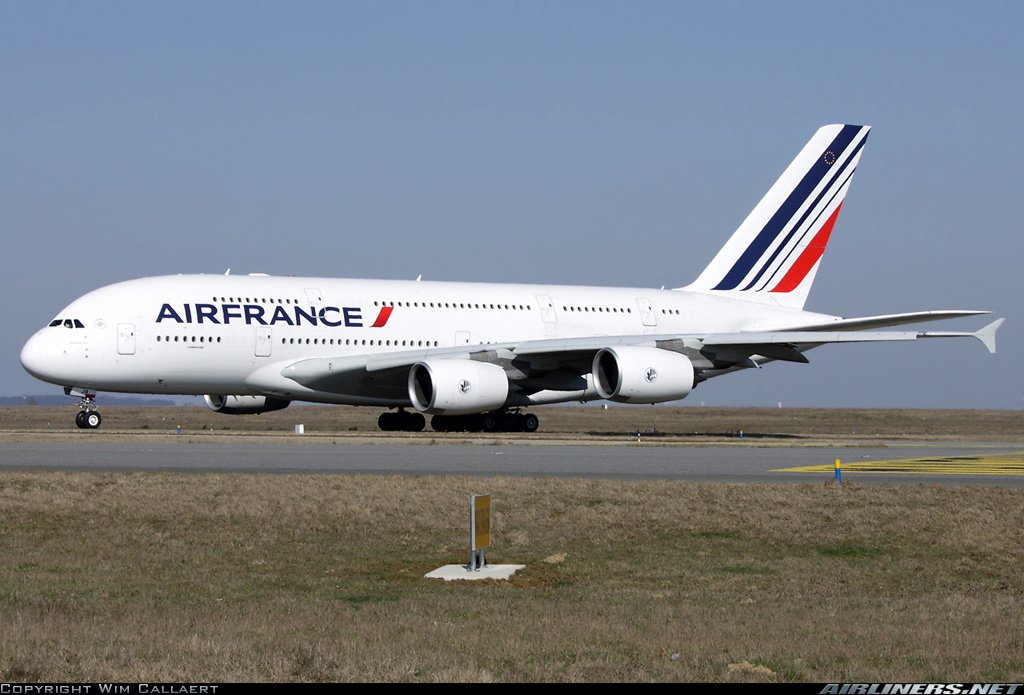
\includegraphics[width=0.3\linewidth]{figures/air/2.jpg}
    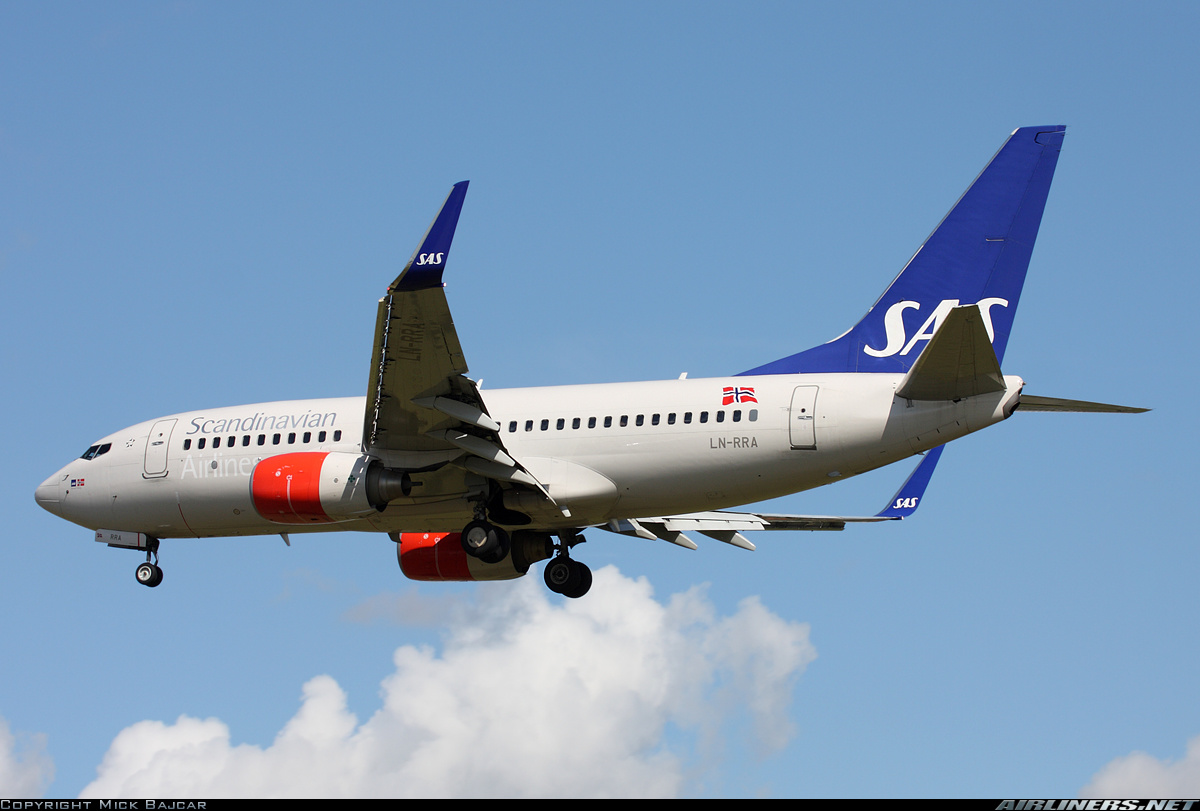
\includegraphics[width=0.3\linewidth]{figures/air/3.jpg}
  }
  \caption{数据集示例}
  \label{fig:datasets}
\end{figure}


\textbf{相比较的模型微调方法 } 为了展示随机标准化层在模型微调任务中的效果,我们选取了节~\ref{section:regularize}中的几种有代表性的模型微调方法进行比较:基线(Baseline)\textbf{$\bm{L_2}$范数},即不使用任何方法,直接利用预训练模型的参数作为初始化进行
微调训练;\textbf{$\bm{L_2}$-SP}\citep{xuhong2018explicit},通过将深度神经网络的网络参数,通过正则化的方式约束在预训练模型的网络参数附近,来缓解模型微调中容易遇到的灾难性遗忘;\textbf{DELTA}\citep{li2018delta},在特征图
维度通过一种有监督的注意力机制进行筛选,选出更适合进行模型微调的特征;\textbf{BSS}\citep{chen2019catastrophic},通过对深度神经网络生成表征的特征值进行正则化约束,来避免在模型微调中出现负迁移(Negative Transfer)。这三种方法均在发表
阶段取得了相应的模型微调任务上最好的效果,并且都能够有效地避免深度神经网络在微调阶段出现过拟合的现象。

\textbf{实验细节 } 模型微调部分的训练与验证遵循了相关工作\citep{xuhong2018explicit,li2018delta,chen2019catastrophic}中的设定,对于深度神经网络的特征提取器部分(Feature Extractor),使用预训练模型的参数作为其初始值,而对于与图像分类任务相关的最后一层
全连接层(Fully Connected Layer),则完全随机初始化从头开始训练。由于最后一层全连接层是随机初始化的,因此其学习率设为特征提取器部分的学习率的$10$倍。训练过程中本文采用随机梯度
下降(Stochasitc Gradient Descent,SGD)作为深度神经网络的优化器,动量值(Momentum)设置为$0.9$,并相应地加入了学习率衰减(Learning Rate Decay)策略。每组实验使用不同的随机种子
重复实验五次,结果取五次的平均值,并且汇报相应的标准差。对于训练数据与验证数据的划分,本文遵循了数据集原作者的划分方式,对于没有提供验证集的数据集,本文使用$20\%$的训练数据作为验证数据。
关于随机标准化层的超参数$p$,本文通过验证集上的效果进行选取。值得注意的是,在本节的绝大多数实验中选取$p=0.5$都能取得较好的效果,附录中详细提供了每个实验任务中$p$的选取值。


\subsection{实验结果}
\label{section:results}

三种细粒度分类数据集上的实验结果分别如表\ref{table:cub}、表\ref{table:car}、表\ref{table:air}所示。为了探索在数据量不足的情况下,随机标准化层对深度神经网络效果的影响,我们设计了
四种不同数据采样比例——$15\%$、$30\%$、$50\%$和$100\%$在训练集的数据上重新采样,分别对应着从小规模训练数据到中规模训练数据的范围。深度神经网络的结构统一采用ResNet-50\citep{he_deep_2016},使用由PyTorch官方提供的
预训练模型参数进行微调。

\begin{table*}[h]
	\begin{center}
	\caption{实验结果(CUB-200-2011)}
	\label{table:cub}
	\centering
      \begin{tabular}{lcccc}
          \toprule
          \multirow{2}*{方法} & \multicolumn{4}{c}{数据采样比例} \\
          & $15\%$ & $30\%$ & $50\%$ & $100\%$ \\
          \midrule
          Baseline($L_2$) & $45.25\pm0.12$ & $59.68\pm0.21$ & $70.12\pm0.29$ & $78.01\pm0.16$ \\
          $L_2$-SP \citep{xuhong2018explicit} & $45.08\pm0.19$ & $57.78\pm0.24$ & $69.47\pm0.29$ & $78.44\pm0.17$ \\
          DELTA \citep{li2018delta} & $46.83\pm0.21$ & $60.37\pm0.25$ & $71.38\pm0.20$ & $78.63\pm0.18$ \\
          BSS \citep{chen2019catastrophic} & $47.74\pm0.23$ & $62.03\pm0.29$ & $\textbf{72.56}\pm\textbf{0.17}$ & $78.85\pm0.31$  \\ 
          \cmidrule(r){1-5}
          \textbf{StochNorm} & $\textbf{50.14}\pm\textbf{0.19}$ & $\textbf{62.34}\pm\textbf{0.26}$ & $72.01\pm0.15$ &  $\textbf{79.58}\pm\textbf{0.13}$  \\
          \bottomrule
      \end{tabular}
	\end{center}
\end{table*}

\begin{table*}[h]
	\begin{center}
	\caption{实验结果(Standford Cars)}
	\label{table:car}
	\centering
      \begin{tabular}{lcccc}
          \toprule
          \multirow{2}*{方法} & \multicolumn{4}{c}{数据采样比例} \\
          & $15\%$ & $30\%$ & $50\%$ & $100\%$ \\
          \midrule
          Baseline($L_2$) & $36.77\pm0.12$ & $60.63\pm0.18$ & $75.10\pm0.21$ & $87.20\pm0.19$ \\
          $L_2$-SP \citep{xuhong2018explicit} & $36.10\pm0.30$ & $60.30\pm0.28$ & $75.48\pm0.22$ & $86.58\pm0.26$ \\
          DELTA \citep{li2018delta} & $39.37\pm0.34$ & $63.28\pm0.27$ & $76.53\pm0.24$ & $86.32\pm0.20$  \\
          BSS \citep{chen2019catastrophic} & $40.57\pm0.12$ & $64.13\pm0.18$ & $76.78\pm0.21$ & $\textbf{87.63}\pm\textbf{0.27}$  \\
          \cmidrule(r){1-5}
          \textbf{StochNorm} & $\textbf{41.08}\pm\textbf{0.17}$ & $\textbf{65.02}\pm\textbf{0.21}$ & $\textbf{77.39}\pm\textbf{0.26}$ & $87.35\pm0.22$  \\
          \bottomrule
      \end{tabular}
	\end{center}
\end{table*}

\begin{table*}[h]
	\begin{center}
	\caption{实验结果(FGVC Aircraft)}
	\label{table:air}
	\centering
      \begin{tabular}{lcccc}
          \toprule
          \multirow{2}*{方法} & \multicolumn{4}{c}{数据采样比例} \\
          & $15\%$ & $30\%$ & $50\%$ & $100\%$ \\
          \midrule
          Baseline($L_2$) & $39.57\pm0.20$ & $57.46\pm0.12$ & $67.93\pm0.28$ & $81.13\pm0.21$ \\
          $L_2$-SP \citep{xuhong2018explicit} & $39.27\pm0.24$ & $57.12\pm0.27$ & $67.46\pm0.26$ & $80.98\pm0.29$ \\
          DELTA \citep{li2018delta} & $42.16\pm0.21$ & $58.60\pm0.29$ & $68.51\pm0.25$ & $80.44\pm0.20$  \\
          BSS \citep{chen2019catastrophic} & $40.41\pm0.12$ & $59.23\pm0.31$ & $\textbf{69.19}\pm\textbf{0.13}$ & $81.48\pm0.18$  \\
          \cmidrule(r){1-5}
          \textbf{StochNorm} & $\textbf{42.63}\pm\textbf{0.18}$ & $\textbf{60.09}\pm\textbf{0.25}$ & $69.00\pm0.16$ & $\textbf{81.65}\pm\textbf{0.14}$  \\
          \bottomrule
      \end{tabular}
	\end{center}
\end{table*}

从表中的数据可以看出,StochNorm在目标域数据比较少的情况下($15\%$和$30\%$的数据采样比例)相较于最普通的模型微调方法$L_2$而言有非常明显的提升,同时在这两个极具挑战性的场景,$L_2$
非常容易遇到过拟合的问题。StochNorm在这两个场景下,相较于$L_2$有着平均$\textbf{4.10\%}$和$\textbf{3.23\%}$的提升,而相较于其他三种模型微调方法而言,StochNorm在绝大多数任务上都有提升。
本文提出的StochNorm主要通过引入正则化来缓解模型微调中过拟合的现象,因此在数据量较多的情况下($50\%$和$100\%$的数据采样比例)只能在一部分任务上有所提升,不过值得注意的是其余三种微调方法也都没能获得很明显的提升。

\subsection{分析实验}
\label{section:ablation}

\textbf{不同的深度神经网络结构 } 上一节的实验中,均采用了ResNet-50作为深度神经网络结构。但是在3.3节中提到,作为一种具有通用性的十分简洁的标准化层,随机标准化层也可以十分轻松地应用在其他不同的
深度神经网络结构中。本文在前一节提到的CUB-200-2011数据集上,在两种深度神经网络——VGG-16\citep{simonyan2015very}和Inception-V3\citep{szegedy2016rethinking}中加入随机标准化层进行了实验。VGG-16的特点是随着网络的加深,通道的数量不断
增大,而特征图的大小不断减少;Inception-V3的特点是将不同大小的卷积核并行使用,来实现多尺度的卷积操作。图\ref{fig:backbone}展示了在加入随机标准化层之后,深度神经网络在测试集上准确率
的绝对提升值。从图上可以看出,不同的神经网络中加入随机标准化层都能获得准确率上的提升,并且在数据量有限的情况下明显好于标准的模型微调,这也证明了随机标准化层能够轻松地与不同的使用了
标准化层的深度神经网络想结合,同时在模型微调阶段起到更好的正则化约束效果。

\begin{figure}
  \centering
  \subcaptionbox{使用不同的网络结构中\label{fig:backbone}}
    {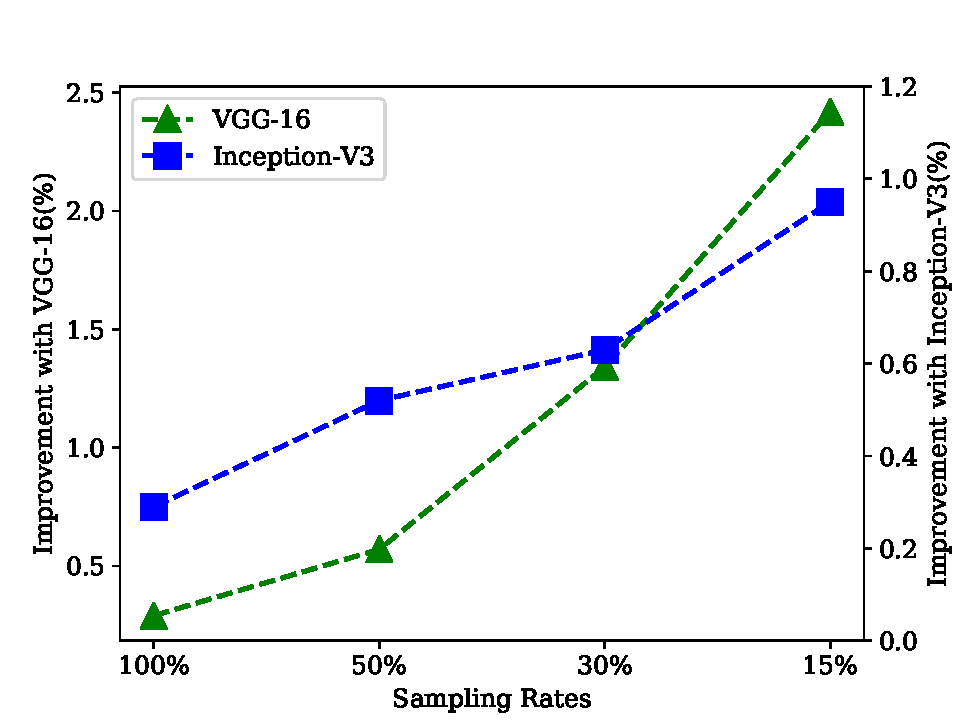
\includegraphics[width=0.48\linewidth]{figures/backbone.pdf}}
  \subcaptionbox{使用不同的初始化方法\label{fig:method}}
    {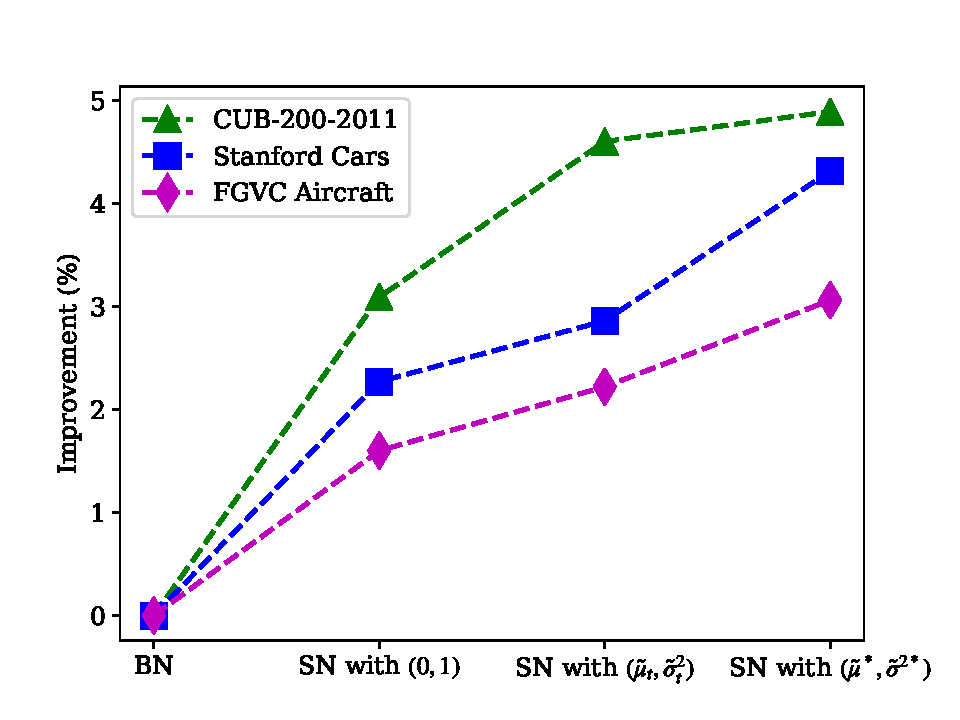
\includegraphics[width=0.48\linewidth]{figures/method.pdf}}
  \subcaptionbox{使用不同的分支选取概率\label{fig:p_acc}}
    {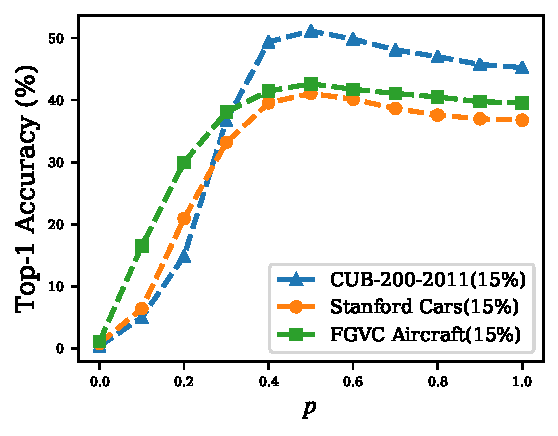
\includegraphics[width=0.48\linewidth]{figures/p_acc.pdf}}
  \caption{分析实验}
\end{figure}

\textbf{不同初始化方法的比较 } 为了更好的理解StochNorm,本文在~\ref{section:settings}中提到的三个细粒度分类数据集进行$15\%$采样,然后对StochNorm的几个变种进行了消融实验(Ablation Study)。StochNorm的主要创新点来自于双分支的设计以及在分支
间进行随机选择。这种设计也意味着,额外加入的使用$\tilde{\mu}, \tilde{\sigma}^2$进行标准化的分支,对网络的训练有很大的影响。由于在模型微调阶段,可以很自然地使用预训练模型中的$\tilde{\mu}^*, \tilde{\sigma}^{2^*}$作为其初始值,
本文在这里对不同的初始化方法进行了比较:
\begin{itemize}
  \item 使用$(\vec{0}, \vec{1})$作为初始值;
  \item 使用$\tilde{\mu}^*, \tilde{\sigma}^{2^*}$作为初始值;
  \item 使用$\tilde{\mu}_t, \tilde{\sigma}_t^2$作为初始值,其中$\tilde{\mu}_t, \tilde{\sigma}_t^2$使用目标域数据在预训练模型上前向反馈计算得到。
\end{itemize}

三个变种方法相对BatchNorm在三个数据集上的平均绝对提升如图~\ref{fig:method}所示。可以看出,$\tilde{\mu}^*, \tilde{\sigma}^{2^*}$的效果最好,而$(\vec{0}, \vec{1})$的效果最差。可以看出,尽管绝对提升没有随机选择的双分支结构高,但使用
包含着更多关于预训练数据以及模型指使的初始值,依然能够在模型微调阶段带来更多提升。

\textbf{不同的分支选取概率 } 作为StochNorm中唯一新增的超参数,分支选取概率$p$的选择对于模型最后的效果提升来说也十分关键,为了进一步分析超参数$p$对StochNorm效果的影响,我们在$15\%$采样的三个细粒度分类数据集上,
对$p$从$0.0$(即完全使用滑动平均估计的统计值进行标准化)到$1.0$(即BatchNorm)间隔$0.1$共$11$个取值分别进行了实验,实验结果如图~\ref{fig:p_acc}所示。可以看出,$p=0.5$在三个数据集上都取得了最好的效果,对于较大
的$p$而言,相对BatchNorm,即$p=0$而言,都有一定的提升,而较小的$p$则会导致网络不收敛,这与许多BatchNorm相关研究工作的结论一致。

% \begin{figure}
%   \centering
%   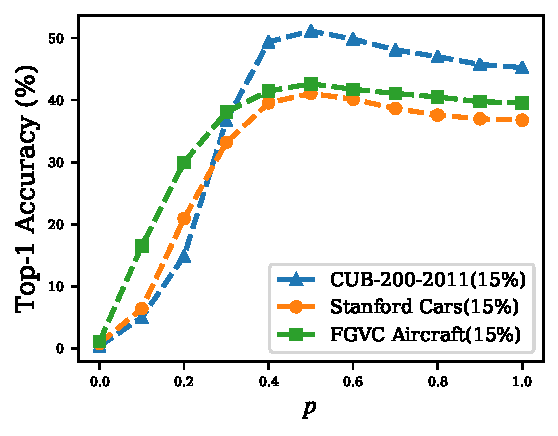
\includegraphics[width=0.5\linewidth]{figures/p_acc.pdf}
%   \caption{StochNorm中超参数$p$的选取对效果的影响}
%   \label{fig:p_acc}
% \end{figure}

\textbf{与模型微调方法相结合 } 本文在这一节的最后,将随机标准化层与前文提到的三种传统的模型微调方法进行结合,进一步展示了该方法的通用性。这里依旧选用节~\ref{section:settings}中三个细粒度分类数据集作为实验场景,预训练
模型依旧选择ResNet-50。实验结果如表\ref{table:combine_cub}、\ref{table:combine_cars}和\ref{table:combine_air}所示,可以很明显地看出,将随机标准化层与其他模型微调方法相结合,在大多数情况下能够进一步提升模型在测试集上的准确率。这是由于随机标准化层是一种网络结果层面
的方法,通过设计更合理地标准化层结构来实现对深度神经网络性能的提升。这与传统的在网络参数、网络特征层面进行正则化约束的模型微调方法是相互正交、相互弥补的。因此,两种方法相结合能够取得更好的效果也是理所当然。


\begin{table*}[htbp]
	\begin{center}
	\caption{与模型微调方法相结合的实验结果 (CUB-200-2011).}
	\label{table:combine_cub}
	\centering
        \begin{tabular}{lcccc} 
            \toprule
            \multirow{2}*{方法} & \multicolumn{4}{c}{数据采样比例} \\
            \cmidrule(lr){2-5}
             & $15\%$ & $30\%$ & $50\%$ & $100\%$ \\
            \midrule
            $L_2$-SP \citep{xuhong2018explicit} & $45.08\pm0.19$ & $57.78\pm0.24$ & $69.47\pm0.29$ & $78.44\pm0.17$ \\
            $L_2$-SP+\textbf{StochNorm} & $49.92\pm0.24$ & $60.48\pm0.12$ & $70.47\pm0.19$ & $79.24\pm0.11$  \\
            \cmidrule(r){1-5}
            DELTA \citep{li2018delta} & $46.83\pm0.21$ & $60.37\pm0.25$ & $71.38\pm0.20$ & $78.63\pm0.18$ \\
            DELTA+\textbf{StochNorm} & $49.27\pm0.31$ & $62.86\pm0.30$ & $72.78\pm0.16$ & $79.72\pm0.12$ \\
            \cmidrule(r){1-5}
            BSS \citep{chen2019catastrophic} & $47.74\pm0.23$ & $62.03\pm0.29$ & $72.56\pm0.17$ & $78.85\pm0.31$  \\ 
            BSS+\textbf{StochNorm} & $50.69\pm0.29$ & $64.10\pm0.18$ & $73.01\pm0.26$ & $79.91\pm0.14$  \\
            \bottomrule
        \end{tabular}
	\end{center}
\end{table*}

\begin{table*}[htbp]
	\begin{center}
	\caption{与模型微调方法相结合的实验结果 (Standford Cars).}
	\label{table:combine_cars}
	\centering
        \begin{tabular}{lcccc} 
            \toprule
            \multirow{2}*{方法} & \multicolumn{4}{c}{数据采样比例} \\
            \cmidrule(lr){2-5}
             & $15\%$ & $30\%$ & $50\%$ & $100\%$ \\
            \midrule
            $L_2$-SP \citep{xuhong2018explicit} & $36.10\pm0.30$ & $60.30\pm0.28$ & $75.48\pm0.22$ & $86.58\pm0.26$ \\
            $L_2$-SP+\textbf{StochNorm} & $40.50\pm0.23$ & $64.86\pm0.32$ & $77.34\pm0.11$ & $86.81\pm0.16$  \\
            \cmidrule(r){1-5}
            DELTA \citep{li2018delta} & $39.37\pm0.34$ & $63.28\pm0.27$ & $76.53\pm0.24$ & $86.32\pm0.20$  \\
            DELTA+\textbf{StochNorm} & $40.77\pm0.19$ & $65.67\pm0.17$ & $77.23\pm0.24$ & $86.51\pm0.15$ \\
            \cmidrule(r){1-5}
            BSS \citep{chen2019catastrophic} & $40.57\pm0.12$ & $64.13\pm0.18$ & $76.78\pm0.21$ & $87.63\pm0.27$  \\
            BSS+\textbf{StochNorm} & $44.04\pm0.21$ & $66.28\pm0.12$ & $78.03\pm0.18$ & $87.85\pm0.25$  \\
            \bottomrule
        \end{tabular}
	\end{center}
\end{table*}

\begin{table*}[htbp]
	\begin{center}
	\caption{与模型微调方法相结合的实验结果 (FGVC Aircraft).}
	\label{table:combine_air}
	\centering
        \begin{tabular}{lcccc} 
            \toprule
            \multirow{2}*{方法} & \multicolumn{4}{c}{数据采样比例} \\
            \cmidrule(lr){2-5}
             & $15\%$ & $30\%$ & $50\%$ & $100\%$ \\
            \midrule
            $L_2$-SP \citep{xuhong2018explicit} & $39.27\pm0.24$ & $57.12\pm0.27$ & $67.46\pm0.26$ & $80.98\pm0.29$ \\
            $L_2$-SP+\textbf{StochNorm} & $42.57\pm0.19$ & $60.16\pm0.28$ & $69.16\pm0.09$ & $81.12\pm0.16$  \\
            \cmidrule(r){1-5}
            DELTA \citep{li2018delta} & $42.16\pm0.21$ & $58.60\pm0.29$ & $68.51\pm0.25$ & $80.44\pm0.20$  \\
            DELTA+\textbf{StochNorm} & $44.10\pm.18$ & $60.13\pm0.22$ & $70.12\pm0.14$ & $81.03\pm0.15$ \\
            \cmidrule(r){1-5}
            BSS \citep{chen2019catastrophic} & $40.41\pm0.12$ & $59.23\pm0.31$ & $69.19\pm0.13$ & $81.48\pm0.18$  \\
            BSS+\textbf{StochNorm} & $43.89\pm0.30$ & $60.25\pm0.19$ & $69.41\pm0.26$ & $81.50\pm0.21$  \\
            \bottomrule
        \end{tabular}
	\end{center}
\end{table*}

\section{本章小结}

本章先介绍了广泛使用的BatchNorm的算法流程以及原理,之后介绍了一系列基于正则化约束的模型微调方法。之后本章在少量样本模型微调的场景下基于BatchNorm的不足与缺陷,设计了新的标准化层结构StochNorm,
并在三个细粒度分类数据集上进行了实验,证明了StochNorm的效果。接下来为了更全面地理解StochNorm,从不同的深度神经网络结构、不同的初始化方式、不同的超参数选取以及与不同的模型微调方法相结合四个角度
进行了分析性实验,进一步证明了StochNorm的有效性和通用性。
% !TeX root = ../thuthesis-example.tex

\chapter{实际场景中的应用}

本节主要介绍随机标准化层在两个实际场景——医疗影像诊断和风速预测中的应用情况,以及算法库集成的相关工作。

\section{医疗影像诊断}

\subsection{应用背景}

2020年至今,新冠肺炎在世界范围内流行开来,对全人类的生命健康安全带来了巨大的威胁。在这场疫情中,各行各业都为抗击疫情做出了贡献,而计算机视觉技术则在新冠肺炎的辅助诊断领域有着
不错的效果。对于很多疾病,首先需要通过X光透射、CT扫描或者核磁共振等手段对有疑似病灶的部位进行检查,有经验的医生能通过检查得到的图像进行快速诊断。但是当疫情快速蔓延时,相关专业人士
的数量往往不足以支撑大量的疾病诊断,这时便可以借助计算机视觉技术进行辅助诊断。

\begin{figure}
  \centering
  \subcaptionbox{Infiltration, Nodule and Mass}
    {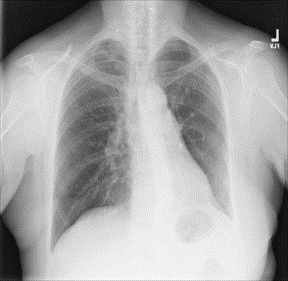
\includegraphics[width=0.3\linewidth]{figures/nih/1.png}}
  \subcaptionbox{Effusion, Infiltration, Nodule and Consolidation}
    {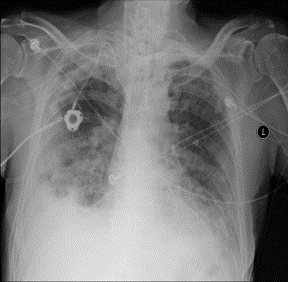
\includegraphics[width=0.3\linewidth]{figures/nih/2.png}}
  \subcaptionbox{Effusion, Infiltration, Atelectasis and Edema}
    {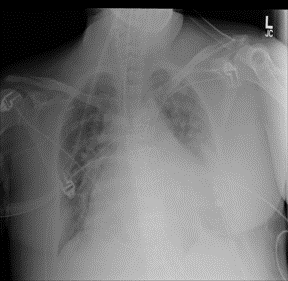
\includegraphics[width=0.3\linewidth]{figures/nih/3.png}}
  \caption{NIH Chest X-ray数据集示例}
  \label{fig:nih}
\end{figure}

医疗影像数据相比传统的图像数据来说,最大的特点便是数据的采集非常耗时耗力,同时数据的标注也非常困难,导致有标注的数据更加稀缺,如何利用稀少但是珍贵的有标注数据来提高模型的诊断准确率,是
计算机视觉技术在医疗影像数据领域的一大难题。除此之外,医疗影像数据还有采集方式与常见的RGB图像有一定区别、病患相关的数据需要脱敏处理、不同疾病的拍摄部位区别很大等诸多问题。因此医疗影像诊断这一
任务,是检验计算机视觉相关算法落地能力的一个重要场景。

\subsection{实验设计}

本节选用了两个基于肺部X光和CT影像的医疗数据集——NIH Chest X-ray~\citep{wang2017chestxray}和COVID-CT~\citep{he2020sample}进行实验。NIH Chest X-ray包含了来自约$3$万名患者
超过$11$万张的肺部正面X光影像,共有$14$种肺部疾病类别(每一张图像可能属于多个类别),是一个多标签的图像分类任务;COVID-CT则包含了来自$216$名新冠肺炎患者的$349$张CT影像,以及大量
正常人的CT影响作为对照,是一个图像二分类任务。图~\ref{fig:nih}和图~\ref{fig:covid}分别展示了两个数据集内的一些图片示例。可以看出,医疗影像相比传统的图像数据来说细节更多,更难以区分,
进行诊断需要极强的专业知识,因此也给了深度学习相关技术开阔的发挥空间。


\begin{figure}
  \centering
  \subcaptionbox{阴性}{
    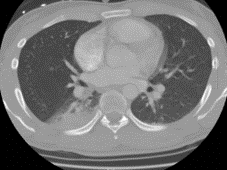
\includegraphics[width=0.45\linewidth]{figures/covid-ct/1.png}
    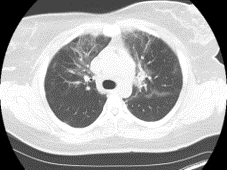
\includegraphics[width=0.45\linewidth]{figures/covid-ct/2.png}
  }
  \subcaptionbox{阳性}{
    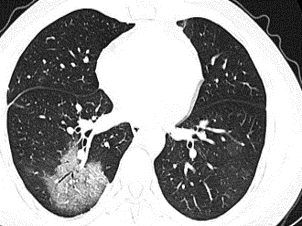
\includegraphics[width=0.45\linewidth]{figures/covid-ct/3.png}
    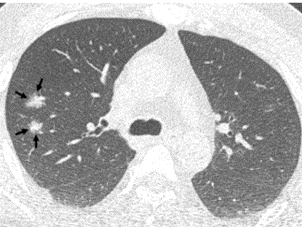
\includegraphics[width=0.45\linewidth]{figures/covid-ct/4.png}
  }
  \caption{COVID-CT数据集示例}
  \label{fig:covid}
\end{figure}


NIH Chest X-ray数据集的数据来自于很多个国家和地区,因此包含着上万条数据用于训练,但是在实际场景中医疗数据的采集耗时耗力,还要考虑信息脱敏等额外隐患,所以很难拥有如此多的数据。所以在本文的实验中,
我们对NIH Chest X-ray数据集进行了三个比例的数据采样——$5\%$、$10\%$和$15\%$,以验证在更符合实际场景的情况下,StochNorm以及一系列主流的模型微调方法能否取得更好的效果。由于数据可能包含多个标签,
作为一个多标签的分类任务,本文使用在14种疾病的的平均AUC作为验证指标,预训练模型选择ResNet-50。

相比起NIH Chest X-ray数据集而言,COVID-CT数据集则更贴近现实场景下的医疗数据集、由于新冠肺炎是近年来新出现的疾病,所以数据集中只包含了几百张新冠肺炎的正样本CT影像,能够更好地验证模型微调方法在实际场景中
是否有作用,是否能够更大程度地利用预训练模型的知识,在稀少却很珍贵的数据上训练得到更好的效果。本文依然比较了StochNorm以及一系列主流的模型微调方法,验证指标选择AUC,预训练模型选择ResNet-50。

\subsection{实验结果} 

两个数据集上的实验结果如表~\ref{table:chexray}和表~\ref{table:covid-ct}所示。Raghu\citep{raghu2019transfusion}等人的工作发现,由于广泛使用的预训练模型使用的数据和实际场景中的医疗数据之间有着巨大的领域差异,
因而在这些医疗数据集上,传统的$L_2$模型微调无法取得足够明显的提升。本文的实验也证实了,很多在常规数据集上表现较好的基于正则化约束项的模型微调方法,在医疗数据集上反而会带来负收益。但是相反的,作为一种结构化的隐式正则方法,
通过简单地将BatchNorm替换为StochNorm,能够在COVID-CT数据集上有$\textbf{3.13\%}$的AUC提升,在NIH Chest X-ray数据集的三个采样比例下也取得了平均$\textbf{1.1\%}$的AUC提升。这说明了,在数据量不够充足的情况下,模型微调的方法依然有很多提升的空间。

\begin{table*}[h]
	\begin{center}
  \caption{NIH Chest X-ray数据集实验结果}
	\label{table:chexray}
    \begin{tabular}{lccc}
        \toprule
        \multirow{2}*{方法} & \multicolumn{3}{c}{数据采样比例} \\
        \cmidrule(r){2-4}
          & $5\%$ & $10\%$ & $15\%$ \\
        \midrule
        Baseline($L_2$) & $70.37\pm0.31$ & $75.85\pm0.22$ & $76.64\pm0.11$ \\
        $L_2$-SP \citep{xuhong2018explicit} & $70.02\pm0.27$ & $72.73\pm0.41$ & $75.71\pm0.22$  \\
        DELTA \citep{li2018delta} & $70.99\pm0.19$ & $74.35\pm0.20$ & $75.97\pm0.17$ \\
        BSS \citep{chen2019catastrophic} & $69.86\pm0.12$ & $73.27\pm0.19$ & $76.10\pm0.23$  \\
        \cmidrule(r){1-4}
        \textbf{StochNorm} & $\textbf{72.50}\pm\textbf{0.26}$ & $\textbf{76.48}\pm\textbf{0.15}$ & $\textbf{77.01}\pm\textbf{0.21}$ \\
        \bottomrule
    \end{tabular}
	\end{center}
\end{table*}


\begin{table*}[h]
	\begin{center}
  \caption{COVID-CT数据集实验结果}
	\label{table:covid-ct}
    \begin{tabular}{lccccccccc}
        \toprule
        Baseline($L_2$) & $L_2$-SP \citep{xuhong2018explicit} & DELTA \citep{li2018delta} & BSS \citep{chen2019catastrophic} &  \textbf{StochNorm}\\
        \midrule
        $87.30\pm0.20$ & $85.11\pm0.13$ & $87.79\pm0.24$ & $88.52\pm0.31$ & $90.43\pm0.15$\\
        \bottomrule
    \end{tabular}
	\end{center}
\end{table*}

\section{金风风速预测}

\subsection{应用背景}

2020年9月我国明确提出“双碳”战略,即2030年“碳达峰”与2060年“碳中和”目标。对于燃烧煤炭进行火力发电这种传统的发电方式,碳排放量极大,与“双碳”战略相斥,需要被逐步取代,而诸如利用风能等
清洁能源进行发电的方式逐渐受到重视。我们国家地大物博,风能资源丰富,在许多地方都有面积巨大的风场,如何利用这些风场高效发电,是当下的热点问题。对于传统火力发电而言,发电功率取决于
煤炭燃烧的速率,能够被人为地控制,而风力发电的功率则主要取决于风速,具有很强的随机性和不可控性。因此,如果能较为准确地预测未来的风速变化趋势,对于电厂进行统筹规划来说又很大的意义。

\begin{figure}
  \centering
  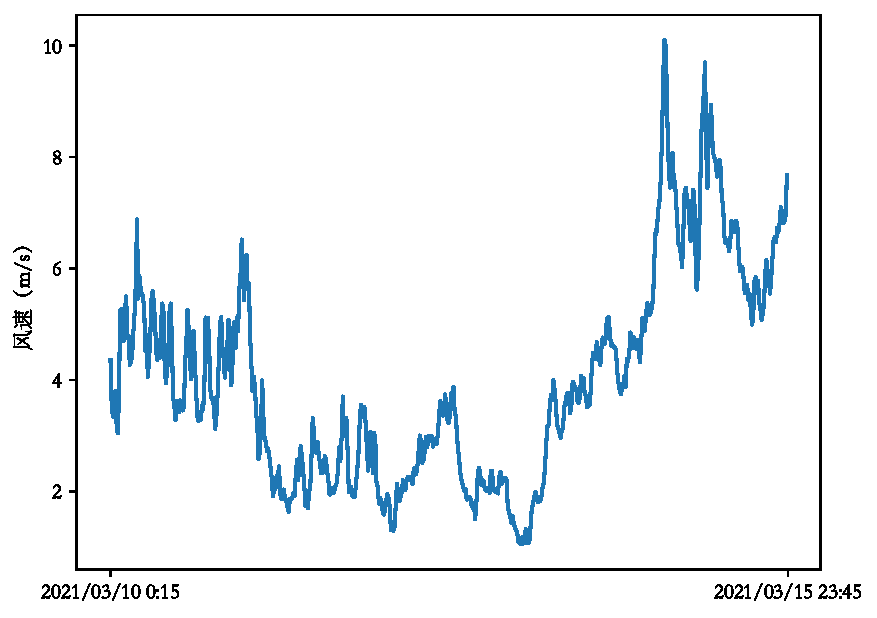
\includegraphics[width=0.75\linewidth]{figures/wind.pdf}
  \caption{金风风速数据示例}
  \label{fig:goldwind}
\end{figure}

在不同地区、不同季节、不同时间风场的风速都有所不同,而风场的各种气象特征都与风速的变化息息相关。当下的前沿工作主要采用数值天气预报来预测风速,数值天气预报可以通过卫星、雷达、气象站等方式获取,
包括不同高度的温度、湿度、压强、云量等气象指标,为接下来进行风速预测提供了数据基础。风速预测一般按照预测时长分为三类:短期、中期和长期风速预测,预测的时间区间从几天到几个月甚至一年以上,相应的
预测精度要求也会随时间增加而降低。

本文涉及的项目为金风风速预测项目,主要的目标为进行短期的风速预测,即预测$3km\times3km$空间内在未来$8$天左右的风速情况,时间间隔为$15$分钟,属于精度要求较高的一种风速预测任务。图~\ref{fig:goldwind}
为2021年3月的风速观测曲线。对于该任务而言,主要面临的困难在于金风风场的风速数据变化大、抖动多、噪声多等问题,气象预报数据种类非常多,并且存在不可避免的误差,很容易在训练数据上出现过拟合的现象,缺乏泛化性和
迁移性。同时,由于数据中同时包含气象预报数据和风速数据,与学术界时间序列研究的问题设定有很多不同,需要针对实际场景进行设计与调整,为深度学习算法的实际落地带来了很多阻碍。

\begin{figure}
  \centering
  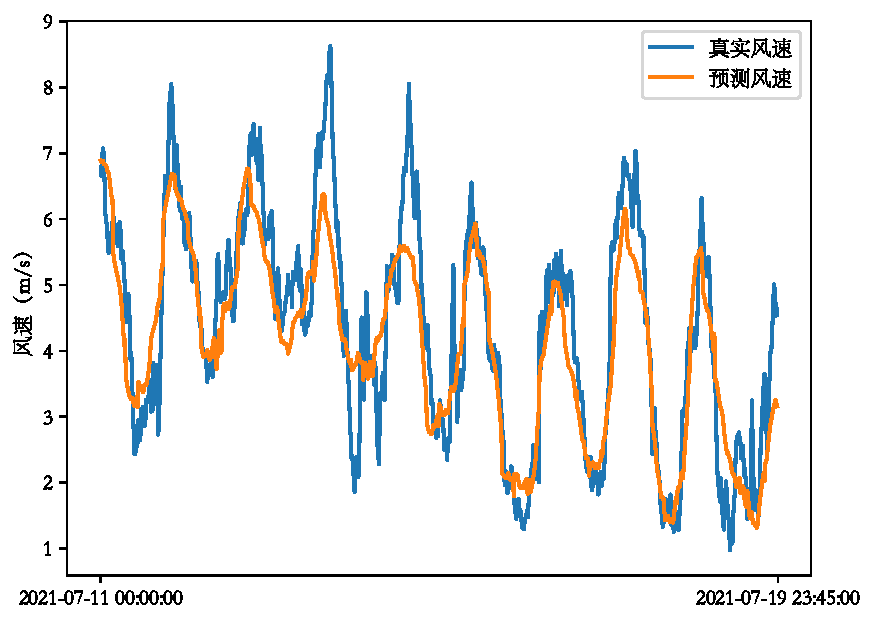
\includegraphics[width=0.75\linewidth]{figures/wind2.pdf}
  \caption{金风风速真实曲线与预测曲线}
  \label{fig:pred}
\end{figure}

\begin{table*}[h]
	\begin{center}
  \caption{金风风速预测数据集实验结果}
	\label{table:goldwind}
    \begin{tabular}{ccccc}
        \toprule
        训练数据 & 测试数据 & 金风基线指标 & Baseline &  Baseline+\textbf{StochNorm}\\
        \midrule
        03/01-05/30 & 05/31-06/10 & 1.433 & 1.337 & 1.264 \\
        03/11-06/10 & 06/11-06/20 & 1.183 & 0.777 & 0.789 \\
        03/21-06/20 & 06/21-06/30 & 1.090 & 1.225 & 1.181 \\
        \cmidrule(r){1-5}
        04/01-06/30 & 07/01-07/10 & 1.093 & 0.946 & 1.066 \\
        04/11-07/10 & 07/11-07/20 & 1.159 & 0.830 & 0.794 \\
        04/21-07/20 & 07/21-07/30 & 1.184 & 1.511 & 1.474 \\
        \cmidrule(r){1-5}
        05/01-07/30 & 07/31-08/10 & 1.302 & 1.393 & 1.271 \\
        05/11-08/10 & 08/11-08/20 & 1.014 & 1.055 & 0.908 \\
        05/21-08/20 & 08/21-08/30 & 1.084 & 1.030 & 0.874 \\
        \cmidrule(r){1-5}
        06/01-08/30 & 08/31-09/10 & 1.038 & 0.880 & 0.859 \\
        06/11-09/10 & 09/11-09/20 & 1.262 & 1.200 & 1.339 \\
        06/21-09/20 & 09/21-09/30 & 1.201 & 1.081 & 1.071 \\
        \midrule
        \multicolumn{2}{c}{平均值} & 1.170 & 1.105 & 1.074 \\
        \bottomrule
    \end{tabular}
	\end{center}
\end{table*}

\subsection{实验设计}

本节选择了金风风速预测数据集中的广西风场数据作为实验数据集。数据集包含了2021年3月至9月共计7个月内的气象数据预报数据,比如压强、温度、湿度等气象数据,以及每个时间点测量点测
量得到的风速。本文选择连续3个月的气象数据以及风速作为深度神经网络的训练输入,之后以接下来10天的气象预报数据作为测试输入,来预测接下来10天每个时间节点的实时风速,属于包含
时序数据的回归问题。训练数据在3到9月的时间节点上,以三个月为训练区间,10天为间隔做平移,共得到12组训练-测试数据对。深度神经网络结构方面使用三层MLP作为回归器,通过某一时刻的气象预报
数据来回归预测相应的风速,同时加入Transformer利用预测的历史风速和真实的历史风速数据,捕捉风速之间的时序关系,从而基于未来的气象预报数据预测风速。为了验证StochNorm在该场景下的效果,
本文将原网络结构中的标准化层替换为StochNorm,验证指标为10天内风速预测的均方根误差(Root Mean Squared Error, RMSE)。

\subsection{实验结果}

实验结果如表~\ref{table:goldwind}所示,可以看出MLP+Transformer的网络结构相比金风提供的基线指标有一定的提升,而在更换为StochNorm之后,模型的RMSE有了进一步的下降,12组数据上相比基线
指标的相对提升平均为$\textbf{8.21\%}$。通过进一步的分析发现,由于风速与同一时刻的很多气象特征有着强相关性,使得在某一时间训练的模型很容易出现过拟合的现象,而由于不同时刻的风速随机性较强,
过拟合的模型在训练时间段以外的效果可能会变差。图~\ref{fig:pred}展示了预测的风速曲线与实际风速曲线的比较。StochNorm作为一种在模型微调场景下提出的标准化层,就具有着在模型训练阶段一定程度上避免过拟合的效果,因此直接应用在风速预测的场景中,能进一步提高
模型的泛化性,提升验证指标。




\section{迁移学习算法库集成}

\subsection{迁移学习算法库介绍}

迁移学习算法库(Transfer-Learning-Library)是清华大学大数据软件团队机器学习组推出的一个专门面向迁移学习算法的算法库,针对迁移学习中的多个分支问题,例如领域适应学习(Domain Adaptation)、
模型微调(Model Fine-tune)、领域泛化学习(Domain Generalization)等,整理组内提出的以及学术界经典以及前沿的相关深度学习算法,使用统一的代码框架、统一的数据集以及训练-验证流程进行实验,从而
在不同算法间进行相对公平的比较。该算法库基于PyTorch实现,为整个机器学习组的工作,本文仅提供了StochNorm相关的算法实现与集成。

\subsection{集成效果}

本文基于迁移学习算法库针对模型微调任务的的通用框架,对StochNorm的算法进行了实现与集成,集成效果如表~\ref{table:cub_2}、\ref{table:cars_2}和\ref{table:air_2}所示。算法库在本文涉及的三个细粒
度分类数据集上进行了实验,由于数据划分以及验证方式的不同,所有方法的最终效果相比节\ref{section:results}中均有一定提升。但是在迁移学习算法库这一相对公平的比较平台上,StochNorm相较于基线指标依然
取得了较为明显的提升,尤其在数据量较少的任务中($15\%$和$30\%$的数据采样比例)。通过在迁移学习算法库中进行集成,StochNorm能够通过算法库的API进行快速调用,有助于在各种学术研究和实际任务中得到应用,进一步推动深度学习领域的不断发展。


\begin{table*}[h]
	\begin{center}
	\caption{实验结果(CUB-200-2011)}
	\label{table:cub_2}
	\centering
    \resizebox{\textwidth}{!}{
      \begin{tabular}{lccccccc}
          \toprule
          \multirow{2}*{数据采样比例} & \multicolumn{7}{c}{方法} \\
          \cmidrule(r){2-8}
          & Baseline($L_2$) & LWF \citep{li2017learning} & BSS \citep{chen2019catastrophic} & DELTA \citep{li2018delta} & \textbf{StochNorm} & Co-Tuning \citep{you2020co} & Bi-Tuning \citep{zhong2020bi} \\
          \midrule
          $15\%$ & $51.2$ & $56.7$ & $53.4$ & $54.8$ & $54.8$ & $57.6$ & $55.8$ \\
          $30\%$ & $64.6$ & $66.8$ & $66.7$ & $67.3$ & $66.8$ & $70.1$ & $69.3$ \\
          $50\%$ & $74.6$ & $73.4$ & $76.0$ & $76.3$ & $75.8$ & $77.3$ & $77.2$ \\ 
          $100\%$ & $81.8$ & $81.5$ & $82.0$ & $82.3$ & $82.2$ & $82.5$ & $83.1$ \\
          \cmidrule(r){1-8}
          平均值 & $68.1$ & $69.6$ & $69.5$ & $70.2$ & $69.9$ & $71.9$ & $71.4$ \\
          \bottomrule
      \end{tabular}
    }
	\end{center}
\end{table*}

\begin{table*}[h]
	\begin{center}
	\caption{实验结果(Standford Cars)}
	\label{table:cars_2}
	\centering
    \resizebox{\textwidth}{!}{
      \begin{tabular}{lccccccc}
          \toprule
          \multirow{2}*{数据采样比例} & \multicolumn{7}{c}{方法} \\
          \cmidrule(r){2-8}
          & Baseline($L_2$) & LWF \citep{li2017learning} & BSS \citep{chen2019catastrophic} & DELTA \citep{li2018delta} & \textbf{StochNorm} & Co-Tuning \citep{you2020co} & Bi-Tuning \citep{zhong2020bi} \\
          \midrule
          $15\%$ & $41.1$ & $44.9$ & $43.3$ & $45.0$ & $44.4$ & $49.0$ & $48.3$ \\
          $30\%$ & $65.9$ & $67.0$ & $67.6$ & $68.4$ & $68.1$ & $70.6$ & $72.8$ \\
          $50\%$ & $78.4$ & $77.6$ & $79.6$ & $79.6$ & $79.3$ & $81.9$ & $83.3$ \\ 
          $100\%$ & $87.8$ & $87.5$ & $88.0$ & $88.4$ & $87.9$ & $89.1$ & $90.2$ \\
          \cmidrule(r){1-8}
          平均值 & $68.3$ & $69.3$ & $69.6$ & $70.4$ & $69.9$ & $72.7$ & $73.7$ \\
          \bottomrule
      \end{tabular}
    }
	\end{center}
\end{table*}

\begin{table*}[h]
	\begin{center}
	\caption{实验结果(FGVC Aircraft)}
	\label{table:air_2}
	\centering
    \resizebox{\textwidth}{!}{
      \begin{tabular}{lccccccc}
          \toprule
          \multirow{2}*{数据采样比例} & \multicolumn{7}{c}{方法} \\
          \cmidrule(r){2-8}
          & Baseline($L_2$) & LWF \citep{li2017learning} & BSS \citep{chen2019catastrophic} & DELTA \citep{li2018delta} & \textbf{StochNorm} & Co-Tuning \citep{you2020co} & Bi-Tuning \citep{zhong2020bi} \\
          \midrule
          $15\%$ & $41.6$ & $44.1$ & $43.6$ & $44.4$ & $44.3$ & $45.9$ & $47.2$ \\
          $30\%$ & $57.8$ & $60.6$ & $59.5$ & $61.9$ & $60.6$ & $61.2$ & $64.3$ \\
          $50\%$ & $68.7$ & $68.7$ & $69.6$ & $71.4$ & $70.1$ & $71.3$ & $73.7$ \\ 
          $100\%$ & $80.2$ & $82.4$ & $81.2$ & $82.7$ & $81.5$ & $82.2$ & $84.3$ \\
          \cmidrule(r){1-8}
          平均值 & $62.1$ & $64.0$ & $63.5$ & $65.1$ & $64.1$ & $65.2$ & $67.4$ \\
          \bottomrule
      \end{tabular}
    }
	\end{center}
\end{table*}

\section{本章小结}

本章展示了本文提出的标准化层结构StochNorm在医疗影像诊断、风速预测等实际场景中的具体应用,以及在迁移学习算法库中的集成效果。
% !TeX root = ../thuthesis-example.tex

\chapter{总结与展望}

\section{本文工作总结}

本文主要研究了在模型微调场景下批标准化BatchNorm存在的缺陷与不足,并基于双分支结构和随机前向传播的思想,针对模型微调场景设计了新的标准化层结构,随机标准化层StochNorm。

本文在三个细粒度分类数据集上验证了StochNorm的性能,证明了在数据量较少的模型微调场景下,StochNorm具有超过主流的基于正则化约束的模型微调方法的性能。同时本文还将StochNorm与多种不同的深度
神经网络结构以及模型微调方法进行了结合,进一步取得了效果上的提升,从而也展示了StochNorm作为一种网络结构层面方法的通用性。

本文还展示了StochNorm在两个实际场景,医疗影像诊断和风速预测中的应用。通过在现有模型中加入StochNorm技术,能够获得一定的效果提升。最后本文还基于迁移学习算法库的平台,对StochNorm进行了算法
集成,提供了方便快捷调用的API接口。

\section{未来工作展望}

\textbf{标准化技术的发展 } 本文在提出StochNorm的同时,也对目前广泛使用的BatchNorm中存在的问题进行了一定的分析。尽管类似BatchNorm的常用的标准化层结构已经在各领域的各类任务中取得了喜人的成果,
其中存在的很多不足与缺陷也不能忽略。同时,许多标准化技术的作用原理仍然没有得到解释,实验性的结果也需要扎实的理论分析来肯定。相信今后也会有越来越多的研究人员开始对这些经典的方法进行
深入的分析与改进,提出更泛用更有效的标准化技术。

\textbf{随机性在深度学习中的应用 } 本文提出的StochNorm的一大创新点便是将随机性引入了标准化层结构,实现了一种隐式的结构层面正则化约束。随机性对于深度学习而言有着非常重要的意义,从神经
元随机失活(Dropout)到输入数据的随机增广(Augmentation),随机性的引入为深度学习带来了更大的可能性。如今很多新的研究工作也通过掩码技术、对比学习等方式将随机性从不同的角度引入深度学习
当中,相信未来也能看到更多随机性在深度学习中的应用。

\textbf{挖掘预训练模型的潜力 } 
目前模型微调领域的工作往往都会人为地区分为预训练阶段和微调阶段。但是预训练与微调本应是有机的整体,人为地进行区分就会经常出现预训练模型与下游任务差异过大,带来负收益的现象。如今有越来越多的研究人员
开始重视这一观点,诸如针对微调任务的特征利用元学习(Meta Learning)的技术设计预训练模型,获得对下游任务更有意义的预训练模型。

同时,预训练模型中包含的知识也并非只有可学习的网络参数。本文提出的StochNorm中,通过双分支的结构,巧妙地将预训练模型中以往被忽视的统计类参数引入了模型微调阶段,进一步挖掘了预训练模型
中的知识。如今也有很多新的工作开始重视预训练模型中可学习的网络参数之外的信息,包括深度神经网络优化器、预训练使用的数据增广甚至预训练阶段的的梯度信息等,从更多的维度对预训练模型进行分析,
相信未来能看到对预训练模型中潜力的充分挖掘。


\textbf{更多的应用场景 } 除了本文提到的两个应用场景外,深度学习还有很广泛的应用场景,诸如目标检测、实例分割、关键点检测等多种任务。在这些任务中,也依然存在着数据量不足的问题,如何更好地
利用现有的知识来提升训练效果,以及如何避免数据量不足带来的问题,都是值得进一步研究的问题。相信今后的研究工作一定能在这些领域获得突破。



% 其他部分
\backmatter

% 参考文献
\bibliography{ref/refs}  % 参考文献使用 BibTeX 编译
% \printbibliography       % 参考文献使用 BibLaTeX 编译

% 附录
% 本科生需要将附录放到声明之后,个人简历之前
\appendix
% \input{data/appendix-survey}       % 本科生:外文资料的调研阅读报告
% \input{data/appendix-translation}  % 本科生:外文资料的书面翻译
\input{data/appendix}

% 致谢
\input{data/acknowledgements}

% 声明
\statement
% 将签字扫描后的声明文件 scan-statement.pdf 替换原始页面
% \statement[file=scan-statement.pdf]
% 本科生编译生成的声明页默认不加页脚,插入扫描版时再补上;
% 研究生编译生成时有页眉页脚,插入扫描版时不再重复。
% 也可以手动控制是否加页眉页脚
% \statement[page-style=empty]
% \statement[file=scan-statement.pdf, page-style=plain]

% 个人简历、在学期间完成的相关学术成果
% 本科生可以附个人简历,也可以不附个人简历
% !TeX root = ../thuthesis-example.tex

\begin{resume}

  \section*{个人简历}

  1997 年 8 月 28 日出生于山西省忻州市。

  2015 年 9 月考入清华大学环境学院环境工程专业,2016 年 9 月转入软件学院软件工程专业,2019 年 7 月本科毕业并获得理学学士学位。

  2019 年 9 月免试进入清华大学软件学院攻读软件工程专业工学硕士至今。


  \section*{在学期间完成的相关学术成果}

  \subsection*{学术论文}

  \begin{achievements}
    \item Kou Z, You K, Long M, et al. Stochastic normalization[J]. Advances in Neural Information Processing Systems, 2020, 33: 16304-16314.
    \item You K, Kou Z, Long M, et al. Co-tuning for transfer learning[J]. Advances in Neural Information Processing Systems, 2020, 33: 17236-17246.
    \item Shu Y, Kou Z, Cao Z, et al. Zoo-tuning: Adaptive transfer from a zoo of models[C]//International Conference on Machine Learning. PMLR, 2021: 9626-9637.
    \item Zhong J, Wang X, Kou Z, et al. Bi-tuning of pre-trained representations[J]. arXiv preprint arXiv:2011.06182, 2020.
  \end{achievements}

\end{resume}


% 指导教师/指导小组学术评语
% 本科生不需要
\input{data/comments}

% 答辩委员会决议书
% 本科生不需要
\input{data/resolution}

% 本科生的综合论文训练记录表(扫描版)
% \record{file=scan-record.pdf}

\end{document}
